% arara: pdflatex: { synctex: yes }
% arara: makeindex: { style: ctuthesis }
% arara: bibtex

% The class takes all the key=value arguments that \ctusetup does,
% and a couple more: draft and oneside
\documentclass[twoside]{ctuthesis}

\usepackage[utf8]{inputenc}
\usepackage{caption}
\usepackage{subcaption}
\usepackage{tikz}
\usetikzlibrary{shapes.geometric}
\usetikzlibrary{arrows.meta,arrows}
\usepackage[demo,abs]{overpic}
% Pictures
\usepackage{graphicx,import}
\graphicspath{ {images/svg/} {images/svg/otopna-soustava/} {images/svg/software/}}
% Table
\usepackage{multirow}
\usepackage{slashbox}

\usepackage{makecell}
\renewcommand\theadfont{\bfseries}


% Notes
\usepackage{threeparttable}

% List of terms and abbreviations
\usepackage[automake,acronym,nonumberlist]{glossaries}

% Bibtex
% Zalomeni dlouheho url
\usepackage{xurl}

% Zamezeni parchantum
\usepackage{nowidow}

% Vlozeni PDF souboru
\usepackage{pdfpages}

% Balicek na posunuti cislovani stranek u PDF prilohy
\usepackage{fancyhdr}
% Importovani text souboru z podslozek
\usepackage{import}

% Rotace obrázku pro blokové schéma HA
\usepackage{rotating}
%\usepackage{tikz}



\ctusetup{
	%preprint = \ctuverlog,
%	mainlanguage = english,
	titlelanguage = czech,
	mainlanguage = czech,
	otherlanguages = {slovak,english},
	title-czech = {Systém pro podlahové vytápění rodinného domu pomocí zónové regulace},
	title-english = {System for underfloor heating of a family house using zone control},
%	subtitle-czech = {Cesta do tajů kdovíčeho},
%	subtitle-english = {Journey to the who-knows-what wondeland},
	doctype = M,
	faculty = F3,
	department-czech = {Katedra mikroelektroniky},
	department-english = {Department of Microelectronics},
	author = {Bc. Roman Labovský},
	supervisor = {Ing. Vladimír Janíček, Ph.D.},
	supervisor-address = {České vysoké učení technické v Praze, Fakulta elektrotechnická, Katedra mikroelektroniky\\ Technická 2, \\ Praha 6 \\ 166 27},
%	supervisor-specialist = {John Doe},
	fieldofstudy-english = {Electronics},
	subfieldofstudy-english = {Electronics and Communication},
	fieldofstudy-czech = {Elektronika},
	subfieldofstudy-czech = {Elektronika a komunikace},
	keywords-czech = {termostat, Home Assistant, zónová regulace vytápění, podlahové vytápění, Power over Ethernet, ESP32 },
	keywords-english = {thermostat, Home Assistant, zone heating control, floor heating, Power over Ethernet, ESP32},
	day = 1,
	month = 1,
	year = 2022,
	specification-file = {zadani-dp.pdf},
	front-specification = true,
%	front-list-of-figures = false,
%	front-list-of-tables = false,
%	monochrome = true,
%	layout-short = true,
	pkg-listings = true,
}

\ctuprocess

\addto\ctucaptionsczech{%
	\def\supervisorname{Vedoucí}%
	\def\subfieldofstudyname{Studijní program}%
}

\ctutemplateset{maketitle twocolumn default}{
	\begin{twocolumnfrontmatterpage}	
		\ctutemplate{twocolumn.thanks}
		\ctutemplate{twocolumn.declaration}
		\ctutemplate{twocolumn.abstract.in.titlelanguage}
		\ctutemplate{twocolumn.abstract.in.secondlanguage}
		\ctutemplate{twocolumn.tableofcontents}
		\ctutemplate{twocolumn.listoffigures}
	\end{twocolumnfrontmatterpage}
}

% Posunuti cislovani stranky dolu u vlozenych PDF (priloha)
\fancypagestyle{includedpages}{%
  \fancyhf{}%
  \renewcommand{\headrulewidth}{0pt}%
  \setlength{\footskip}{70pt}
  \fancyfoot[C]{\thepage}%
}

% Seznam prilohy
\newcommand\listappendixname{Seznam příloh}
\newcommand\appcaption[1]{%
   \addcontentsline{app}{chapter}{#1}}
\makeatletter
\newcommand\listofappendices{%
   \section*{\listappendixname}\@starttoc{app}}

% Diakritika pro listings (zapis kodu)
\lstset{
     literate=%
         {á}{{\'a}}1
         {í}{{\'i}}1
         {é}{{\'e}}1
         {ý}{{\'y}}1
         {ú}{{\'u}}1
         {ó}{{\'o}}1
         {ě}{{\v{e}}}1
         {š}{{\v{s}}}1
         {č}{{\v{c}}}1
         {ř}{{\v{r}}}1
         {ž}{{\v{z}}}1
         {ď}{{\v{d}}}1
         {ť}{{\v{t}}}1
         {ň}{{\v{n}}}1                
         {ů}{{\r{u}}}1
         {Á}{{\'A}}1
         {Í}{{\'I}}1
         {É}{{\'E}}1
         {Ý}{{\'Y}}1
         {Ú}{{\'U}}1
         {Ó}{{\'O}}1
         {Ě}{{\v{E}}}1
         {Š}{{\v{S}}}1
         {Č}{{\v{C}}}1
         {Ř}{{\v{R}}}1
         {Ž}{{\v{Z}}}1
         {Ď}{{\v{D}}}1
         {Ť}{{\v{T}}}1
         {Ň}{{\v{N}}}1                
         {Ů}{{\r{U}}}1    
}

% Theorem declarations, this is the reasonable default, anybody can do what they wish.
% If you prefer theorems in italics rather than slanted, use \theoremstyle{plainit}
\theoremstyle{plain}
\newtheorem{theorem}{Theorem}[chapter]
\newtheorem{corollary}[theorem]{Corollary}
\newtheorem{lemma}[theorem]{Lemma}
\newtheorem{proposition}[theorem]{Proposition}

\theoremstyle{definition}
\newtheorem{definition}[theorem]{Definition}
%\newtheorem{example}[theorem]{Example}
\newtheorem{conjecture}[theorem]{Conjecture}

\theoremstyle{note}
\newtheorem*{remark*}{Remark}
\newtheorem{remark}[theorem]{Remark}
% Velikost mezery mezi odstavci
\setlength{\parskip}{2.5ex plus 0.2ex minus 0.2ex}

% Abstract in Czech
\begin{abstract-czech}
Tato diplomová práce se zabývá problematikou regulace zónového podlahového vytápění domácnosti. Pro řízení se využívá systém Home Assistant fungující na Raspberry Pi, který je ovladatelný přes webové rozhraní. V rámci systému jsou vybraná nebo zhotovená zařízení pro ovládání jednotlivých částí zónové regulace vytápění a lokální snímače prostorové teploty. Následně je celý řídicí systém testován a používán v reálném prostředí.
\end{abstract-czech}

% Abstract in English
\begin{abstract-english}
This thesis deals with a system for regulation of zone heating of every household. Proposed control system is based on Raspberry Pi with the Home Assistant system. The unit is fully controllable via web. Devices for controlling individual parts of the heating zone control and local room temperature sensors were selected or made within the system.  The programmed system was eventually tested in real environment.
\end{abstract-english}

% Acknowledgements / Podekovani
\begin{thanks}
V prvé řadě bych chtěl poděkovat svému vedoucímu Ing. Vladimíru Janíčkovi, Ph.D. za odborné vedení práce, věcné připomínky a~vstřícnost při konzultacích.

Dále bych chtěl poděkovat svému kamarádovi Ing. Tomáši Janouškovi a jeho rodině za možnost aplikovat svou práci na jejich rodinném domě a především za trpělivost během nasazování systému.
\end{thanks}

% Declaration / Prohlaseni
\begin{declaration}
Prohlašuji, že jsem předloženou práci vypracoval samostatně a že jsem uvedl veškeré použité informační zdroje v souladu s Metodickým pokynem o dodržování etických principů při přípravě vysokoškolských závěrečných prací.


V Praze, \ctufield{day}.~\monthinlanguage{title}~\ctufield{year}

% Podpis pod prohlasenim
\begin{flushright}
	\parbox{5cm}
	{
		\begin{center}
			\dotfill \\ Bc. Roman Labovský
		\end{center}
	}
\end{flushright}
\end{declaration}

% Only for testing purposes
\listfiles
\usepackage[pagewise]{lineno}
\usepackage{lipsum,blindtext}
\usepackage{mathrsfs} % provides \mathscr used in the ridiculous examples



\newacronym{mqtt}{MQTT}{Message Queuing Telemetry Transport}
\newacronym{usb}{USB}{Universal Serial Bus}
\newacronym{i2c}{I$^2$C}{Inter-Integrated Circuit}
\newacronym{ram}{RAM}{Random Access Memory}
\newacronym{led}{LED}{Light-Emitting Diode}
\newacronym{lcd}{LCD}{Liquid Crystal Display}
\newacronym{pwm}{PWM}{Pulse Width Modulation}
\newacronym{poe}{POE}{Power Over Ethernet}
\newacronym{m2m}{M2M}{Machine To Machine}
\newacronym{json}{JSON}{JavaScript Object Notation}
\newacronym{bjson}{BJSON}{Binary JavaScript Object Notation}
\newacronym{tcp/ip}{TCP/IP}{Transmission Control Protocol/Internet Protocol}
\newacronym{qos}{QoS}{Quality of Service}
\newacronym{ssl}{SSL}{Secure Sockets Layer}
\newacronym{tls}{TLS}{Transport Layer Security}
\newacronym{scl}{SCL}{Synchronous Clock}
\newacronym{sda}{SDA}{Synchronous Data}
\newacronym{rom}{ROM}{Read Only Memory}
\newacronym{api}{API}{Application Programming Interface}
\newacronym{ha}{HA}{Home Assistant}
\newacronym{lan}{LAN}{Local Area Network}

\newacronym{tuv}{TUV}{Teplá užitková voda}
\newacronym{dps}{DPS}{Deska plošných spojů}
\newacronym{nc}{NC}{Normally Closed}


\newacronym{pse}{PSE}{Power Sourcing Equipment}
\newacronym{pd}{PD}{Powered Device}
\newacronym{ldo}{LDO}{Low-dropout regulator}
\newacronym{rmii}{RMII}{Reduced Media­-Independent Interface}
\newacronym{pet-g}{PET-G}{Polyethylentereftalát, „G“ znamená modifikovaný glykol}
\newacronym{dtr}{DTR}{Data Terminal Ready}
\newacronym{rts}{RTS}{Request To Send}
\newacronym{yaml}{YAML}{YAML Ain't Markup Language }
\newacronym{esd}{ESD}{Electrostatic discharge}

\newacronym{utp}{UTP}{Unshielded Twisted Pair}
\newacronym{uart}{UART}{Universal Asynchronous Receiver-Transmitter}
\newacronym{tvs}{TVS}{Transient Voltage Suppressor}
\newacronym{ptc}{PTC}{Positive Temperature Coefficient}
\newacronym{ntc}{NTC}{Negative Temperature Coefficient}

\newacronym{zov}{ZOV}{Zásobník otopné vody}
\newacronym{nspt}{NSPT}{Nástěnný snímač prostorové teploty}




\makeglossaries
\renewcommand{\acronymname}{Seznam použitých termínů a zkratek}

% Redukovani automaticky mezer mezi odstavci
\clubpenalty=10000
\widowpenalty=10000
\raggedbottom

\begin{document}

\maketitle

\printglossaries


\chapter{Úvod}

V současné době s rozvojem elektroniky jsou k dipozici nové možnosti domácí automatizace různého druhu. Cílem této automatizace je ekonomické, energetické řízení, víceúčelové použití a rekonfigurace nastavení a to vše pro potřeby obyvatel s cílem zvýšit jejich pohodlí.


Jednou ze zajímavých oblastí této automatizace je vytápění domácnosti. Na dnešním trhu je možné nalézt mnoho výrobců tohoto řešení. Všichni však mají stejný primární cíl dosáhnout požadované teploty v místnosti, co možná s největšími úspory na spotřebované energii. To ve většině případech dosahují podle nastaveného teplotního režimu od uživatele. Existují i~takové, které si tento režim udělají samy podle aktivit obyvatel. Vzhledem k~budování nízkoenergetický, pasivních či nulových domů je optimální vytápění nezbytností.

Jako další alternativa pro řešení oblasti vytápění domácnosti vznikla tato práce. Podobnou tématikou jsem se zabýval i ve své bakalářské práci. Kde jsem automatizaci vytápění aplikoval na starším rodinném domě s centrálním termostatem, automatickým peletovým kotlem, deskovými otopnými tělesy a~se zásobníkem teplé užitkové vody. V diplomové práci využívám stejný řídicí software pro vytápění, ale jedná se o novostavbu s podlahovým vytápěním, zónovou regulací, centrálním zásobník otopné vody (se zabudovaným zásobníkem teplé užitkové vody). Jako zdroje tepla jsou použity krby s teplovodním výměníkem a plynový kondenzační kotel.

Práce je rozdělena na několik části. V~první teoretické části jsou uvedeny informace o podlahovém vytápění a komerčních produktech. Dále hardwarový koncept celého řídicího systému a nutných zařízení pro zónovou regulaci vytápění. Komunikační část mezi centrální jednotkou a akčními členy pro řízení jednotlivých otopných okruhů. Popis řídicího systému Home Assistant včetně inteligentní části. V druhá praktické části je výběr komponent/zařízení a popis dílčích částí celého systému včetně konstrukční části. V neposlední řadě též popis softwaru, jak pro jednotlivé zařízení, tak i řídicího systému. Na konci jsou navrhnuty vylepšení a závěr.

\section{Cíle práce}
\begin{itemize}
\item Prostudujte problematiku podlahového vytápění při využití zónové regulace a její principy.
\item Navrhněte koncept centrální jednotky a dalších nutných zařízení pro zónovou regulace vytápění.
\item Navrhněte koncept komunikace centrální jednotky, lokálních nástěnných snímačů prostorové teploty a akčních členů pro řízení jednotlivých topných okruhů.
\item Vyberte nebo zhotovte zařízení pro ovládání jednotlivých částí zónové regulace vytápění a lokální snímače prostorové teploty.
\item V řídicím systému využijte inteligentní část pro vytápění.
\item Ověřte funkčnost celého systému. Navrhněte případná vylepšení.

\end{itemize}


%!TEX ROOT=ctutest.tex

\chapter{Rešerše}


\section{Podlahové vytápění}

U podlahového vytápění dochází k přenosu tepla do vytápěného prostoru převážně sáláním. Což má za následek, že se od sálající plochy ohřívají plochy osálané a teprve od sálajících a osálaných ploch se ohřívá okolní vzduch (druhá konvenkční složka z celkového tepelného toku). Naproti tomu při přenosu tepla pomocí deskových/článkových/trubkových otopných těles či konvektory dochází k přenosu pomocí proudění (konvekční složka). 
Teplota otopné plochy je poměrně nízká pohybuje se mezi 25 až 34~°C u podlahového vytápění a tedy i teplota teplonosné látky je nízká (otopná plocha je zahřívaná buď teplou vodou, teplým vzduchem nebo elektricky). Proto je tento typ vytápění vhodné využít při zapojení s nízkoteplotním zdrojem, jako jsou tepelná čerpadla, kondenzační kotle či solární panely.

Důležitým parametrem pro příjemný pobyt v místnosti je prostorové rozložení teploty, jak ve vertikální tak horizontální rovině. Na vertikální rozložení teplot ve vytápěné místnosti je způsobeno nerovnoměrným přívodem tepla a nerovnoměrným ochlazování jednotlivých stěn místnosti. Vertikální nerovnoměrnost teplot je tím větší, čím vyšší je povrchová teplota otopné plochy. Vzhledem k tomu, že teplota u podlahové vytápění je povrchová teplota otopné vody ze všech druhů velkoplošného vytápění (podlahové, stropní, stěnové) nejnižší, je vertikální rozložení teplot skoro ideální, viz obrázek \ref{fig:vertikalni-prubehy-teplot-pro-ruzne-druhy-vytapeni}a. Optimální vytápění by mělo zajistit, aby v oblasti hlavy stojícího člověka byla teplota minimálně o 2 °C nižší, než je v úrovni kotníků. Takovému ideálnímu průběhu teplot odpovídá obrázek \ref{fig:vertikalni-prubehy-teplot-pro-ruzne-druhy-vytapeni}b. Dále jsou na obrázku  \ref{fig:vertikalni-prubehy-teplot-pro-ruzne-druhy-vytapeni} další způsoby vytápění s vertikálními průběhy teplot. Na obrázku \ref{fig:porovnani-rozlozeni-teplot} je prostorové porovnání teplot podlahové vytápění a vytápění při využití deskových/článkových otopných těles s~vyznačenými oblastmi teplot.


\begin{figure}[h]

\centering
\begin{picture}(370,150)
\put(0,0){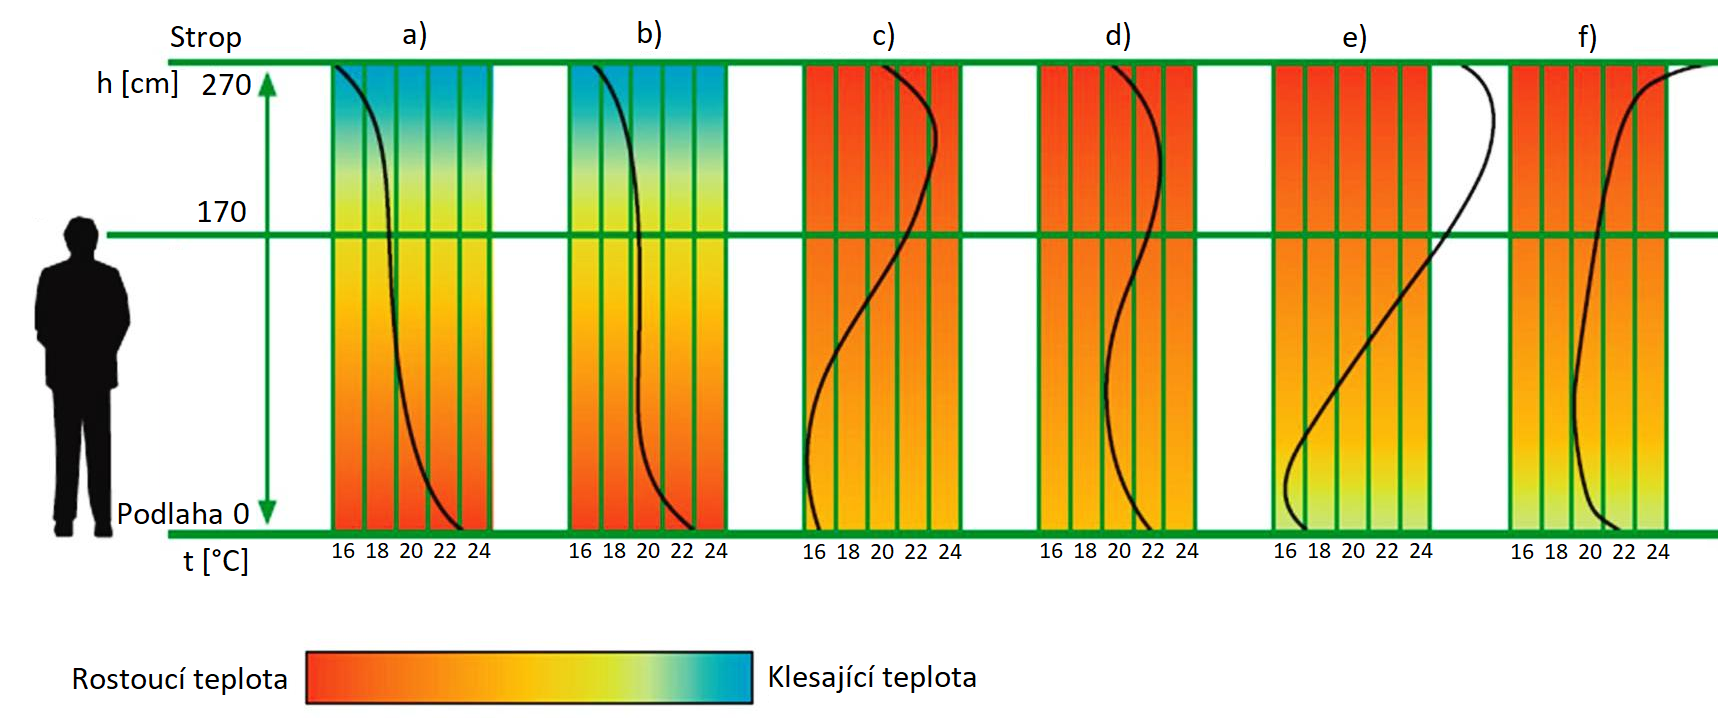
\includegraphics[width=\textwidth]{images/vertikalni-prubehy-teplot-pro-ruzne-druhy-vytapeni.png}}
\put(5,6){\scriptsize \sffamily Rostoucí teplota}
\put(161,6){\scriptsize \sffamily Klesající teplota}
\put(19,31){\scriptsize \sffamily t[°C]}
\put(15,132){\scriptsize \sffamily h[cm]}
\put(22,41){\fontsize{6}{6} \sffamily Podlaha}
\put(22,141){\fontsize{6}{6} \sffamily Strop}
\put(50,41){\scriptsize \sffamily 0}
\put(40,104){\scriptsize \sffamily 170}
\put(40,132){\scriptsize \sffamily 270}

\put(84,143){\scriptsize \sffamily a)}
\put(67,33){\fontsize{5}{5} \sffamily 16}
\put(74,33){\fontsize{5}{5} \sffamily 18}
\put(81,33){\fontsize{5}{5} \sffamily 20}
\put(88,33){\fontsize{5}{5} \sffamily 22}
\put(95,33){\fontsize{5}{5} \sffamily 24}

\put(134,143){\scriptsize \sffamily b)}
\put(117,33){\fontsize{5}{5} \sffamily 16}
\put(124,33){\fontsize{5}{5} \sffamily 18}
\put(131,33){\fontsize{5}{5} \sffamily 20}
\put(138,33){\fontsize{5}{5} \sffamily 22}
\put(145,33){\fontsize{5}{5} \sffamily 24}

\put(184,143){\scriptsize \sffamily c)}
\put(167,33){\fontsize{5}{5} \sffamily 16}
\put(174,33){\fontsize{5}{5} \sffamily 18}
\put(181,33){\fontsize{5}{5} \sffamily 20}
\put(188,33){\fontsize{5}{5} \sffamily 22}
\put(195,33){\fontsize{5}{5} \sffamily 24}

\put(234,143){\scriptsize \sffamily d)}
\put(217,33){\fontsize{5}{5} \sffamily 16}
\put(224,33){\fontsize{5}{5} \sffamily 18}
\put(231,33){\fontsize{5}{5} \sffamily 20}
\put(238,33){\fontsize{5}{5} \sffamily 22}
\put(245,33){\fontsize{5}{5} \sffamily 24}

\put(284,143){\scriptsize \sffamily e)}
\put(267,33){\fontsize{5}{5} \sffamily 16}
\put(274,33){\fontsize{5}{5} \sffamily 18}
\put(281,33){\fontsize{5}{5} \sffamily 20}
\put(288,33){\fontsize{5}{5} \sffamily 22}
\put(295,33){\fontsize{5}{5} \sffamily 24}

\put(334,143){\scriptsize \sffamily f)}
\put(317,33){\fontsize{5}{5} \sffamily 16}
\put(324,33){\fontsize{5}{5} \sffamily 18}
\put(331,33){\fontsize{5}{5} \sffamily 20}
\put(338,33){\fontsize{5}{5} \sffamily 22}
\put(345,33){\fontsize{5}{5} \sffamily 24}
\end{picture}
	 \caption[Vertikální průběh teploty vzduchu u podlahové vytápění.]{Vertikální průběh teploty vzduchu ve vytápěné místnosti při různém způsobu vytápění. \\ a) Ideální požadovaný průběh. b) Podlahové vytápění. c) Vytápění deskovými/článkovými otopnými tělesy (vnitřní stěna). d) Vytápění deskovými/článkovými otopnými tělesy (venkovní stěna). e) Konvektory. f) Stropní vytápění. Upraveno z \cite{vertikalni-prubehy-teplot-pro-ruzne-druhy-vytapeni}. }
	 \label{fig:vertikalni-prubehy-teplot-pro-ruzne-druhy-vytapeni}
\end{figure}

\hspace{5mm}

  \begin{figure}[H]
     \subfloat[Rozložení teplot při použití podlahové vytápění.\label{fig:rozlozeni-teplot-podlahove-vytapeni}]{
       \begin{overpic}[width=0.5\textwidth]{images/rozlozeni-teplot-podlahove-vytapeni.png}
         \put(20,10){\scriptsize \sffamily 22 °C}
         \put(65,50){\scriptsize \sffamily 20 °C}
         \put(8,115){\scriptsize \sffamily 17 °C}
         \put(155,90){\scriptsize \sffamily 18 °C}
       \end{overpic}
     }
     \subfloat[Rozložení teplot při použití deskových/článkových otopných těles. \label{fig:rozlozeni-teplot-radiatory}]{
       \begin{overpic}[width=0.5\textwidth]{images/rozlozeni-teplot-radiatory.png}
         \put(20,10){\scriptsize \sffamily 14 °C}
         \put(100,15){\scriptsize \sffamily 33 °C}
         \put(133,37){\scriptsize \sffamily 37 °C}
         \put(32,50){\scriptsize \sffamily 22 °C}
         \put(113,77){\scriptsize \sffamily 30 °C}
         \put(20,87){\scriptsize \sffamily 19 °C}
         \put(160,95){\scriptsize \sffamily 20 °C}
         \put(42,117){\scriptsize \sffamily 23 °C}
       \end{overpic}
     }
     \caption[Porovnání rozložení teplot při použití podlahové vytápění a deskových/článkových otopných těles.]{Porovnání rozložení teplot při použití podlahové vytápění a deskových/článkových otopných těles. Upraveno z \cite{rozlozeni-teplot-podlahove-vytapeni-a-radiatory}.}\label{fig:porovnani-rozlozeni-teplot}
   \end{figure}
   


\subsubsection{Výhody}

\begin{itemize}
  \item Je vhodné zejména tam, kde je nízkoteplotní zdroj tepla (tepelné čerpadlo, kondenzační kotel, solární panely, …).
  \item Větší užitný prostor (místo nezabírají otopná tělesa).
  \item Cirkulace vzduchu je nižší oproti deskovým/článkovým otopným tělesům, proto je víření prachu v~místnosti menší.
  \item Téměř rovnoměrná teplota místnosti.
\end{itemize}

\subsubsection{Nevýhody}

\begin{itemize}
  \item Zvýšené náklady na realizaci.
  \item Nezbytná pečlivá montáž a stavební dozor.
  \item Vyšší tepelná setrvačnost otopné soustavy.
  \item Vyšší nároky na řízení podlahové otopné plochy (zejména hlídání maximální vstupní otopné vody).
\end{itemize}

\section{Zónová regulace vytápění}

Význam zónové regulace vytápění spočívá v systému umožňující individuální vytápění v~jednotlivých místnostech (každá místnost nebo spojení více místností se označuje za zónu) na požadovanou teplotu.  Základ zónové regulace je centrální řídicí jednotka, která přijímá data od jednotlivých místností (zejména jejich aktuální teplotu) a dává povely do zařízení, které ovládá (otevírání/zavírání pohonů u jednotlivých otopných okruhů apod.). Přístup k~řídicí jednotce je nejčastěji pomocí displeje, webového rozhraní nebo jejich kombinace. V řídicí jednotce se dá celý systém vytápění nastavit (nastavení časových a teplotních programů pro jednotlivé zóny a mnohé další). 

Zónové systémy vytápění se rozdělují na dvě hlavní skupiny. První tvoří zónové systémy propojené pomocí vodičů a druhou skupinu tvoří bezdrátová technologie propojující centrální řídicí jednotku a jednotlivé zóny. 

Hlavní částí zónového systému je centrální řídící jednotka. Mezi další komponenty patří, nástěnné snímače vnitřní teploty, snímač venkovní teploty, termoelektrické pohony, elektronické regulátory otopných těles, reléová spínací jednotka. Mezi komponenty, které přispívají ke komfortu zónové regulace jako senzor intenzity slunečního záření, senzor rychlosti větru, různé spínací jednotky, jednotky pro ovládání žaluzií, moduly pro dálkové ovládání pomocí GSM a další.

\subsection{Principy zónové regulace vytápění}

Jak již bylo řečeno, základem celého systému je centrální řídicí jednotka. Další důležitou částí je zónový regulátor, který slouží pro ovládání komponentů, které jsou k zónovému regulátoru připojeny. Mezi hlavní komponenty, který zónový regulátor ovládá, jsou termoelektrické pohony. Termoelektrický pohon je podobný termostatické hlavici, která se nasazuje na deskové/článkové otopné těleso, ale je jej možné ovládat elektrickým napětím. Samotná regulace vytápění probíhá tak, že řídicí jednotka je propojena se zónovým regulátorem. K~zónovému regulátoru jsou připojeny jednotlivé nástěnné snímače prostorové teploty a termoelektrické pohony, které jsou nasazeny na termostatický ventilech otopných okruhů/těles. V centrální jednotce jsou nastaveny časové programy (různé požadované teploty pro různé časové úseky). Centrální jednotka posílá do zónového regulátoru požadované teploty pro všechny zóny. Tyto  teploty jsou v zónovém regulátoru porovnávány s aktuálními prostorovými teplotami měřenými nástěnnými jednotkami. V případě, že je prostorová teplota příslušné zóny nižší než požadovaná teplota (nastavená v centrální jednotce), ovládá zónový regulátor odpovídající pohon, který otevírá/zavírá daný ventil a umožňuje proudění otopné vody do otopného okruhu/tělesa, čím dochází ke změně teploty v místnosti. Pokud je připojen například kotel, je pak hořák kotle ovládán při požadavku vytápění v jakékoliv místnosti. Princip zónové regulace je zobrazen na obrázku \ref{fig:obecny-princip-zonove-regulace}.

Další možné zapojení může být takové, že jednotlivé nástěnné snímače prostorové teploty jsou přímo propojeny s centrální jednotkou, která následně podle časového programu posílá zónovému regulátoru požadavky na ovládání jednotlivých pohonů. 

\newpage
\begin{figure}[H]
    \centering
    \def\svgwidth{\columnwidth}
    \input{images/svg/obecny-princip-zonove-regulace.pdf_tex}
    \caption{Obecný princip zónové regulace vytápění.}
    \label{fig:obecny-princip-zonove-regulace}
\end{figure}

Mezi další ovládána zařízení při regulaci vytápění mohou být čerpadla, směšovací ventily zejména pro podlahové vytápění, kde je nutné udržovat teplotu otopné vody v daných mezích.

\subsection{Dostupné komerční řešení zónové regulace podlahového vytápění}

Optimální systém pro otopnou soustavu, kterou hodlám řídit z obrázku~\ref{fig:otopna-soustava-rez-domu}, se skládá z řízení ovládání kotle, spínání čerpadel v případě zatopení v~krbech a~následnou indikaci uživateli, jak je moc zásobník otopné vody naakumulovaný, dále z jednotlivých otopných okruhů (12 pohonů pro 9 zón) a~čerpadla podlahového vytápění. Pro zónovou regulaci se používá pouze patro.

\subsubsection{Elektrobock}
Česká firma Elektrobock nabízí bezdrátové řešení pro řízení podlahové vytápění. Systém řízení je zastřešené pod aplikaci PocketHome. Jednotlivé zařízení mohou fungovat samostatně bez nebo s centrální řídicí jednotkou. Tato centrální jednotka je zastřešené pod aplikaci PocketHome. Řídicí systém se skládá z centrální jednotky, nástěnných snímačů prostorové teploty pro jednotlivé místnosti a zónového regulátoru pro ovládání jednotlivých otopných okruhů (celkově je možné ovládat 9 zón) a oběhového čerpadla, dále je k dispozici zařízení pro zapínání/vypínání kotle nebo komunikace pomocí protokolu OpenTherm. Na obrázku \ref{fig:elektrobock-pocket-home} jsou zobrazena jednotlivá zařízení. Jistou nevýhodou může být bezdrátová komunikace na frekvenci 433,92 MHz, v případě delší vzdálenosti a především umístění na jiném patře centrální jednotky a nástěnných snímačů prostorové teploty, zónového regulátoru. Může docházet k problémům s komunikací, zejména pokud se jedná o~zástavbu z železobetonu, kde odrazivost a neprůchodnost signálu je poměrně značná. Jednotlivé prvky mohou pracovat samostatně bez centrální jednotky, na druhou stranu se tímto ztrácí přehled o celém systému a komfortu nastavování z jednoho místa. Systém se může spravovat pomocí PC (systém Windows) nebo pomocí chytrého telefonu/tabletu (systém Android, iOS). Systém počítá s jedním zdrojem tepla, tedy kotlem (elektrickým, plynovým, automatickým), neuvažuje se s otopnou soustavu, kde je začleněn např. krb s~tepelným výměníkem, jak z pohledu řízení čerpadel, tak i případnou indikaci o stavu naakumulovaní zásobníku s otopnou vodou. Problém bezdrátového, bateriového řešení je nutná výměna baterií po určité době.


\begin{figure}[H]

\centering
\begin{picture}(370,236)
\put(0,0){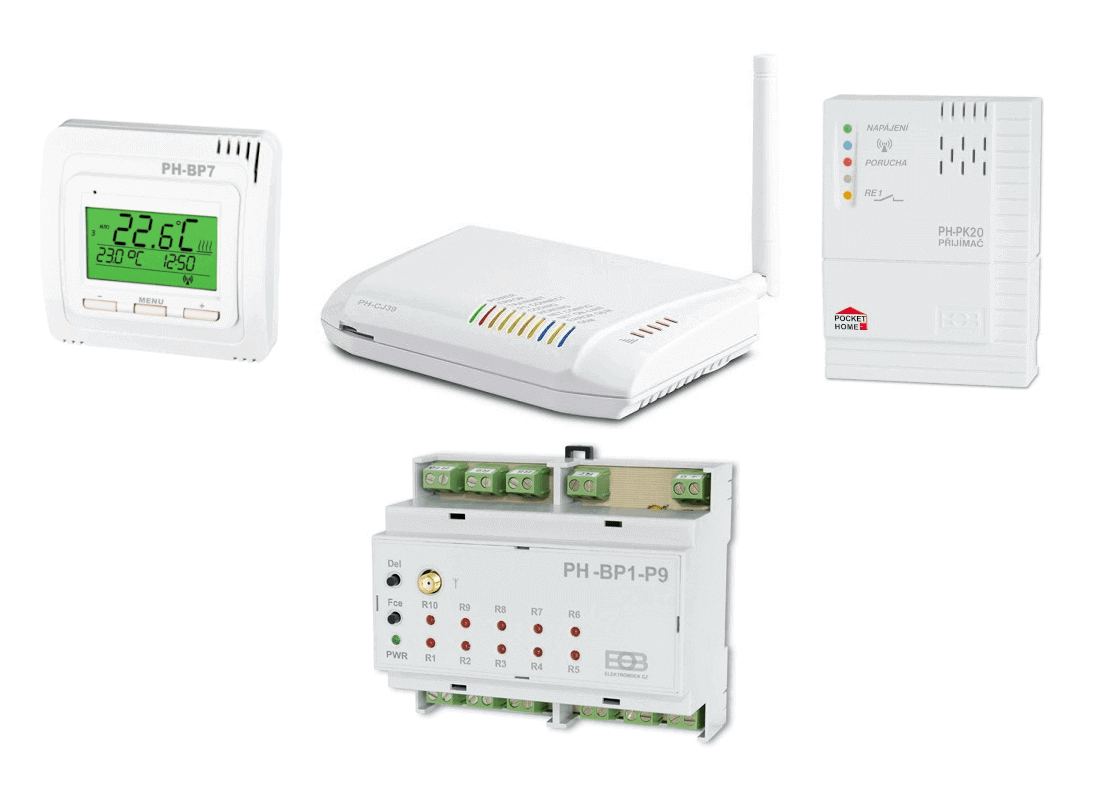
\includegraphics[width=\textwidth]{images/komercni-systemy/elektrobock-pocket-home/elektrobock-pocket-home.png}}
\put(50,226){\scriptsize \sffamily a)}
\put(180,190){\scriptsize \sffamily b)}
\put(305,235){\scriptsize \sffamily c)}
\put(180,8){\scriptsize \sffamily d)}
	 \caption[Jednotlivá zařízení systému Elektrobock PocketHome.]{Jednotlivá zařízení systému Elektrobock PocketHome. \\ 
	 a) Nástěnný snímač prostorové teploty. b) Centrální jednotka. c) Spínací jednotka kotle. d) Zónový regulátor. Upraveno z \cite{elektrobock-lokalni-termostat, elektrobock-centralni-jednotka, elektrobock-spinaci-jednotka-kotle, elektrobock-zonovy-regulator}.}
	 \label{fig:elektrobock-pocket-home}
\end{picture}

\end{figure}

\subsubsection{Honeywell}
Honeywell nabízí bezdrátový systém regulace podlahové vytápění. Systém řízení je zastřešené pod aplikaci Evohome. Skládá se z centrální jednotky s~dotykovým displejem, nástěnných snímačů prostorové teploty pro jednotlivé místnosti, zónového regulátoru pro ovládání jednotlivých otopných okruhů (celkově je možné ovládat 5 zón, s rozšiřovacím modulem je možné se dostat na 8 zón). Systém je možné rozšířit o dobíjení \acrshort{tuv} (\textit{\acrlong{tuv}}), pro sledování teploty na zásobníku je možné umístit teplotní čidlo, ze kterého je teplota odesílaná do centrální jednotky. Na obrázku \ref{fig:honeywell-evohome} jsou zobrazena jednotlivá zařízení systému. Systém však při dobíjení zásobníku TUV počítá se zdrojem tepla pouze s kotlem, takže v případě využití krbů s výměníkem nastává problém. V neposlední řadě umožňuje zapojit směšovací ventil pro optimální teplotu do podlahového topení. Systém je možné ovládat lokálně nebo řídit vzdáleně odkudkoliv, je zapotřebí zaregistrovat si účet a spárovat ho s  centrální jednotkou. Vzdálený server přijímá požadavky na změny režimů či nastavení teplot, a zasílá je do řídící jednotky. Server průběžně shromažďuje různá data o chování soustavy, a může je na základě žádosti poskytnout. Z~toho vyplývá, že pro lepší řízení a nastavení vytápění je nutné zřídit vzdálený přístup a samotné vyhodnocení a dání povelů, pak dochází na vzdálením serveru, nemáme moc pod kontrolou data a životnost takového systému do budoucnosti. Otázka je i při využití pouze lokálního režimu, zda regulace nepřichází o~výhody cloudového řešení. Problém bezdrátového řešení může být opět prostup signálu mezi zařízeními a centrální jednotkou (popsaný u předešlého systému), zejména prostup železobetonovými podlahami a to především při komunikace mezi centrální jednotkou umístěnou v patře a~komunikací mezi se zařízeními ve sklepě (nutný průchod dvěma podlahami) a je nutná výměna baterií v~zařízeních po určité době. Komunikace mezi zařízeními probíhá na frekvenci 868 MHz, připojení k centrální jednotce pomocí mobilní aplikace je pomocí WiFi.

\newpage

\begin{figure}[H]

\centering
\begin{picture}(370,300)
\put(0,0){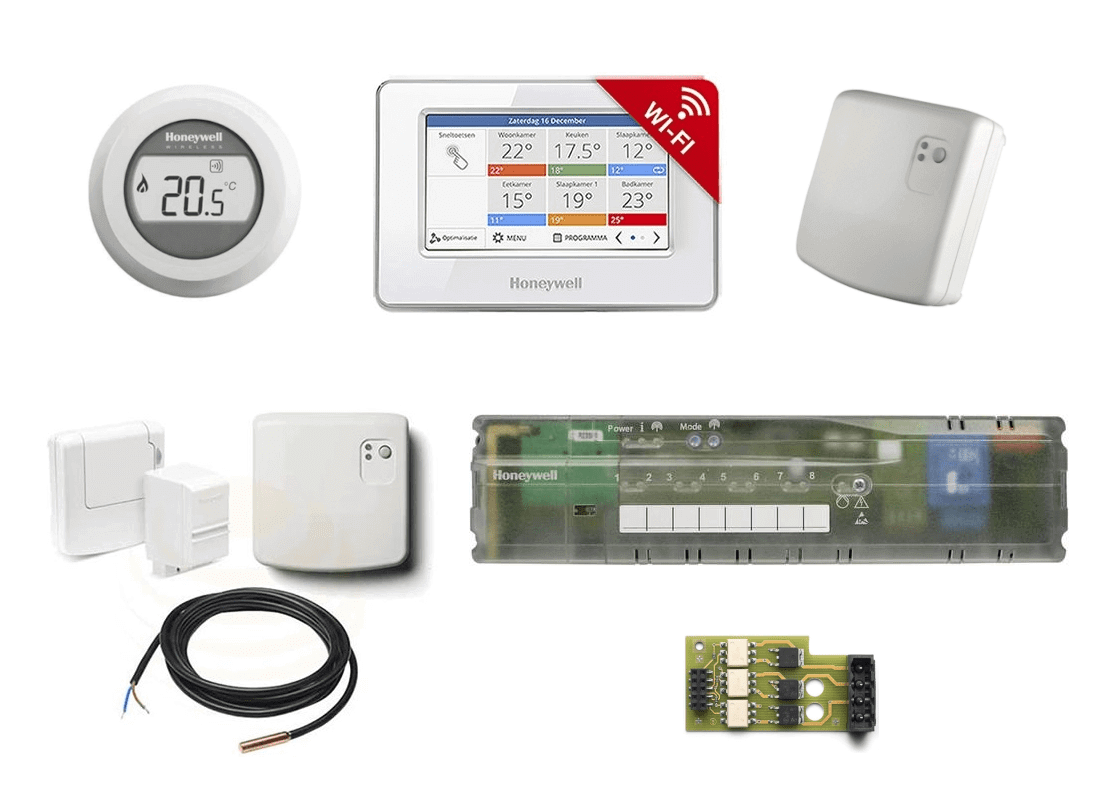
\includegraphics[width=\textwidth]{images/komercni-systemy/honeywell-evohome/honeywell-evohome.png}}
\put(60,240){\scriptsize \sffamily a)}
\put(180,240){\scriptsize \sffamily b)}
\put(305,240){\scriptsize \sffamily c)}
\put(60,130){\scriptsize \sffamily d)}
\put(250,130){\scriptsize \sffamily e)}
\put(250,57){\scriptsize \sffamily f)}
	 \caption[Jednotlivá zařízení systému Honeywell Evohome.]{Jednotlivá zařízení systému Honeywell Evohome.  \\
	 a) Nástěnný snímač prostorové teploty. b) Centrální jednotka. c) Spínací jednotka kotle. d) Řízení dobíjení TUV. e) Zónový regulátor. f) Rozšiřující modul pro  zónový regulátor. Upraveno z \cite{honeywell-lokalni-termostat, honeywell-centralni-jednotka, honeywell-spinaci-jednotka-kotle, honeywell-rizeni-dobijeni-tuv, honeywell-zonovy-regulator, honeywell-rozsirujici-modul-pro-zonovy-regulator}.}
	 \label{fig:honeywell-evohome}
\end{picture}

\end{figure}

\subsubsection{Danfoss}
Danfoss nabízí bezdrátový systém regulace podlahové vytápění. Systém řízení je zastřešený pod aplikaci Danfoss Link. Řídící systém se skládá z centrální jednotky s dotykovým displejem, nástěnných snímačů prostorové teploty  pro jednotlivé místnosti a zónového regulátoru pro ovládání jednotlivých otopných okruhů (celkově je možné ovládat 10 zón), oběhového čerpadla a řízení kotle. Na obrázku \ref{fig:danfoss-danfoss-link} jsou zobrazena jednotlivá zařízení systému. Vzdálené ovládání je umožněno přes mobilní aplikací pomocí cloudového řešení. Systém má absenci v řízení dobíjení TUV, respektive zásobníku na otopnou vodu a použití více zdrojů tepla (viz předchozích systémy). Opětovnými problémy může být šíření bezdrátového signálu mezi zařízeními (výrobce nabízí zesilovače/opakovače pro signál), problémy cloudového řešení a nutná výměna baterií po určité době (problémy více popsány u předešlých systémů). Komunikace mezi zařízeními probíhá na frekvenci 868 MHz.

\begin{figure}[H]
\centering
\begin{picture}(370,250)
\put(0,0){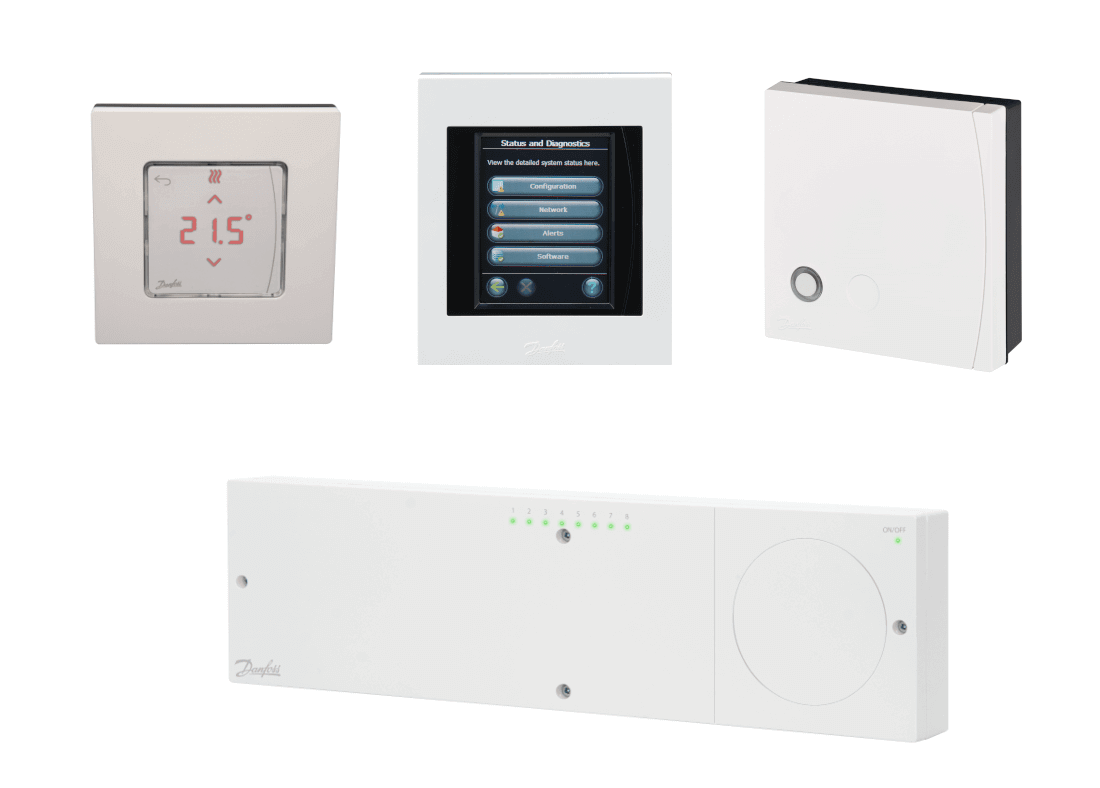
\includegraphics[width=\textwidth]{images/komercni-systemy/danfoss-danfoss-link/danfoss-danfoss-link.png}}
\put(60,242){\scriptsize \sffamily a)}
\put(180,242){\scriptsize \sffamily b)}
\put(305,242){\scriptsize \sffamily c)}
\put(180,102){\scriptsize \sffamily d)}
	 \caption[Jednotlivá zařízení systému Danfoss Danfoss Link.]{Jednotlivá zařízení systému Danfoss Danfoss Link. \\
	 a) Nástěnný snímač prostorové teploty. b) Centrální jednotka. c) Spínací jednotka kotle. d) Zónový regulátor. Upraveno z \cite{danfoss-lokalni-termostat, danfoss-centralni-jednotka, danfoss-zonovy-regulator, danfoss-spinaci-jednotka-kotle}.}
	 \label{fig:danfoss-danfoss-link}
\end{picture}

\end{figure}

Pokud shrnu hlavní nedostatky zmíněných systémů pro řízení podlahového vytápění, tak mezi ně patří bezdrátové ovládání, zejména tedy možný problém komunikace mezi centrální jednotkou a zařízeními. Výměna baterií v~zařízeních po určité době. Dále absence počítání s více zdroji tepla a~centrálním zásobníkem otopné vody, systém od firmy Honeywell umožňuje ovládaní ohřev pro TUV. Dalším možným nedostatkem může být cloudové řešení z pohledu dlouhodobé garance fungování služby, dále pak vzdálené ovládání neprobíhá přímo s centrální jednotkou, ale se vzdáleným serverem. Další zjištěním bylo, že všechny systémy jsou nabízeny jako bezdrátové, což je samozřejmě pochopitelné jak z pohledu jednoduchého nainstalování, již do stávajících staveb, kde s takovým systémem nebylo počítáno (zejména staré zástavby), též není nutné provádět žádné stavební úpravy. Pokud jsou nabízena drátová řešení není zde žádná centrální jednotka, ovládání probíhá přes drátové lokální termostaty připojené přímo na zónový regulátor, který následně ovládá jednotlivé otopné okruhy. Tabulka \ref{tab:srovnani-vlastnosti-jednotlivych-komercnich-systemu} zobrazuje přehled funkcí systémů zmíněné výše.


\begin{center}
\begin{table}[H]
\begin{threeparttable}
\begin{tabular}{|c||c|c|c|} \hline
\backslashbox{Funkce}{Systém}
& \thead{Elektrobock \\ (PocketHome)}  & \thead{Honeywell \\ (Evohome)} & \thead{Danfoss \\ (Danfoss Link)} \\


\hline
\thead{Napojení na více \\ zdrojů tepla} & Ne & Ne & Ne \\ 
\hline
\thead{Napojení na \\ centrální zásobník \\ otopné vody} & \multirow{2}{*}{Ne} & \multirow{2}{*}{Ne} & \multirow{2}{*}{Ne} \\ 
\hline
\thead{Ohřev TUV} & Ne & Ano & Ne \\ 
\hline
\thead{Bezdrátové$\slash$drátové \\ řešení} & Ano & Ano & Ano \\ 
\hline
\thead{Možnosti ovládání} & \makecell{PC \\ chytrý telefon} & \makecell{dotykový displej \\ chytrý telefon } & chytrý telefon \\ 
\hline
\thead{Cloudové řešení} & Ne & Ano & Ano \\ 
\hline
\makecell{Centrální \\ řídicí jednotka} & \makecell{(PH-CJ39-WIFI, 1×) \\ 3\,678 Kč}  & \makecell{(ATC928G3026,  1×) \\ 5\,994 Kč } & \makecell{(014G0288, 1×) \\ 8\,694 Kč }\\
Zónový regulátor & \makecell{(PH-BP1-P9, 1×) \\ 3\,388 Kč} & \makecell{(HCE80, 1×) \\ 5\,622 Kč} & \makecell{(088U1031, 1×) \\ 4\,299 Kč} \\
\makecell{Nástěnný snímač \\ prostorové teploty} & \makecell{(PH-BP7-V, 9×) \\ 9\,036 Kč} & \makecell{(T87RF2083, 9×) \\ 12\,141 Kč} & \makecell{(088U1081, 9×) \\ 19\,476 Kč} \\
Spínací jednotka kotle & \makecell{(PH-PK20, 1×) \\ 1\,498 Kč} & \makecell{(BDR91A1000, 1×) \\ 1\,100 Kč} & \makecell{(014G0272, 1×) \\ 2\,190 Kč}\\
Řízení dobíjení TUV & & \makecell{(ATF500DHW, 1×) \\ 3\,818 K}  & \\
\makecell{Rozšiřující modul \\ pro zónový regulátor}  & & \makecell{(HCS80, 1×) \\ 1 897 Kč} & \\
\thead{Celková cena \\ včetně DPH \tnote{a}} & 17\,600 Kč & 30\,572 Kč & 34\,659 Kč\\ 
\hline
\end{tabular}

	\begin{tablenotes}
    	\item[a] Ceny stanoveny ke dni 26. 11. 2020.
	\end{tablenotes}

\end{threeparttable}
 \caption{Srovnání funkcí jednotlivých komerčních systémů.}
 \label{tab:srovnani-vlastnosti-jednotlivych-komercnich-systemu}
 
\end{table}
\end{center}

V tabulce \ref{tab:srovnani-vlastnosti-jednotlivych-komercnich-systemu} chybí v části cen pohony pro ovládání jednotlivých otopných okruhů pomocí zónového regulátoru. Pro výše zmíněné systémy, zónový regulátor podporuje pohony na 230 V AC, pohony je možné koupit  přímo od daného výrobce nebo od jiného, na samotnou funkčnost to nemá vliv. Jediný rozdíl může být v pořizovací ceně, kde pro termoelektrické pohony je cena od 400 do 800 Kč, pro servopohony může být cena ještě vyšší. Celková cena za 12 pohonů se pohybuje v řádu jednotek tisíc. Někteří výrobci jako Danfoss nabízejí pro jejich systém zesilovače/opakovače signálu pro bezdrátový systém, v případě špatného průchodu signálu je možné zakoupit toto zařízení, ale nutné počítat s dalšími náklady navíc (řády jednotek tisíc). V případě, že systém neumí ovládat kotel pro dobíjení TUV, případně nesplňuje požadavky, které bychom chtěli, pak je nutné využít jiné řešení/systém, což se dále promítá do dalších nákladů a hlavně se jedná o nejednotnost jednoho systému.








\chapter{Návrh konceptu řídicího systému}

\section{Popis celkového konceptu}

Otopná soustava domu je zobrazena na obrázku \ref{fig:otopna-soustava-rez-domu}. Skládá v současné době pouze z jednoho zdroje tepla a to krbů v přízemí a v patře s teplovodními výměníky. Krby s teplovodním výměníkem slouží k ohřevu otopné vody proudící skrz vložku krbu, které dobíjí zásobník otopné vody. Na každém patře je rozdělovač podlahové topení s 12 otopnými okruhy, kde každý okruh se dá ovládat zvlášť (průtok otopné vody). Dále je zde čerpadlo a manuální trojcestný směšovací ventil pro nastavení optimální teploty do podlahového vytápění. Druhým zdrojem tepla je plynový kondenzační kotel, který není v~současnosti pořízen, nicméně se s ním počítá do budoucna. Bude sloužit k~ohřívání otopné vody, pokud nebudou využiti krby s teplovodním výměníkem, zejména v letním období pro ohřev TUV. Oba zdroje tepla jsou pro ohřívání otopné vody do centrálního zásobníku (objem je 1 500 l). Kde je přibližně v jedné horní třetině výšky zásobníku umístěna nádoba TUV (objem je 120~l). Navržený systém řídí ovládání čerpadel u rozdělovačů podlahové topení, čerpadel pro krby s výměníkem a pohonů pro jednotlivé okruhy podlahové vytápění. K ovládání čerpadel, otopných okruhů dochází při požadavku topení nebo pokud dojde k topení v krbech. Řízení podlahového vytápění respektive pohonů dochází pouze v patře na základě požadavku majitele. Celkově v~patře se nachází více obytných místností.


\begin{figure}[H]
    \centering
    \def\svgwidth{\columnwidth}
    \input{images/svg/otopna-soustava-rez-domu.pdf_tex}
    \caption{Otopná soustava v domě.}
    \label{fig:otopna-soustava-rez-domu}
\end{figure}

\subsection{Hardwarová část}

Centrální jednotka je jednodeskový počítač s periferiemi jako ethernetový port, \acrshort{usb} (\textit{\acrlong{usb}}), univerzálními vstupy/výstupy, případně s alternativní funkcí pinů jako sběrnice \acrshort{i2c} (\textit{\acrlong{i2c}}) nebo dalšími typy periferií. Dále by měla disponovat dostatečnou velikostí \acrshort{ram} (\textit{\acrlong{ram}}) pamětí a relativně výkonným procesorem pro snadné zpracování vstupní/výstupních dat či povelů.

Bezdrátové nástěnné snímače prostorové teploty jsou napájeny z lokálních síťových adaptérů, každý modul má své napájení. Nástěnný snímač prostorové teploty se skládá z displeje pro zobrazení aktuální a požadované teploty a~dalších nastavení. Dále ze tří tlačítek pro vstup do menu a tlačítek pro zvýšení/snížení požadované teploty a teplotního senzoru. Komunikace s~centrální jednotkou je zajištěna pomocí WiFi modulu skrz WiFi router.

Kabelové nástěnné snímače prostorové teploty jsou napájeny pomocí switche s POE. Nástěnný snímač prostorové teploty se skládá z displeje pro zobrazení aktuální a požadované teploty a dalších nastavení. Dále ze tří tlačítek pro vstup do menu a tlačítek pro zvýšení/snížení požadované teploty a teplotního senzoru. Komunikace s centrální jednotkou je zajištěna skrz zmíněného switche.

Indikátor stavů je propojen přímo s centrální jednotkou, skládá z části indikující stavy pomocí \acrshort{led} (\textit{\acrlong{led}}) pro jednotlivé teploty měřené v zásobníku otopné vody rozmístěné v jednotlivých částech nádrže. Dále je zde sběrnice pro komunikaci \acrshort{lcd} (\textit{\acrlong{lcd}}) displejem a~centrální jednotkou pro zobrazení teplot ze zásobníku, respektive dvou teplot ze spodní části. LED diody a LCD displej jsou umístěny u krbů v~každém patře.

Spínací jednotka se skládá z relé modulů pro ovládání jednotlivých čerpadel pro oběh otopné vody do otopných okruhů podlahové vytápění v jednotlivých patrech. Dále jsou zde ovládána čerpadla pro cirkulaci vody z krbových výměníků. V neposlední řadě je zde případné ovládání plynové kondenzačního kotle.

Zónový regulátor je umístěn v daném patře v rozdělovači pro jednotlivé otopné okruhy. Komunikace mezi zónovým regulátorem a centrální jednotkou je pomocí sběrnice. Zónový regulátor ovládá jednotlivé pohony pomocí \acrshort{pwm} (\textit{\acrlong{pwm}}) signálu. Pohony jsou přímo připojené na zónový regulátor.

Síťové prvky se skládají z centrálního switche, switche s \acrshort{poe} (\textit{\acrlong{poe}}) a domácího WiFi routeru. Centrální switch sdružuje veškerou komunikaci jak z kabelových nástěnných snímačů prostorové teploty, tak i bezdrátových. Bezdrátové nástěnné snímače prostorové teploty jsou připojeny pomocí WiFi routeru a~ten následně do centrální switche, který přepojuje komunikaci do centrální jednotky. Kabelové nástěnné snímače prostorové teploty jsou připojeny přes switch s POE, který zařízení napájí a přeposílá komunikaci do centrálního switche, který přepojuje komunikaci do centrální jednotky.

Teplotní senzory v zásobníku otopné vody jsou rozmístěné ve třech částech zásobníku (horní, střední a spodní část). Dále jsou teplotní senzory na kouřovodech u jednotlivých krbů pro detekci topení. Všechny senzory jsou napojeny na jednu sběrnici.

Výše popsaný hardwarový koncept je nakreslen na obrázku \ref{fig:navrh-hardwarove-casti}.

\begin{figure}[H]
    \centering
    \def\svgwidth{\columnwidth}
    \input{images/svg/navrh-hardwarove-casti.pdf_tex}
    \caption{ Návrh hardwarové části systému.}
    \label{fig:navrh-hardwarove-casti}
\end{figure}

\subsubsection{Teplotní čidla}
Jak bylo zmíněno výše, teplotní čidla jsou potřebná na snímání teplot na kouřovodech krbů pro následné sepnutí oběhového čerpadla. Teplota na kouřovodech se může dosáhnout až 300 °C (optimální teplota se však pohybuje přibližně mezi 120 °C až 240 °C, kdy je nejvyšší účinnost kamen a hoření paliva), proto je nutné zvolit takové čidlo, které je na tyto teploty vhodné. Mezi takové teplotní čidlo patří odporový teplotní senzor (teplotní rozsahy od -240~°C až 600 °C) nebo termočlánek (teplotní rozsahy od -260 °C až 2~300~°C). Pro zjištění teploty není nutná velmi velká přesnost, citlivost, jistým požadavkem je robustnost čidla (nejen ochrana čidla, ale i přívodních kabelů), vzhledem k umístění u krbu, kde je dosahováno vyšších teplot.

%Princip termočlánku spočívá v Seebeckově efektu, jsou-li spojeny dva vodiče z různých kovů, tak v místě spojení je generováno napětí. Velikost napětí je závislá na vnější teplotě a materiálu článku. Linearita výstupního napětí článku je závislá na typu termočlánku a rozsahu teplot.

Další teplotní senzory jsou nutná pro nástěnné teplotní snímače prostorové teploty pro každou místnost, zásobník otopné vody a venkovní čidlo. Teplotní rozsah těchto čidel nemusí být tak vysoký jako u měření teplot na kouřovodech. Teplotní rozsah stačí v řádů desítek stupňů jak pro kladné, tak i záporné hodnoty teploty. %Vzhledem ke vzdálenostem teplotních čidel a centrální jednotky bude lepší zvolit digitální teplotní čidla, které výslednou změřenou teplotu zpracuje pošle po sběrnici v digitální podobě. Není pak nutná další elektronika pro zpracování hodnot teploty jako například u termočlánku či teplotně odporového čidla.

\subsection{Komunikační část}

Komunikace mezi centrální řídicí jednotkou a bezdrátovými i kabelovými nástěnnými snímači prostorové teploty jsou zajištěny pomocí protokolu MQTT. Centrální jednotka dostává informace z jednotlivých nástěnných snímačů prostorové teploty, zároveň je možné některé parametry nastavovat přímo přes centrální jednotku, která následně dané nastavení pošle do daných zařízení.

Indikátor stavů komunikuje s centrální jednotkou pomocí sběrnice I$^2$C pro zobrazení hodnot na LCD displeji. Zároveň je zde přímé připojení na vstupní/výstupní piny centrální jednotky pro ovládání indikačních LED diod.

Spínací jednotka je přímo připojena s centrální jednotkou pro spínání daných čerpadel pro podlahové vytápění, čerpadel pro krbové výměníky a~kondenzačního plynového kotle.

Zónový regulátor komunikuje s centrální jednotkou pomocí I$^2$C sběrnice, následné ovládání pohonů pro otopné okruhy je přímo zónovým regulátorem.

Teplotní senzory umístěné v zásobníku otopné vody a na kouřovodech krbů komunikují s centrální jednotkou pomocí 1-Wire sběrnice.

Výše popsaný komunikační koncept je nakreslen na obrázku \ref{fig:navrh-softwarove-casti}.

\begin{figure}[H]
    \centering
    \def\svgwidth{\columnwidth}
    \input{images/svg/navrh-softwarove-casti.pdf_tex}
    \caption{Návrh komunikační části systému.}
    \label{fig:navrh-softwarove-casti}
\end{figure}

\subsubsection{MQTT protokol}

\acrshort{mqtt} (\textit{\acrlong{mqtt}}) je jednoduchý a nenáročný \acrshort{m2m} (\textit{\acrlong{m2m}})/„Internet of Things“ komunikační protokol. Protokol je založen na principu předávání zpráv mezi klienty přes centrální server (broker). Centrální server přijímá zprávy od poskytovatele zprávy (tzv. publisher), které následně předává k přečtení čtenářům, kteří tuto zprávu odebírají (tzv. subscribers). Poskytovatel zprávy obvykle představuje nějaký senzor či měřící jednotku, která vysílá naměřeného hodnoty na centrální server, zatímco odběratel obvykle tvoří nějaká řídící jednotka, která hodnoty odebírá (přijímá) a dále s nimi pracuje nebo je zobrazuje.

Přenášené zprávy jsou tříděny do témat (tzv. topic). Každá zpráva patří právě do jednoho tématu, přičemž témata definuje přímo poskytovatel zprávy. Odběratel pak musí předem znát jméno (označení) tématu, aby se mohlo přihlásit u~centrálního serveru k jeho odběru. Odběratel nemusí znát umístění ani komunikační adresu poskytovatele zprávy. Musí jen znát komunikační adresu (umístění) centrální serveru. Témata jsou hierarchická a oddělená lomítky. Příklad struktury tématu:~„dum/patro/loznice/sensor/teplota“, lze tak přehledně roztřídit jednotlivá umístění zařízení a případné rozšiřování systému je pak snadné. Příklad schématu komunikace a struktury témat je zobrazen na obrázku \ref{fig:mqtt-protokol}.
\setnowidow[2]

\begin{figure}[H]
    \centering
    \def\svgwidth{\columnwidth}
    \input{images/svg/mqtt-protokol.pdf_tex}
    \caption[Základní funkční schéma MQTT komunikace.]{Základní funkční schéma MQTT komunikace. Příklad přenosu hodnot do koncových zařízení. Znak \# nahrazuje jednu či více úrovní, budou přijímány odběrateli všechny zprávy tykající se prvního patra domu.}
    \label{fig:mqtt-protokol}
\end{figure}

Obsahem zprávy není přesně definován. Nejčastěji se používá formát (způsob zápisu) dat \acrshort{json} (\textit{\acrlong{json}}), \acrshort{bjson} (\textit{\acrlong{bjson}}) nebo textové zprávy. Velikost zprávy je pak v aktuální verzi protokolu omezena na necelých 256 MB, ale vzhledem k využití „Internet of~Things“ bývá většina zpráv mnohem menší.

Protokol MQTT popisuje jen samotný popis struktury přenášených zpráv, ale nedefinuje způsob přenosu. K tomu se využívá \acrshort{tcp/ip} (\textit{\acrlong{tcp/ip}}) protokol. Protokol definuje tři úrovně potvrzování zpráv \acrshort{qos} (\textit{\acrlong{qos}}). QoS 0 – zpráva je odeslána bez potvrzení a není zaručeno její doručení. QoS 1 – poskytovatel zprávy zprávu odešle a přes centrální server je od odběratelů posláno potvrzení, centrální server může poslat potvrzení, aniž by měl potvrzení od všech odběratelů (závisí na implementaci). QoS 2 – poskytovatel zprávu odešle, centrální server pošle poskytovateli zprávy potvrzení o přijetí, na kterou poskytovatel zprávy odpoví potvrzením. Centrální server zprávu smaže a potvrdí zprávou, čímž je komunikace mezi poskytovatelem zprávy a~centrálním serverem uzavřena. Tato komunikace probíhá i mezi centrálním serverem a~odběrateli.


V přihlašovací sekvenci se využívá identifikace klienta pomocí ID a pak volitelně i pomocí uživatelské jména a hesla. MQTT díky podpoře \acrshort{ssl} (\textit{\acrlong{ssl}})/\acrshort{tls} (\textit{\acrlong{tls}}) umožňuje přihlášení pomocí klientského SSL certifikátu.
\setnowidow[2]
\subsubsection{I$^2$C sběrnice}
Jedná se o sériovou, synchronní a poloduplexní sběrnici. Komunikace probíhá na dvou vodičích, jeden tvoří hodinový vodič \acrshort{scl} (\textit{\acrlong{scl}}) a~datový vodič \acrshort{sda} (\textit{\acrlong{sda}}). Vodiče jsou sdílené mezi připojenými zařízeními, proto je možné aby kdokoliv komunikoval s kýmkoliv (komunikace je v této konfiguraci náročnější na zpracování). Typické zapojení sběrnice je v konfiguraci jeden master, který veškerou komunikaci řídí, a několik zařízení slave, viz obrázek \ref{fig:i2c-sbernice}. Nicméně existuje varianta s více mastery, existuje sada pravidel, jak se musí chovat, aby mohly na sběrnici pracovat společně a neovlivňovaly se. Na vodičích SCL a SDA je připojen pull-up rezistor (R), v neutrálním stavu je na vodičích log. 1. Připojená zařízení po sběrnici komunikují pomocí otevřeného kolektoru (mohou sběrnici stáhnout k zemi (log. 0), po odpojení je na sběrnici opět log. 1).

\begin{figure}[H]
    \centering
    \def\svgwidth{\columnwidth}
    \input{images/svg/i2c-sbernice.pdf_tex}
    \caption[Zapojení I$^2$C sběrnice.]{Zapojení I$^2$C sběrnice. Jedno zařízení pracuje v režimu master, ostatní zařízení v režimu slave.}
    \label{fig:i2c-sbernice}
\end{figure}

Komunikace vždy začíná START sekvencí (na SDA se vygeneruje sestupná hrana, na SCL je držena log. 1) a končí STOP sekvencí (na SDA se vygeneruje vzestupná hrana, na SCL je držena log.). SDA nesmí nikdy měnit svojí hodnotu, když je SCL v log. 1.  Přenos jednoho bitu zprávy probíhá, takže SCL je v log. 0, změní vysílač hodnotu SDA na takovou, jakou potřebuje. Poté nastaví SCL do log. 1. Se vzestupnou hranou pak přijímač čte hodnotu na SDA. Vysílač opět vrátí SCL do log. 0 a celý proces se opakuje s dalším bitem zprávy. Zpráva se skládá z 9 bitů. Prvních 8 bitů je datových a devátý bit je potvrzovací (log. 0 pro potvrzení nebo log. 1 a vysílač z toho vyrozumí, že zpráva není potvrzená). Nejednodušší tvar zprávy se skládá ze START sekvence, 8 bitů, potvrzovací devátý bit a STOP sekvence. Prvních 7 bitů po START sekvenci tvoří adresu zařízení (každý slave má unikátní adresu, jinak dojde ke kolizi) a osmý bit rozhoduje o směru toku dat (zda se bude zapisovat log. 1 či číst log. 0), každý byte se potvrzuje devátým bitem, buď potvrzuje slave, když master posílá data nebo naopak master potvrzuje, když posílá slave. Tak to se potvrzuje až na poslední byte, tím se zařízení dozví, že komunikace končí a~má uvolnit SDA linku. Poté se odešle STOP sekvence. Zobrazení komunikace je na obrázku \ref{fig:i2c-sbernice-datova-komunikace-7bit-adresa}.

\begin{figure}[H]
    \centering
    \def\svgwidth{\columnwidth}
    \input{images/svg/i2c-sbernice-datova-komunikace-7bit-adresa.pdf_tex}
    \caption[Příklad I$^2$C datové komunikace se 7-bitovou adresací.]{Příklad I$^2$C datové komunikace se 7-bitovou adresací. Upraveno z~\cite{i2c-sbernice-datovy-paket-7bit-adresa}.}
    \label{fig:i2c-sbernice-datova-komunikace-7bit-adresa}
\end{figure}

Adresace je možná pomocí 7 bitů (128 unikátních adres, číslo je však poníženo ještě o speciální adresy, např. broadcast adresa apod.) nebo 10 bitů (1024 unikátních adres), zde se pak adresy přenáší ve dvou bytech (pro první byte se používá vyhrazená adresa, kde jsou uloženy dva nejvyšší bity adresy, v~druhém bytu je dolních osm bitů adresy).

Podle verze sběrnice je frekvenci SCL 100 kHz, 400 kHz, 1 MHz nebo až 3,4 MHz. Rychlost je pak přizpůsobena nejpomalejšímu zařízení na sběrnici. Pull-up rezistory jsou v řádech jednotek kiloohmů, s rostoucí frekvencí nebo delší vzdálenosti sběrnice se jejich velikosti volí menší.




\subsubsection{1-Wire sběrnice}
Jedná se o sériovou, asynchronní a poloduplexní sběrnici. Komunikace probíhá na jednom vodiči, dalšími vodiči jsou napájení (V$_{DD}$) a zem (GND) to je v~případě konfigurace pomocí tří vodičů (obrázek \ref{fig:1-wire-sbernice-tri-vodice}), další typ konfigurace sběrnice je pomocí jen dvou vodičů, kde napájení a komunikace probíhá na jednom vodiči, druhý vodič je zem (obrázek \ref{fig:1-wire-sbernice-dva-vodice}), během neutrálního stavu na sběrnici (log. 1) dochází k~nabíjení interního kondenzátoru, který se následně chová jako zdroj energie při log. 0 na sběrnici (komunikace), v~tomto režimu je nutné splnit vhodné podmínky pro napájení a časování pro správnou komunikaci. Sběrnice se skládá z řídícího obvodu master a jednoho či více připojených zařízení slave. Na vodiči data je připojen pull-up rezistor (R), v~neutrálním stavu je na vodiči log. 1. Připojená zařízení po sběrnici komunikují pomocí otevřeného kolektoru (mohou sběrnici stáhnout k zemi (log. 0), po odpojení je na sběrnici opět log. 1).

Komunikaci zahajuje vždy master reset pulsem. Dojde ke vygenerování sestupné hrany na datovém vodiči na log. 0 po dobu minimálně 480 µs. Pak master sběrnici uvolní (opět se objeví log. 1) a naslouchá. Pokud je na sběrnici připojené zařízení, tak detekuje tuto vzestupnou hranu a po prodlevě (15–60~µs) vygeneruje na sběrnici po dobu 60–240 µs log. 0. Průběh komunikace je zobrazen na obrázku \ref{fig:1-wire-reset-vysilani-prijem-dat}a. Pokud se zařízení správně ohlásí, může master začít vysílat a přijímat data, která jsou vysílána v tzv. time slotech. Slot je dlouhý 60–120~µs a během jednoho slotu je vyslán nebo přijat jeden bit informace. Mezi jednotlivými sloty musí být minimálně 1 µs mezera, kdy je sběrnice v klidu. 

Existují 4 ruhy slotů: zápis 1, zápis 0, čtení 1 a čtení 0. Sloty pro zápis slouží k tomu, aby master vyslal data do zařízení. Zápis 1 probíhá tak, že master vygeneruje na sběrnici log. 0 minimálně na 1 µs a nejpozději do 15 µs od začátku ji opět uvolní a ponechá volnou. Zápis 0 probíhá tak, že master vygeneruje na sběrnici log. 0 a ponechá ji tak po celý slot, tedy minimálně 60~µs. Zařízení vzorkuje stav na datovém vodiči zhruba 30 µs po začátek time slotu. Průběh komunikace je zobrazena na obrázku \ref{fig:1-wire-reset-vysilani-prijem-dat}b.

Čtecí sloty inicializuje master, vygeneruje na sběrnici log. 0 na minimálně 1~µs a~opět ji uvolní. Po tomto zahájení může zařízení vyslat 1 bit, ponechá sběrnici v~klidu (log. 1) nebo je vygeneruje na log. 0. Průběh komunikace je zobrazena na obrázku \ref{fig:1-wire-reset-vysilani-prijem-dat}c.

Každé zařízení má v sobě paměť \acrshort{rom} (\textit{\acrlong{rom}}), která obsahuje 64bitové unikátní číslo, které slouží k odlišení jednotlivých zařízení na sběrnici. Po RESET pulsu je třeba vyslat příkaz Match ROM, pak 64bitový kód zařízení, se kterým se má pracovat, a teprve poté se posílá příkaz.


\begin{figure}[H]
    \centering
    \def\svgwidth{\columnwidth}
    \input{images/svg/1-wire-sbernice-tri-vodice.pdf_tex}
    \caption{Zapojení 1-Wire sběrnice ve trojvodičovém provedení.}
    \label{fig:1-wire-sbernice-tri-vodice}
\end{figure}

\begin{figure}[H]
    \centering
    \def\svgwidth{\columnwidth}
    \input{images/svg/1-wire-sbernice-dva-vodice.pdf_tex}
    \caption{Zapojení 1-Wire sběrnice ve dvouvodičovém provedení.}
    \label{fig:1-wire-sbernice-dva-vodice}
\end{figure}

\newpage

\begin{figure}[H]
    \centering
    \def\svgwidth{0.99\columnwidth}
    \input{images/svg/1-wire-reset-vysilani-prijem-dat.pdf_tex}
    \caption[Průběhy na sběrnici 1-Wire.]{Průběhy na sběrnici 1-Wire.
    a) Reset. b) Zápis dat. c) Čtení dat. Upraveno z \cite{1-wire-sbernice-prubehy}.}
    \label{fig:1-wire-reset-vysilani-prijem-dat}
\end{figure}

\section{Řídicí systém}
V současné době existuje poměrně dost open-source projektů pro monitorování a ovládání domácí automatizaci. Do které lze zařadit inteligentní řízení vytápění. Mezi velké projekty lze jmenovat systém Home Assistant a OpenHab. Oba jsi jsou poměrně podobní, liší programovacím jazykem, který je použit pro jejich systémové jádro, dále syntaxí pro zápis automatizací, množstvím integrovatelných zařízení (vytvořené \acrshort{api} (\textit{\acrlong{api}}) pro snadné spárování), vydáváním aktualizací, složitostí vytváření či přidávání zařízení do systému, přehlednou a dostupnou dokumentací a uživatelskou základnou, případně dalšími vlastnostmi. Na základě zkušenosti se systémem Home Assistant jak z pohledu dobré zkušenosti ze strany komunity, široké nabídky možnosti nastavení a relativně rychlou tvorbou automatizace jsem tento systém zvolil pro řízení vytápění rodinného domu.

\subsection{Home Assistant}
Home Assistant (dále jen \acrshort{ha}) je systém naprogramovaný v jazyce Python 3 a~podporuje mnoho technologií používaných v oblasti domácí automatizace. HA podporuje několik stovek zařízení či služeb (obecně komponent) od desítek velkých firem. Přesněji sdružuje jejich společné ovládání a vzájemnou propojenost automatizací. Vše je tak na jednom místě a možné ovládat přes jednoduché grafické rozhraní.

Všechna data jsou uložena na vlastním úložišti, tedy vlastním počítači, nasu, Raspberry Pi apod. Není tedy potřeba zakládat účet pro využívání služeb (některé služby však potřebují internetové připojení pro stahování informací např. předpověď počasí) a posílat data třetím stranám.

Systém se skládá ze samotné aplikace HA a z operačního systému na kterém HA běží. HA je možné nainstalovat na systém Linux, Windows, macOS. Též je přímá oficiální podpora pro Raspberry Pi, Asus Tinkerboard, Odroid a~Intel NUC, nicméně funkčnost lze najít i pro jiná zařízení. Existují čtyři varianty instalace systému, liší se nutnými zkušenostmi pro správu HA tak i~operačního systému, možnostmi správy aktualizací či obnovování, vracení nastavení, dále způsoby zálohování, možnostmi operačního systému (zda je předinstalován omezený OS nebo se jedná o plnohodnotnou verzi) v~neposlední řadě, zda je využit kontejner Docker či je HA nainstalován přímo v operačním systému, nebo lépe při využití virtuálního prostředí.

\subsubsection{Architektura Home Assistantu}
Obecně není stanoven otevřený standard pro komunikaci inteligentních zařízení. Tato skutečnost zamezuje vzájemnou komunikaci mezi zařízeními a~především většina zařízení není určena k řízení jiných zařízení. V HA se takové zařízení, která spravuje všechny ostatní nazývá \textbf{rozbočovač}.

Minimum, co by rozbočovač měl umět, je sledovat stav připojených zařízení a schopnost je řídit. Například u světel nás zajímá informace, zda jsou rozsvícená či nikoliv a umožnit změnit jejich stav. U senzoru sledujeme jeho hodnotu. Rozbočovač s~těmito možnostmi umožňuje \textbf{řízení domácnosti}.

Jistým krokem k domácí automatizaci je spuštění \textbf{uživatelsky nadefinovaných nastavení} na základě informací z domácí vrstvy řízení (například zatažení žaluzií při nadměrném osvícení slunečními paprsky). Rozbočovač s~těmito schopnostmi je schopný \textbf{domácí automatizace}.

Poslední kategorie, která je stále v budoucnu se nazývá \textbf{chytrý domov}. Samoučící a adaptivní systém, který rozhoduje, která událost by měla ovlivnit jiná zařízení.

Výše popsaný přehled řízení domácí automatizace HA je na obrázku \ref{fig:ha-prehled-domaci-autmatizace}.


\begin{figure}[H]
    \centering
    \def\svgwidth{\columnwidth}
    \input{images/svg/ha-prehled-domaci-autmatizace.pdf_tex}
    \caption[Přehled řízení domácí automatizace HA.]{Přehled řízení domácí automatizace HA. Upraveno z \cite{home-assistant-architektura}.}
    \label{fig:ha-prehled-domaci-autmatizace}
\end{figure}

\subsubsection{Jádro architektury Home Assistant}
Jádro HA odpovídá za řízení domácnosti. Skládá ze čtyř části, které to umožňují (obrázek \ref{fig:ha-jadro-architektury}):

\begin{itemize}
\item Sběrnice událostí – umožňuje vyvolání a poslech událostí – „srdce“ HA.
\item Stavový stroj – sleduje stav zařízení a spustí \textbf{změnu stavu} událostí, pokud došlo ke změně.
\item  Registr služeb – poslouchá sběrnici událostí pro \textbf{volání služby} událostí a umožňuje jinému kódu registrovat služby.
\item Časovač – posílá události \textbf{změny času} každou jednu sekundu na sběrnici událostí.
\end{itemize}

\begin{figure}[H]
    \centering
    \def\svgwidth{\columnwidth}
    \input{images/svg/ha-jadro-architektury.pdf_tex}
    \caption[Jádro architektury HA.]{Jádro architektury HA. Upraveno z \cite{home-assistant-architektura}.}
    \label{fig:ha-jadro-architektury}
\end{figure}

\subsubsection{Architektury komponent}
HA je možné rozšiřovat přes tzv. komponenty. Každá komponenta odpovídá za určitou oblast v rámci HA. Komponenty mohou poslat spouštěcí události, nabízet služby a řídit/měnit stavy. Komponenty jsou napsány v Pythonu. Sám HA nabízí několik stovek takovýchto komponent k použití. Znázornění využití komponent je na obrázku \ref{fig:ha-architektura-komponent}.

\begin{figure}[H]
    \centering
    \def\svgwidth{\columnwidth}
    \input{images/svg/ha-architektura-komponent.pdf_tex}
    \caption[Znázornění využití komponent v HA.]{Znázornění využití komponent v HA. Upraveno z \cite{home-assistant-architektura}.}
    \label{fig:ha-architektura-komponent}
\end{figure}

Jsou zde dva typy komponent. První typ, které interagují se zařízeními „Internet of Things“ (například inteligentní žárovky). Druhý typem jsou komponenty, které reagují na událost ke kterým dojde v~HA (například nastavená automatizace).


\subsection{Inteligentní část systému}
Pro co největší využití centrálního řízení podlahového vytápění je vhodné využít různé metody pro její optimalizaci, což se následně promítne do nákladů energie, taktéž i do teplotního komfortu uživatelů. Velmi častá situace je, že domy jsou vytápěny podle momentální teploty. Toto řešení není ideální, zejména v zateplených domech, případně s podlahovým topením. Problémem jsou hlavně podzimní a zimní dny, kdy teplota nad ránem prudce klesne. Reakce vytápěcího systému je poměrně rychlá a začne přitápět. Vzhledem k~setrvačnosti otopné soustavy a to především u podlahového topení dojde k~pomalé teplotní změně, než se dané nastaví projeví, ranní mrazík mezitím zmizí. Opačný problém může nastat odpoledne, kdy začnou sluneční paprsky pražit do oken, čímž máme nepříjemně přetopeno. Výsledkem je nepříjemný uživatelský komfort a zbytečná platba za energie.

Jednou z metod je využití předpovědi počasí, kdy dopředu víme teplotní předpověď, kterou můžeme začlenit do teplotních programů (časově nastavený úsek pro vytápění) definované uživatel a na základě  předpovědi se rozhodnout, zda je nutné v místnosti přitápět dříve v případě snížení venkovní teploty nebo naopak s vytápěním počkat. 

Samoučící funkcí lze dosáhnout pro každou místnost optimální zahájení vytápění, kdy systém si danou místnost „osahá“ a rozhodne, jak dlouho bude vytápění trvat na danou teplotu. Tím lze eliminovat nepříjemný uživatelský komfort, kdy v daný čas není nastavena požadovaná teplota.

Výhodnou funkcí je detekce otevřeného okna. V případě otevření okna, dojde k poklesu vnitřní teploty místnosti, tento pokles lze vyhodnotit a~lze tak zakázat vytápění pro danou místnost, dojde  tak k úspoře zbytečně vynaložených nákladů.

Co se týče nastavení teplot pro vytápění, jsou zde dvě možnosti, využití takzvaného manuálního režimu, kdy na základě nastavené teploty se vytápění jednotlivé místnosti, uživatel si musí vytápění zapínat na základě svých potřeb (tím se značně eliminuje inteligentní část vytápění), lze daný režim rozšířit o zapínání  v daný čas a topit po definovanou dobu. Druhou možností je vytápění podle uživatelsky definovaných časových pásmech po celý týden, tím lze zajistit optimální vytápění pro konkrétní hodiny, kdy se v domě někdo nachází, vše je automatizované podle všedních zvyklostí. Dalšími možnostmi je například snížení teploty v noci na uživatelsky komfortní teplotu, kdy dochází k temperování teploty po celou noc na nižší teploty, čím lze v ranních hodinách  zajistit poměrně rychlé vytopení na danou teplotu pro ranní vstávání a zajistit, tak příjemný ranní teplotní komfort. V období, kdy dům po určitou dobu nikdo neobývá, zejména v období dovolené, lze nastavit režim dovolená a temperovat dům na nižší teploty, po návratu opět dojde k přenastavení do klasického režimu. 

Další nutná funkce pro řízení je dobíjení TUV. Tato volba se hlavně týká teplých měsíců. Proto je nutné mít podobné režimy pro dobíjení jako výše popsané pro vytápění.

Pokud je v domě více zdrojů tepla, pak je nutné přihlídnout k provozní ceně těchto zdrojů, zejména tedy použitého paliva. V mém případě se jedné o plynový kondenzační kotel (zatím ještě nepořízen) a krby s teplovodním výměníkem. Je nutné optimalizovat, kdy se jaký zdroj má použít. Primárním cílem je použití krbů, kvůli současné cenně dřeva. Proto je nutné upozorňovat uživatele, zda je nutné topit, například podle teplotních plánů či naopak přestat topit kvůli naakumulovaní celého zásobníku otopné vody. V případech, kdy uživatel nezačal topit (z důvodu, že není přítomen nebo se jedná o noc), pak systém by měl rozhodnout, zda použije plynový kondenzační kotel, který je samoobslužný.




\chapter{Výběr komponent/zařízení}

Na obrázku \ref{fig:otopna-soustava-a-elektronika-rez-domu} je nákres otopné soustavy včetně jednotlivých zařízení pro ovládání této soustavy. Vzhledem k teoretické části, kdy popisuji princip zónové regulace vytápění, tak v samotné realizaci je pouze regulace vytápění na základě prostorové teploty z lokálních termostatů umístěných na chodbách. Nastíním vývoj realizace nástěnných snímačů prostorové teploty a software pro zónovou regulaci. Nyní popíši jednotlivá vybraná či navržená zařízení z~nákresu. 

\newpage

\begin{figure}[H]
    \centering
    \def\svgwidth{\columnwidth}
    \input{images/svg/otopna-soustava-a-elektronika-rez-domu.pdf_tex}
    \caption{Otopná soustava v domě včetně elektroniky pro řízení.}
    \label{fig:otopna-soustava-a-elektronika-rez-domu}
\end{figure}


\section{Centrální jednotka Raspberry Pi}
Pro centrální řídicí jednotku jsem vybral jednodeskový počítač Raspberry Pi model 4. Důvodem pro vybraní byla přímá podpora HA, velká uživatelská základna, která toto zařízení používá (nejen s HA, ale i s jiným softwarem), nízká a relativně vysoký výkon. V neposlední řadě na pozadí HA běží linuxová distribuce, takže ovládání je stejné jak při použití běžných desktopových verzí. Přehled specifikace zařízení je v tabulce \ref{tab:prehled-vybaveni-raspberry-pi-4-model-b}. Samotné Raspberry Pi je na obrázku \ref{fig:raspberry-pi-4-model-b}. Samozřejmě může vzniknout úvaha nad odolností tohoto zařízení např. vůči vnějšímu rušení, samotného rušení zařízení apod. Co se týče nasazení takového zařízení, většinou výrobci uvádějí že se jedná o~vývojové zařízení, které není určeno do koncového zařízení nebo případně splňují  základní certifikace ochrany. Průmyslovou certifikaci nesplňují nebo se na trhu nacházejí zařízení, které se průmyslovou aplikací chlubí (zde je nutné důkladně pročíst všechnu technickou dokumentaci), pak dále skutečně stojí za zvážení o jakou certifikaci se jedná, v jaké části průmyslu lze toto zařízení nasadit, ale i tak to může být dost velký risk. Ve většině případů je však nutné provést hardwarovou úpravu pro vysokou odolnost proti rušení, robustnost běžícího real time systému, RTC, typ paměti pro ukládání dat (typ média), životnost, technická podpora a mnohé další. V domácích podmínkách nejsou nutné všechny požadavky jako v průmyslu, nicméně je nutné minimálně hledět na ESD ochranu připojených periferií především u sběrnic, které jsou na delší vzdálenosti a způsob ukládání dat z pohledu životnosti paměťového média. Pro ESD ochranu jak samotného Raspberry Pi, tak i koncových zařízení je nutné zapojit mezi kabely sběrnice a zařízení ESD ochrany (takové ochrany jsou navrženy a popsány níže). SD kartu pro ukládání a běh samotného systému je vhodné změnit za médium s vetší životností, lze využít například domácí NAS a data ukládat do databáze, SD kartu používat pouze pro systém či USB flash disk. Případně zajistit postup s předpřipravenou zálohou pro obnovu nefunkčního systému apod. 

\begin{center}
\begin{table}[H]
\begin{tabular}{|c||c|}
\hline
\thead{Procesor} &  
\makecell{Broadcom BCM2711 \\ 
quad-core Cortex-A72 (ARM v8)
64-bit, 1,5 GHz} \\ 
\hline
\thead{RAM} & 4 GB LPDDR4 \\ 
\hline
\thead{Konektivita} & 
\makecell{2,4 GHz a 5.0 GHz IEEE 802.11b/g/n/ac \\
LAN, Bluetooth 5.0, BLE \\
Gigabit Ethernet \\
2 × USB 3.0 ports \\
2 × USB 2.0 ports} \\
\hline
\thead{GPIO} & 2 × 20 pinový header \\ 
\hline
\thead{Video a zvuk} & 
\makecell{
2 × micro HDMI porty \\
 MIPI DSI displejový port \\
 MIPI CSI kamerový port \\
čtyřpólový stereo audio a kompozitní video port} \\ 
\hline
\thead{Podpora SD karty} & Micro SD slot (pro systém a data) \\ 
\hline
\thead{Napájení} & 
\makecell{
5 V DC přes USB-C konektor (minimum 3 A) \\
5 V DC přes GPIO header \\
(minimum 3 A, bez vstupních ochran)} \\ 
\hline
\end{tabular}
\caption{Přehled vybavení Raspberry Pi 4 modelu B \cite{raspberry-pi-4-model-b-specifikace}.}
\label{tab:prehled-vybaveni-raspberry-pi-4-model-b} 
\end{table}
\end{center}


\begin{figure}[H]
    \centering
    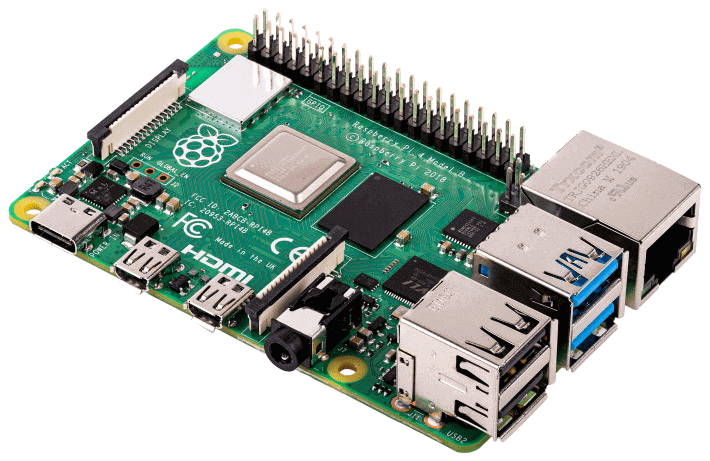
\includegraphics[width=\textwidth]{images/raspberry-pi-4-model-b.png}
    \caption{Raspberry Pi 4 model B. Upraveno z \cite{raspberry-pi-4-model-b}.}
    \label{fig:raspberry-pi-4-model-b}
\end{figure}

\section{Teplotní senzory}
\subsubsection{Teplotní senzory pro krby}
\label{sec:teplotni-senzory-pro-krby}
Pro snímání teploty z kouřovodů u krbů slouží termočlánek typu K od výrobce Guenther. Teplotní rozsah je od -100 °C do 400 °C, takže je dostatečná teplotní rezerva. Průměr kovové ochranné trubičky je 4 mm s délkou 60 mm. Přívodní kabel je dlouhý 3 m se skelným opletením. Termočlánek je zobrazen na obrázku \ref{fig:termoclanek-72-21301041-k}.

\begin{figure}[H]
    \centering
    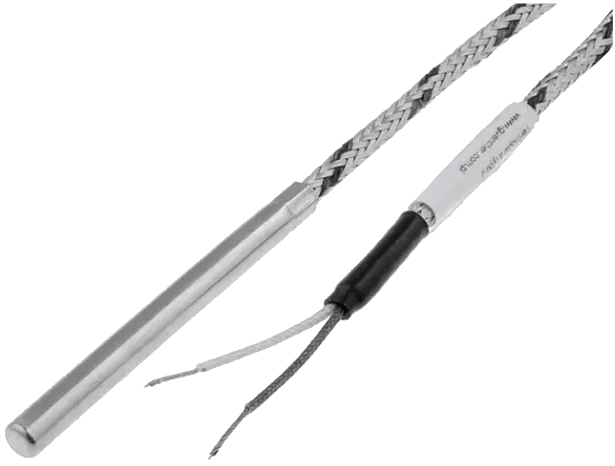
\includegraphics[width=0.5\textwidth]{images/termoclanek-72-21301041-k.png}
    \caption{Termočlánek 72-21301041 typu K \cite{termoclanek-k}.}
    \label{fig:termoclanek-72-21301041-k}
\end{figure}

\subsubsection{Teplotní senzory na 1-Wire sběrnici}
Pro snímání teplot z centrálního zásobníku otopné vody, venkovní teploty a~prostorových teplot z jednotlivých místností slouží teplotní senzor DS18B20 od výrobce Maxim. Umožňuje měřit
v teplotním rozsahu od -+55 °C do +125~°C. V rozsahu od -10 °C do +85 °C měří s přesností ±0,5 °C. Senzor umožňuje měřit teplotu s přesností 12 bitů. Pro komunikaci využívá 1-Wire sběrnici (způsob komunikace je popsán v \ref{sec:1-wire-sbernice} v části 1-Wire sběrnice). Ve svém konkrétním řešením využívám senzory v pouzdře TO-92 pro nástěnné teplotní snímače prostorové teploty, pro centrální zásobník otopné vody a~venkovní teplotu je senzor zapouzdřen do ochranného pouzdra.


\section{\acrshort{dps} se vstupy/výstupu pro Raspberry Pi}
\label{sec:dps-se-vstupy-vystupy-pro-raspberry-pi}

\subsubsection{Datová část 1-Wire sběrnici}
\label{sec:datova-cast-1-wire-sbernice}
Pro zmíněnou 1-Wire sběrnici jsou realizované ESD ochrany spočívající použití Zenerovy diody a  5 $\Omega$ rezistorů, všechny součástky jsou zaintegrované v~jednom pouzdře TSOC, integrovaný obvod je od výrobce Maxim s označením DS9503. Integrovaná Zenerova dioda má nízkou kapacitu desítky pF, tím pádem nepřispívá k nadměrnému kapacitnímu zatěžování sběrnice. Omezovací rezistory slouží k omezení proudu při přepěťovém napěťovém impulzu pro ochranu Zenerovy diody (když je otevřena) před nadměrným proudem během ESD události, při běžné komunikace jsou zanedbatelné. Upínací napětí Zenerovy diody je 5,5 V při 0,9 A (průrazné napětí je přibližně 11 V) během ESD události. Dále je zde zařazena TVS dioda (ESD9L5.0ST5G) s upínacím napětí maximálně 9,8 V při 1 A, slouží jako sekundární ochrana pokud by selhala část s DS9503. 

Další možností je použití galvanického oddělení především pomocí optočlenu. Zde však nastává problém s obousměrnou poloduplexní komunikací, je potřeba zajistit komunikaci oběma směry. Optočleny vkládání zpoždění, které by podle specifikace 1-Wire sběrnice nemělo přesáhnout 1 $\mu$ s. Dále je potřeba oddělený převodník napětí či samotný zdroj pro napájení oddělených částí optočlenu a~další potřebné externí součástky. V neposlední řadě je nutné, alespoň podle výrobce Maxim použít převodník UART na 1-Wire či I$^2$C na 1-Wire sběrnici. Řešení pomocí galvanického oddělení ve výsledku zesložiťuje řešení a též prodražuje. Vzhledem k domácímu nasazení jsem se rozhodl zvolit variantu podle obrázku~\ref{fig:ochrany-1-wire}.

Vzhledem k toleranci napěťové úrovně 3,3 V pro piny u Raspberry Pi, je navržen obousměrný převodník napěťových úrovní z 3,3 V na 5~V a opačně, realizovaný pomocí MOSFET tranzistoru (BSS138P), pull-up rezistorů.

Na obrázku \ref{fig:ochrany-1-wire} jsou vidět dvě větve pro 1-Wire sběrnici, je to z důvodu dvou typů zařízení, teplotních čidel DS18B20 a  zesilovače s termočlánkem, které mají různé časování, popsáno více níže. Sběrnici, lze sdružit do jedné pomocí propojky P6.

\begin{figure}[H]
    \centering
    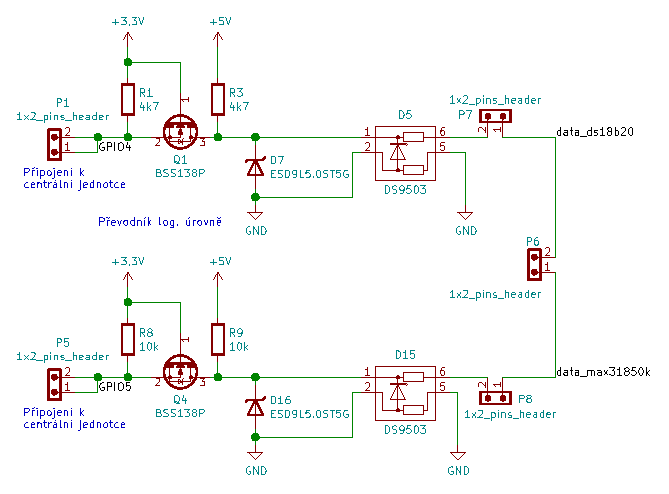
\includegraphics[width=\textwidth]{images/svg/kicad/ochrany-1-wire.eps}
    \caption[ESD ochrany pro 1-Wire sběrnici s převodním napěťových úrovní]{ESD ochrany pro 1-Wire sběrnici s převodním napěťových úrovní. Kolíková lišta P1, P5 je připojena na Raspberry Pi.}
    \label{fig:ochrany-1-wire}
\end{figure}


\subsubsection{Napájení 1-Wire sběrnice}
\label{sec:napajeni-1-wire-sbernice}
Pro ochranu napájení 1-Wire sběrnice (5 V) jsou veškerá koncové teplotní senzory napájené přes elektronickou pojistku od Texas Instrumenst s označením TPS2600, obrázek \ref{fig:ochrana-napajeni-1-wire}. Která zajišťuje ochranu pro vstupní napětí, hlídá maximální hodnotu vstupního napětí do nastavené meze 5,25 V (maximální hranice je 60 V), minimální vstupní napětí do nastavené meze 4,75 V (minimální hranice je -60 V). Vstupní omezení napětí je pomocí rezistorů R5, R10, R11 a R12. Omezovací proud je nastaven na přibližně 73 mA (hodnotu lze změnit přes potenciometr R17), při jeho překročení dojde k odpojení výstupu pod dobu dokud nedojde k odstranění závady. Kondenzátor C2 nastavuje rychlost náběhu výstupního napětí. Pro indikaci chyb napájení je zde červená LED.

\begin{figure}[H]
    \centering
    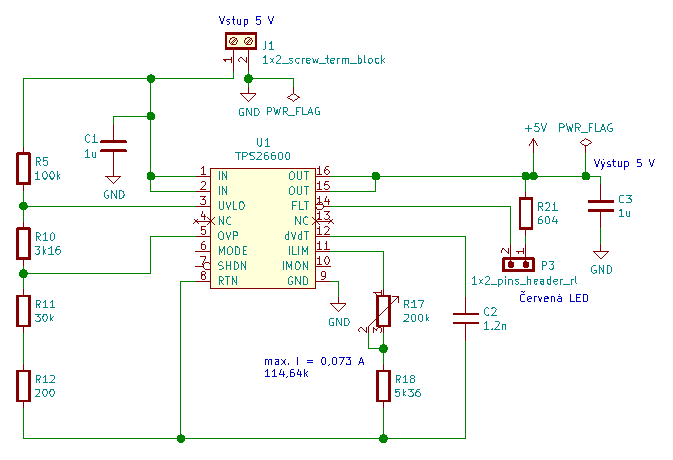
\includegraphics[width=\textwidth]{images/svg/kicad/ochrana-napajeni-1-wire.eps}
    \caption[Obvod TPS26600 pro ochranu napájení 1-Wire sběrnice.]{Obvod TPS26600 pro ochranu napájení 1-Wire sběrnice.}
    \label{fig:ochrana-napajeni-1-wire}
\end{figure}

\subsubsection{Ochrana pro chodbové nástěnné termostaty}
Obdobně jako v části \ref{sec:datova-cast-1-wire-sbernice} (Datová část 1-Wire sběrnice) je stejná ochrana pro snímání logické úrovně z~chodbových nástěnných termostatů. Při sepnutí chodbového termostatu na daném patře je detekována log. 0 (požadavek na vytápění) v opačném případě je zde log. 1 (zastavení vytápění). Chodbové nástěnné termostaty jsou popsány v sekci \ref{digitalni-chodbove-termostaty}.

\subsubsection{Ochrana napájení 3,3 V}
Přímo z Raspberry Pi je využito napětí 3,3 V pro převodník napětí, popsaný v~části \ref{sec:datova-cast-1-wire-sbernice} (datová část 1-Wire sběrnice). Zde je použita vratná pojistka polymerový PTC (RXEF005) se spínacím proudem 100 mA, pro omezení proudu v~případě poruchy, dále je zde transilová dioda (SM2T3V3A) pro ochranu při přepětí (s~upínacím napětí max. 6,5 V (při 25 A, 10/1000~µs), průrazné napětí 3,6 V). Na obrázku \ref{fig:ochrana-napajeni-3_3-v} je zobrazena popsaná ochrana.

\begin{figure}[H]
    \centering
    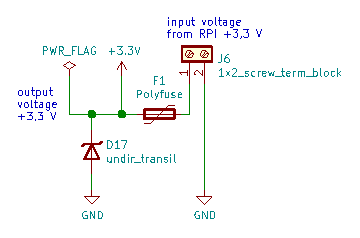
\includegraphics[width=0.6\textwidth]{images/svg/kicad/ochrana-napajeni-3_3-v.eps}
    \caption[Ochrana pro napájení 3,3 V z Raspberry Pi.]{Ochrana pro napájení 3,3 V z Raspberry Pi.}
    \label{fig:ochrana-napajeni-3_3-v}
\end{figure}

\subsubsection{Způsob realizace 1-Wire sběrnice}
Samotná 1-Wire sběrnice je realizovaná pomocí UTP kabelu kategorie Cat5e. Na pinu číslo 4 jsou DATA, na pinu 5 je zem (GND) a na pinu 3 je napájení 5~V. Ze samotné DPS je sběrnice vyvedena pomocí konektorů RJ45, čtyři konektory pro teplotní senzory DS18B20 a čtyři pro termočlánky s MAX31850K.

\subsubsection{Realizovaná DPS ochran pro centrální jednotku Raspberry Pi}
Na obrázku \ref{fig:dps-rpi-1-wire-termostaty-ochrany-spodek} a \ref{fig:dps-rpi-1-wire-termostaty-ochrany-vrsek} je realizovaná DPS vstupů/výstupů pro centrální jednotku Raspberry Pi. Deska byla vlastnoručně navržena, vyrobena a osazena. Je aplikován ochranný lak, na vrchní propojky byl též aplikován ochranný lak a následně zakryty tavnou plastovou hmotou.

\begin{figure}[H]
    \centering
    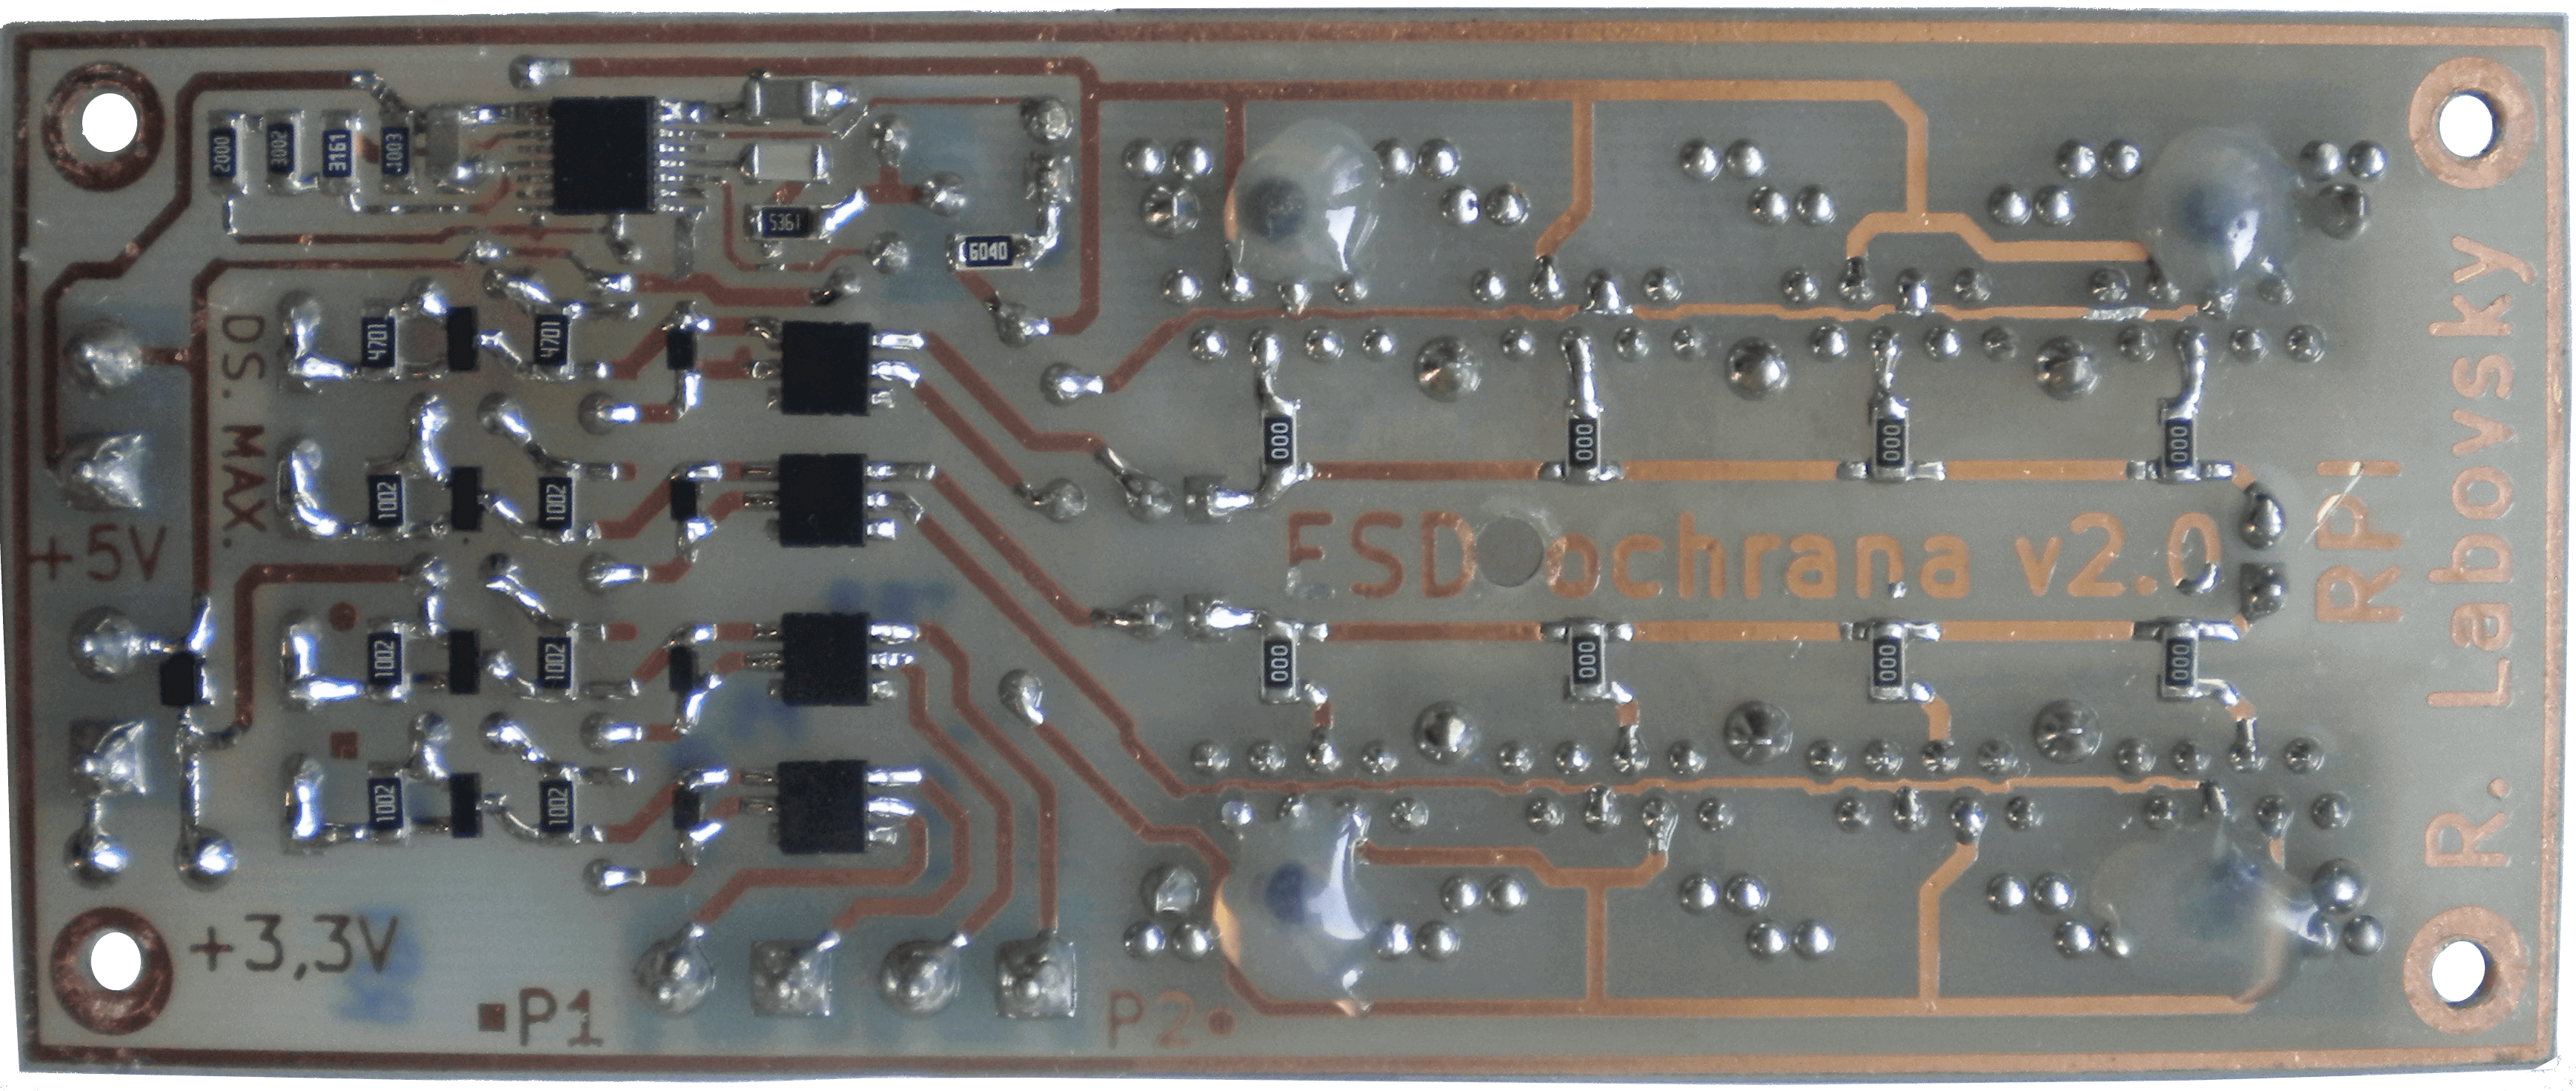
\includegraphics[width=\textwidth]{images/dps-rpi-1-wire-termostaty-ochrany-spodek.png}
    \caption[Spodní část DPS pro ochranu vstupů/výstupů pro centrální jednotku Raspberry Pi.]{Spodní část DPS pro ochranu vstupů/výstupů pro centrální jednotku Raspberry Pi.}
    \label{fig:dps-rpi-1-wire-termostaty-ochrany-spodek}
\end{figure}

\begin{figure}[H]
    \centering
    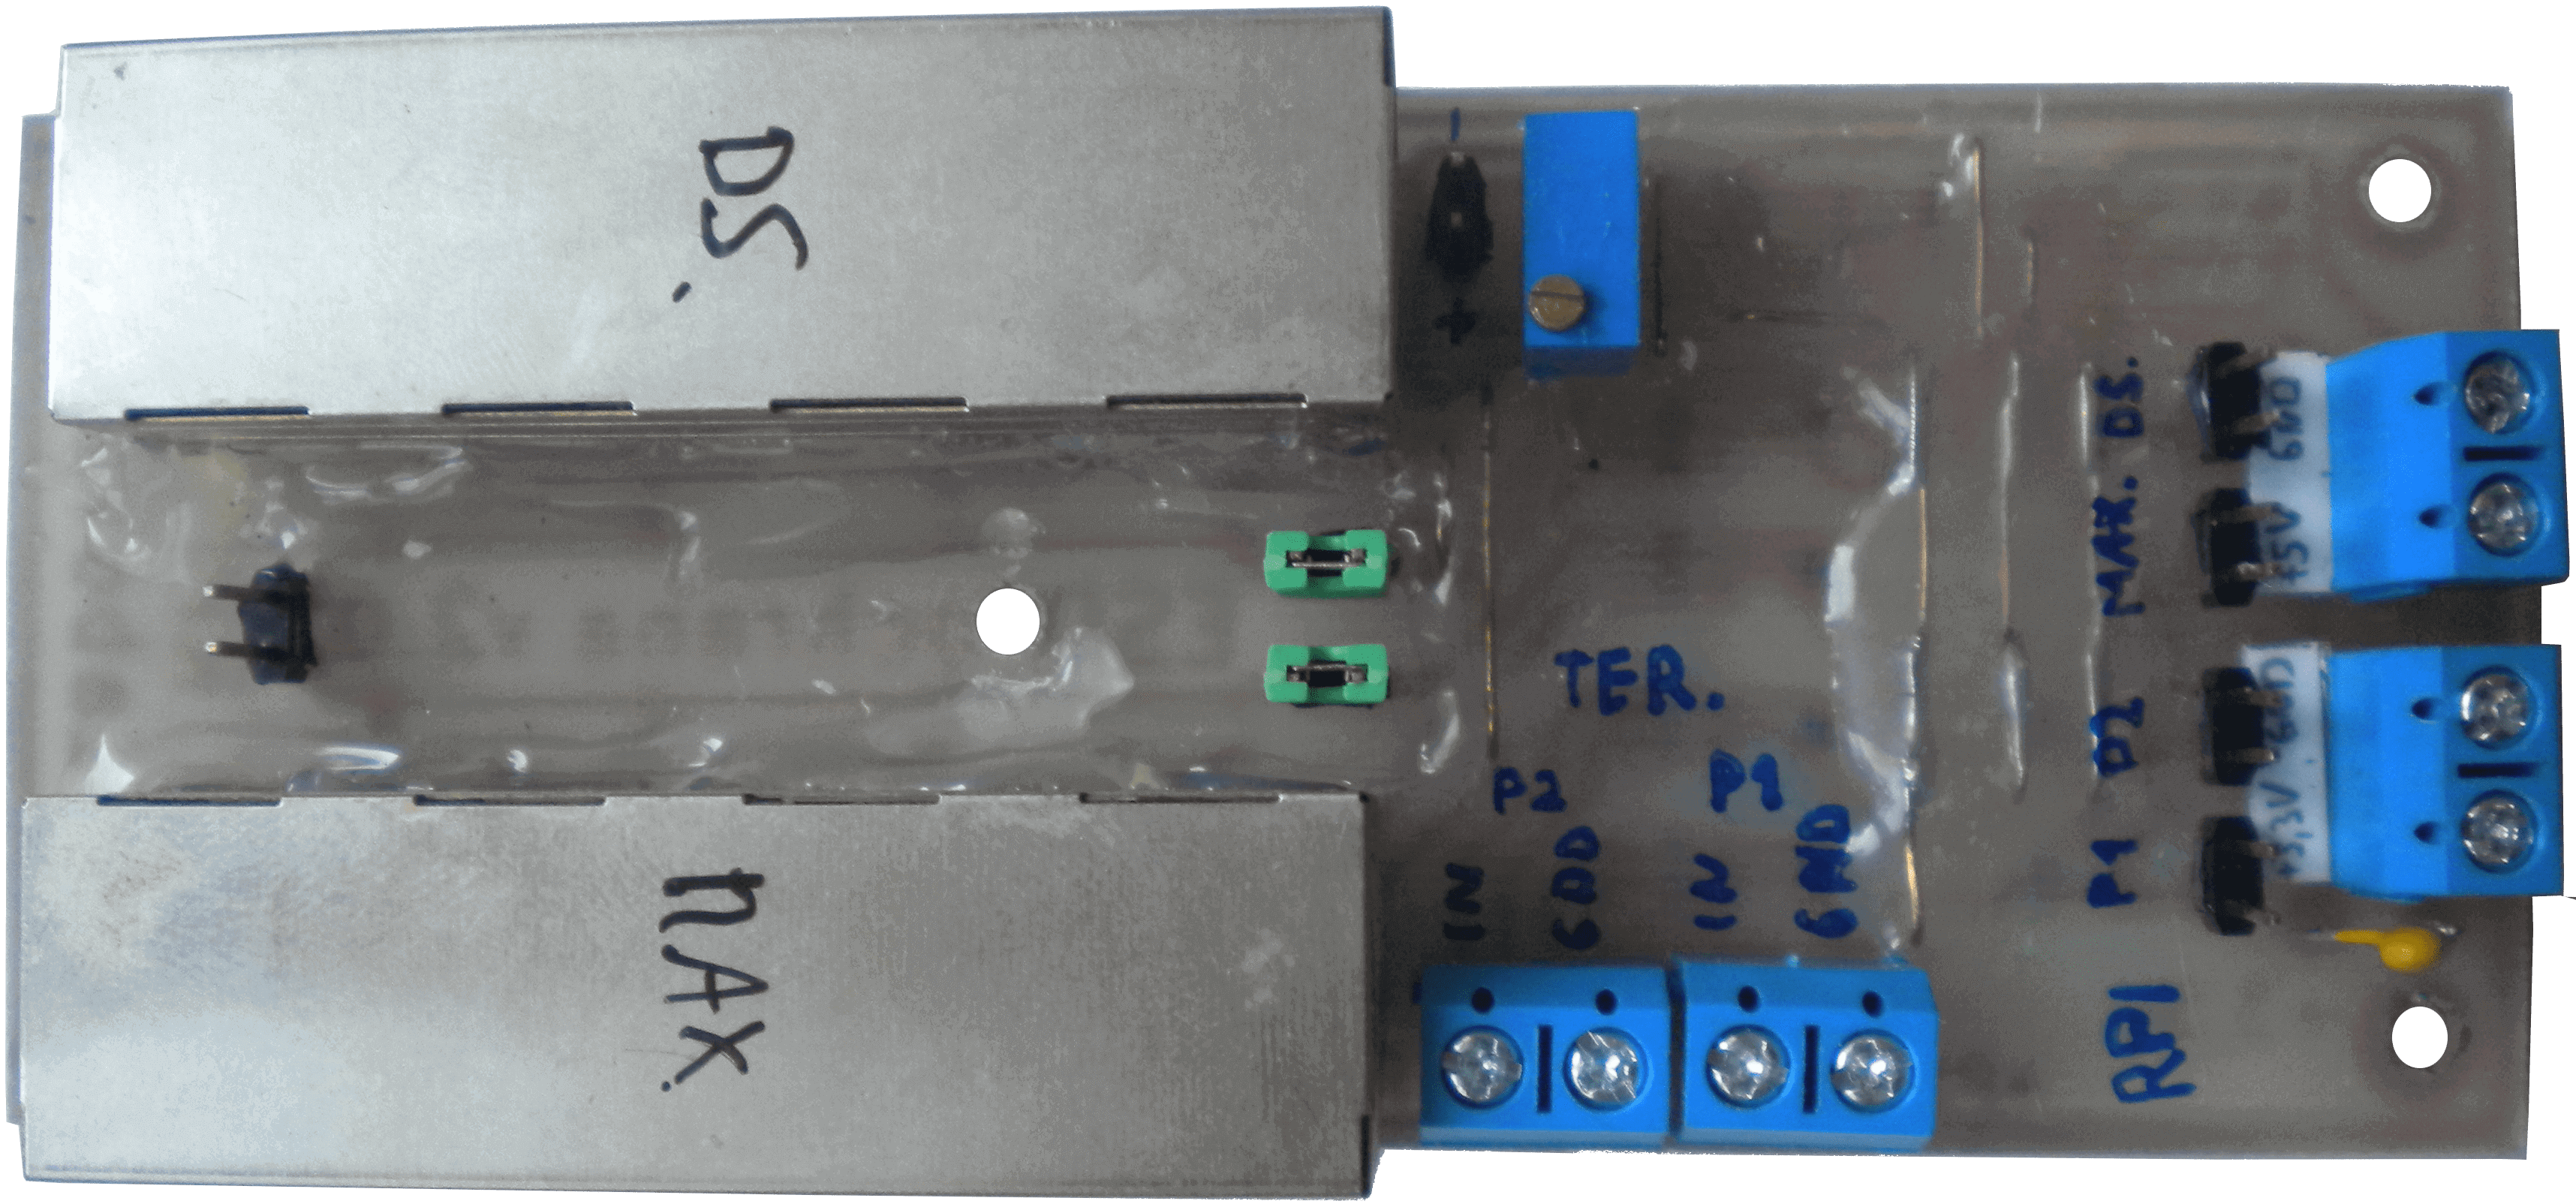
\includegraphics[width=\textwidth]{images/dps-rpi-1-wire-termostaty-ochrany-vrsek.png}
    \caption[Vrchní část DPS pro ochranu vstupů/výstupů pro Raspberry Pi.]{Vrchní část DPS pro ochranu vstupů/výstupů pro Raspberry Pi.}
    \label{fig:dps-rpi-1-wire-termostaty-ochrany-vrsek}
\end{figure}

\section{DPS u krbů}
Navržená DPS se skládá z části elektronické pojistky TPS2600, zapojení je obdobné jako v \ref{sec:napajeni-1-wire-sbernice} (napájení 1-Wire sběrnice), navíc je na vstupu připojena transilová dioda (ESD9L5.0ST5G). Napěťové meze jsou nastaveny stejně, tedy minimální napětí je 4,75 V, maximální 5,25 V, proud je omezen na maximální hodnotu 100 mA. Dále je zde přivedena 1-Wire sběrnice přes konektor RJ45 s~obdobnými ochranami jako v \ref{sec:datova-cast-1-wire-sbernice} (datová část 1-Wire sběrnice), včetně stejných ochran pro napájení, pro připojení MAX31850K přes svorkovnici. V neposlední řadě jsou zde vstupy pro ovládání třech LED pro signalizaci (obrázek \ref{fig:ochrana-krby-lcd-teplotni-senzor}) naakumulovaného zásobníku otopné vody, modrá led signalizuje stav horní části zásobníku, oranžová LED je pro střední část, červená je pro signalizaci spodní části. Vstupní část je chráněná přes DS9503 a transilovou diodou (ESD9L5.0ST5G). Sepnutí LED je přes tranzistor (BSS138P). Obdobně jsou řešeny oranžová a modrá LED.

\begin{figure}[H]
    \centering
    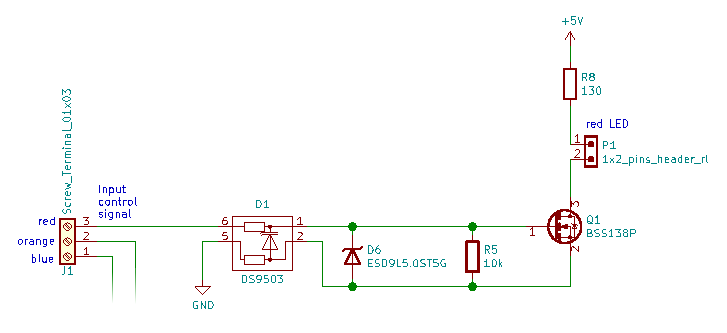
\includegraphics[width=\textwidth]{images/svg/kicad/ochrana-krby-lcd-teplotni-senzor.eps}
    \caption[Zapojení pro ovládání signalizační červené LED.]{Zapojení pro ovládání signalizační červené LED.}
    \label{fig:ochrana-krby-lcd-teplotni-senzor}
\end{figure}

\subsubsection{I$^2$C sběrnice}
\label{ses:i2c-sbernice}
Sběrnice I$^2$C je realizovaná pomocí zakoupeného modulu (obrázek \ref{fig:modul-pca9615-i2c-sbernice}) s~obvodem PCA9615 do firmy  NXP Semiconductors. Vstupní signál SCL a~SDA je veden přímo z~centrální jednotky na vstupu obovodu PCA9615, napájení je s 3,3 V logikou. Výstup z PCA9615 je pomocí diferenciální vedení, pro každý signál SCL a~SDA jsou použity dva vodiče. Napájení na této straně je pomocí 5 V. Sběrnice je realizovaná pomocí UTP Cat5e, výstup z~modulu je realizován pomocí konektoru RJ45. Vzhledem k použití UTP kabelu a diferenciálnímu přenosu je možné dosáhnout velké vzdálenosti sběrnice. Nejdelší bod dosahuje přibližně 30 m, je tedy možné použít I$^2$C sběrnici na vzdálenost pro kterou není standartě dělána. Použitá frekvence je 100~kHz. Jedná se tedy o plnohodnotnou I$^2$C sběrnici. Důvodem pro zvolení této varianty bylo na základě výběru displeje s I$^2$C sběrnicí (jednoduché a~levné řešení), dále jedná se o klasické zapojení displeje jako by se nalézal v~krátké vzdálenosti od centrální jednotky a není tak nutný převod jako při využít např. RS485 na UART a následně na I$^2$C sběrnici, v neposlední řadě komunikace je definována podle protokolu I$^2$C.  Jeden modul se nalézá na straně centrální jednotky a pak na straně krbů. Napájení 5 V je realizováno pomocí samostatných kabelů, není tedy součástí UTP kabelu. Z důvodu omezení kabeláže je sběrnice realizována v jednom UTP kabelu s 1-Wire sběrnicí, tedy přesněji jsou využity volné vodiče s číslem 1,2 pro SCL a 7,~8 pro SDA. Zařízení lze zapojovat jak na straně před PCA9615, tak i~na diferenciální straně, je však výhodné připojené uzly udržet co v nejkratší vzdálenosti kvůli degradování výkonu. Blokové schéma je na obrázku \ref{fig:blokove-schema-pca9615-i2c-sbernice} včetně napojení uzlů. Schéma zapojení modulu je na obrázku \ref{fig:zapojeni-pca9615-i2c-sbernice}.

\begin{figure}[H]
    \centering
    \def\svgwidth{\columnwidth}
    \input{images/svg/blokove-schema-pca9615-i2c-sbernice.pdf_tex}
    \caption{Blokové schéma zapojení obvodu PCA9615 s impedančním zakončením sběrnice a možnostmi napojení uzlů. Upraveno z \cite{pca9615-schema-zapojeni}.}
    \label{fig:blokove-schema-pca9615-i2c-sbernice}
\end{figure}

\begin{figure}[H]
    \centering
    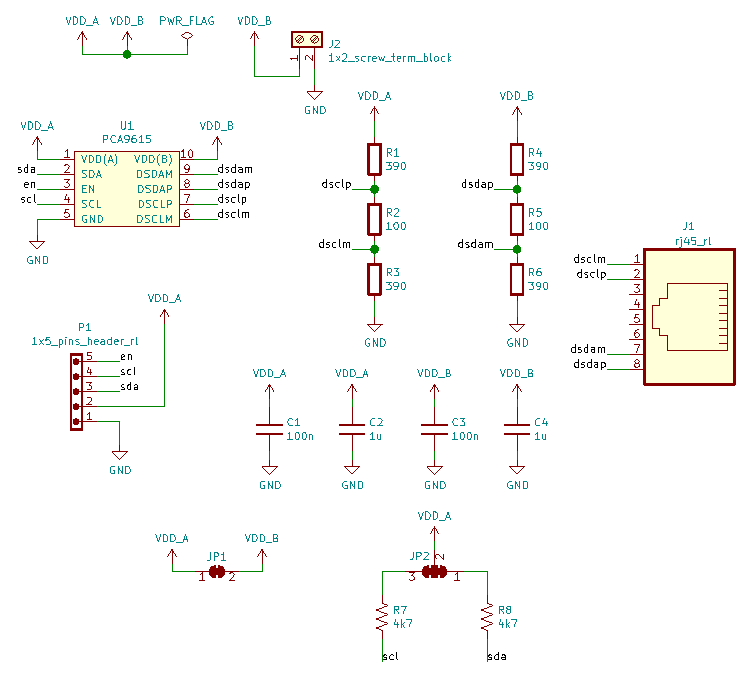
\includegraphics[width=\textwidth]{images/svg/kicad/zapojeni-pca9615-i2c-sbernice.eps}
    \caption{Zapojení PCA9615 v modulu. Upraveno z \cite{pca9615-schema-zapojeni}.}
    \label{fig:zapojeni-pca9615-i2c-sbernice}
\end{figure}

Výhodou PCA9615 je automatický výběr směru komunikace, není potřeba externího ovládání. Komunikace je možná až do rychlosti 1 MHz (přibližně pro 3 m), se zvýšenou délkou je však nutné rychlost snížit. Komunikace využívá standardního protokolu I$^2$C. ESD ochrana, v případě naindukování přepětí po cestě. Nezávislost napájení, je možné napájet koncová zařízení z jiného zdroje než Master. V neposlední řadě se jedná o jednoduché řešení bez nutných další zařízení na straně Slave, stačí pouze zapojit koncové zařízení s podporou I$^2$C.

\begin{figure}[H]
    \centering
    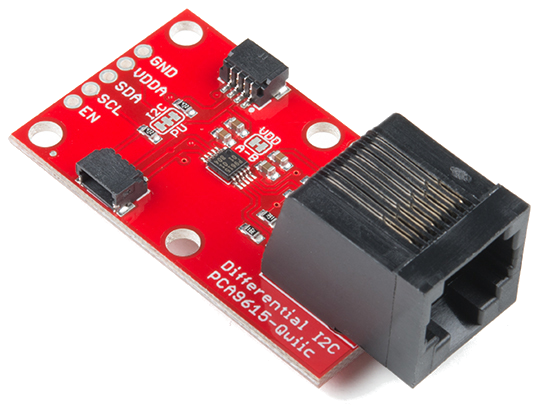
\includegraphics[width=0.6\textwidth]{images/modul-pca9615-i2c-sbernice.png}
    \caption[Modul s obvodem PCA9615.]{Modul s obvodem PCA9615 \cite{pca9615-i2c-modul}.}
    \label{fig:modul-pca9615-i2c-sbernice}
\end{figure}

\subsubsection{Měření teploty pomocí termočlánku a převodníku MAX31850K}
Teplotní senzory připojené na kouřovody krbů jsou realizované pomocí termočlánku z \ref{sec:teplotni-senzory-pro-krby}. Termočlánky jsou připojené k zakoupenému modulu (obrázek~\ref{fig:modul-max31850k-1-wire-prevodnik-termoclanku}) se zesilovačem napětí generované termočlánkem, hodnota napětí je následně převedena do digitální podoby včetně teplotní kompenzace studeného konce termočlánku a~tato hodnota je posílaná po 1-Wire sběrnici. Je možné připojit termočlánky typu K, J, N, S, R nebo E. Převodník umožňuje měřit teplotu s převodem pomocí AD převodníku až na 14 bitů. Rozlišení teploty činí 0,25 °C. Při teplotách -200 °C až 700 °C činí přesnost měřené teploty ±2~°C. Obvod disponuje detekcí zkratu (na GND nebo napájení) na vstupu pro termočlánek. Dále je zde detekci odpojeného termočlánku. Schéma zapojení modulu je na obrázku \ref{fig:zapojeni-max31850k-1-wire-prevodnik-termoclanku}.

\begin{figure}[H]
    \centering
    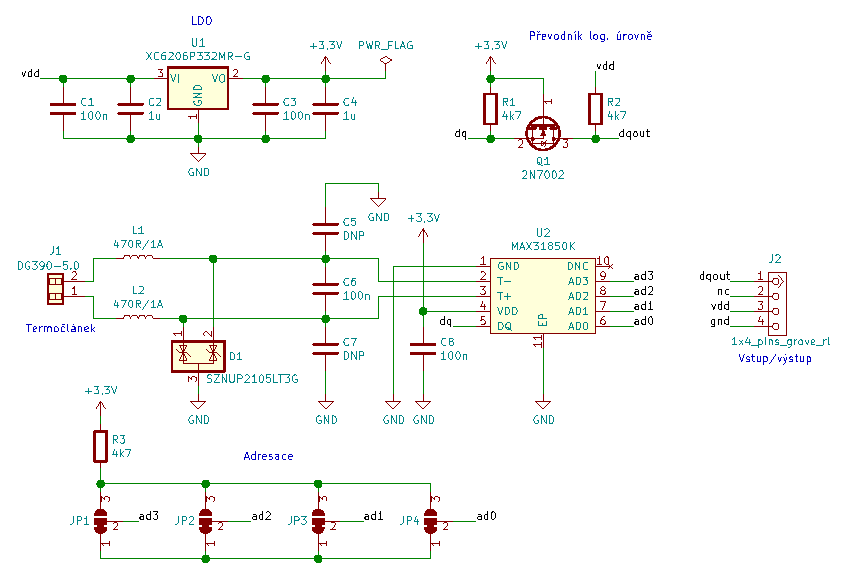
\includegraphics[width=\textwidth]{images/svg/kicad/zapojeni-max31850k-1-wire-prevodnik-termoclanku.eps}
    \caption[Zapojení MAX31850K v modulu.]{Zapojení MAX31850K v modulu. Upraveno z \cite{prevodnik-max31850k}.}
    \label{fig:zapojeni-max31850k-1-wire-prevodnik-termoclanku}
\end{figure}

\begin{figure}[H]
    \centering
    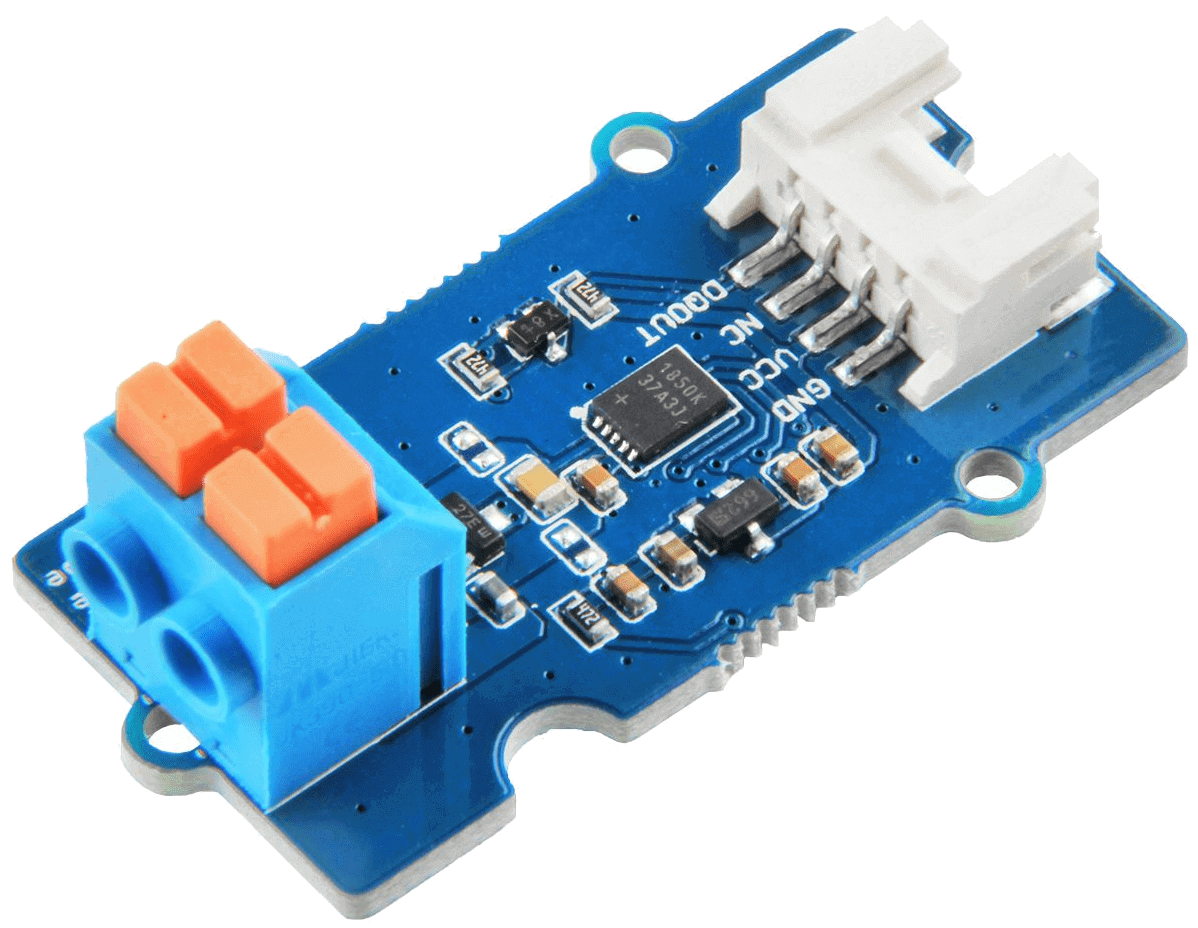
\includegraphics[width=0.6\textwidth]{images/modul-max31850k-1-wire-prevodnik-termoclanku.png}
    \caption[Modul s obvodem MAX31850K.]{Modul s obvodem MAX31850K \cite{prevodnik-max31850k}.}
    \label{fig:modul-max31850k-1-wire-prevodnik-termoclanku}
\end{figure}

\subsubsection{Realizace 1-Wire sběrnice u zásobníku otopné vody}
Na obrázku \ref{fig:dps-1-wire-sbernice-u-zasobniku-otopne-vody} je realizovaná DPS pro teplotní senzory u zásobníku otopné vody. Princip zapojení včetně ochrana na napájecí i datové části je popsán v části \ref{sec:dps-se-vstupy-vystupy-pro-raspberry-pi} (datová část 1-Wire sběrnice). Na obrázku \ref{fig:instalacni-krabice-cidla-u-zasobniku-otopne-vody} je vidět horní část DPS vložená do instalační krabice. Celkově je zde k dispozici 6 pozic pro upevnění přes svorkovnice teplotní senzory. V současnosti jsou zde napojeny pouze 3 teplotní senzory (pro snímání teplot z horní, střední a spodní části zásobníku otopné vody). Na obrázku \ref{fig:ds18b20-ochrana} je teplotní senzor DS18B20 v pouzdře TO-92 připevněn na UTP kabel a zataven plastovou hmotou na níž je následně nanesena smršťovací ochranná bužírka. Na obrázku \ref{fig:zasobnik-otopné-vody} jsou vyznačená místa s umístěním teplotních senzorů.

\begin{figure}[H]
    \centering
    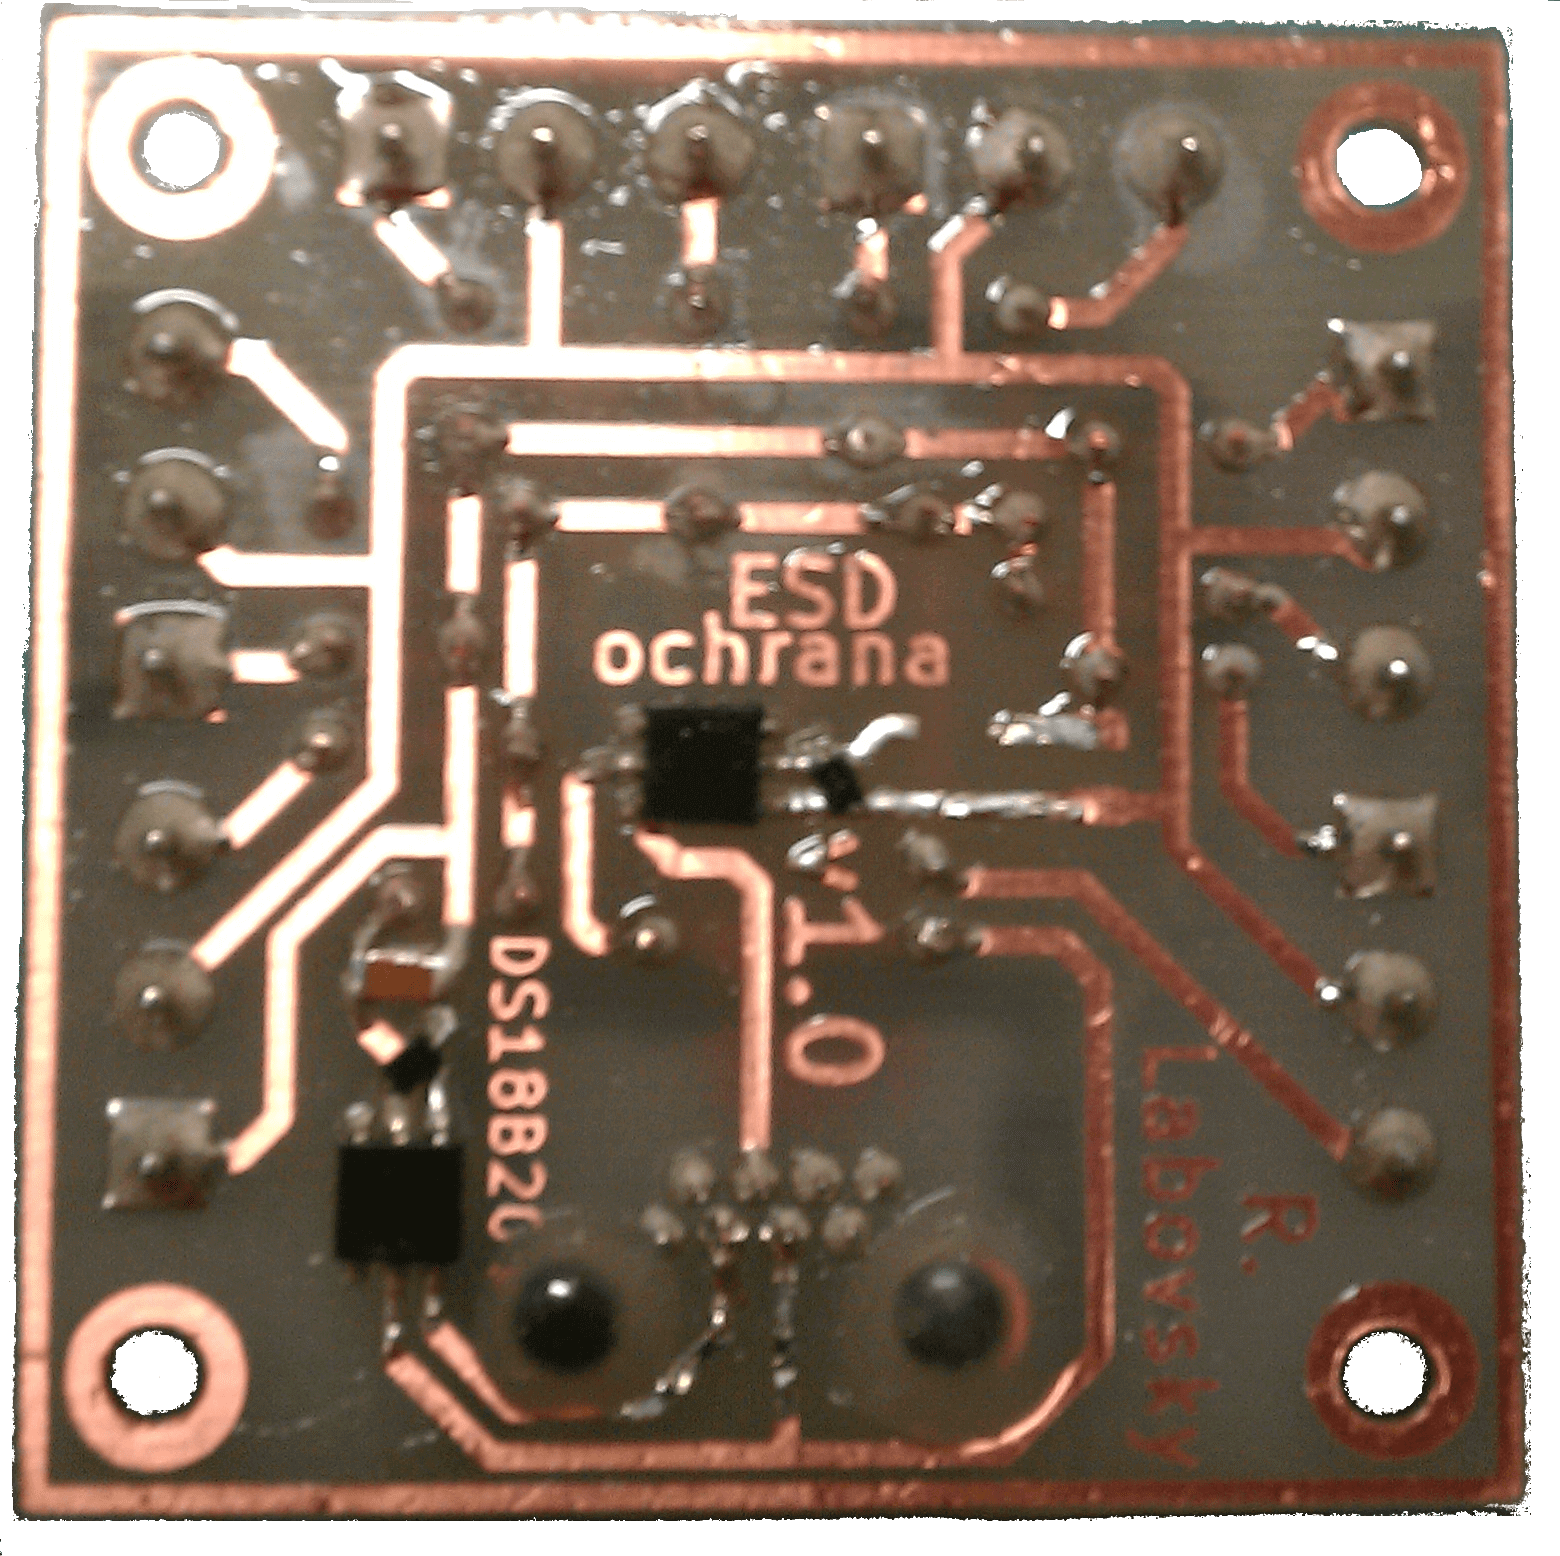
\includegraphics[width=0.6\textwidth]{images/dps-1-wire-sbernice-u-zasobniku-otopne-vody.png}
    \caption{Realizovaná DPS pro teplotní senzory 1-Wire sběrnice u zásobníku otopné vody.}
    \label{fig:dps-1-wire-sbernice-u-zasobniku-otopne-vody}
\end{figure}

\begin{figure}[H]
    \centering
    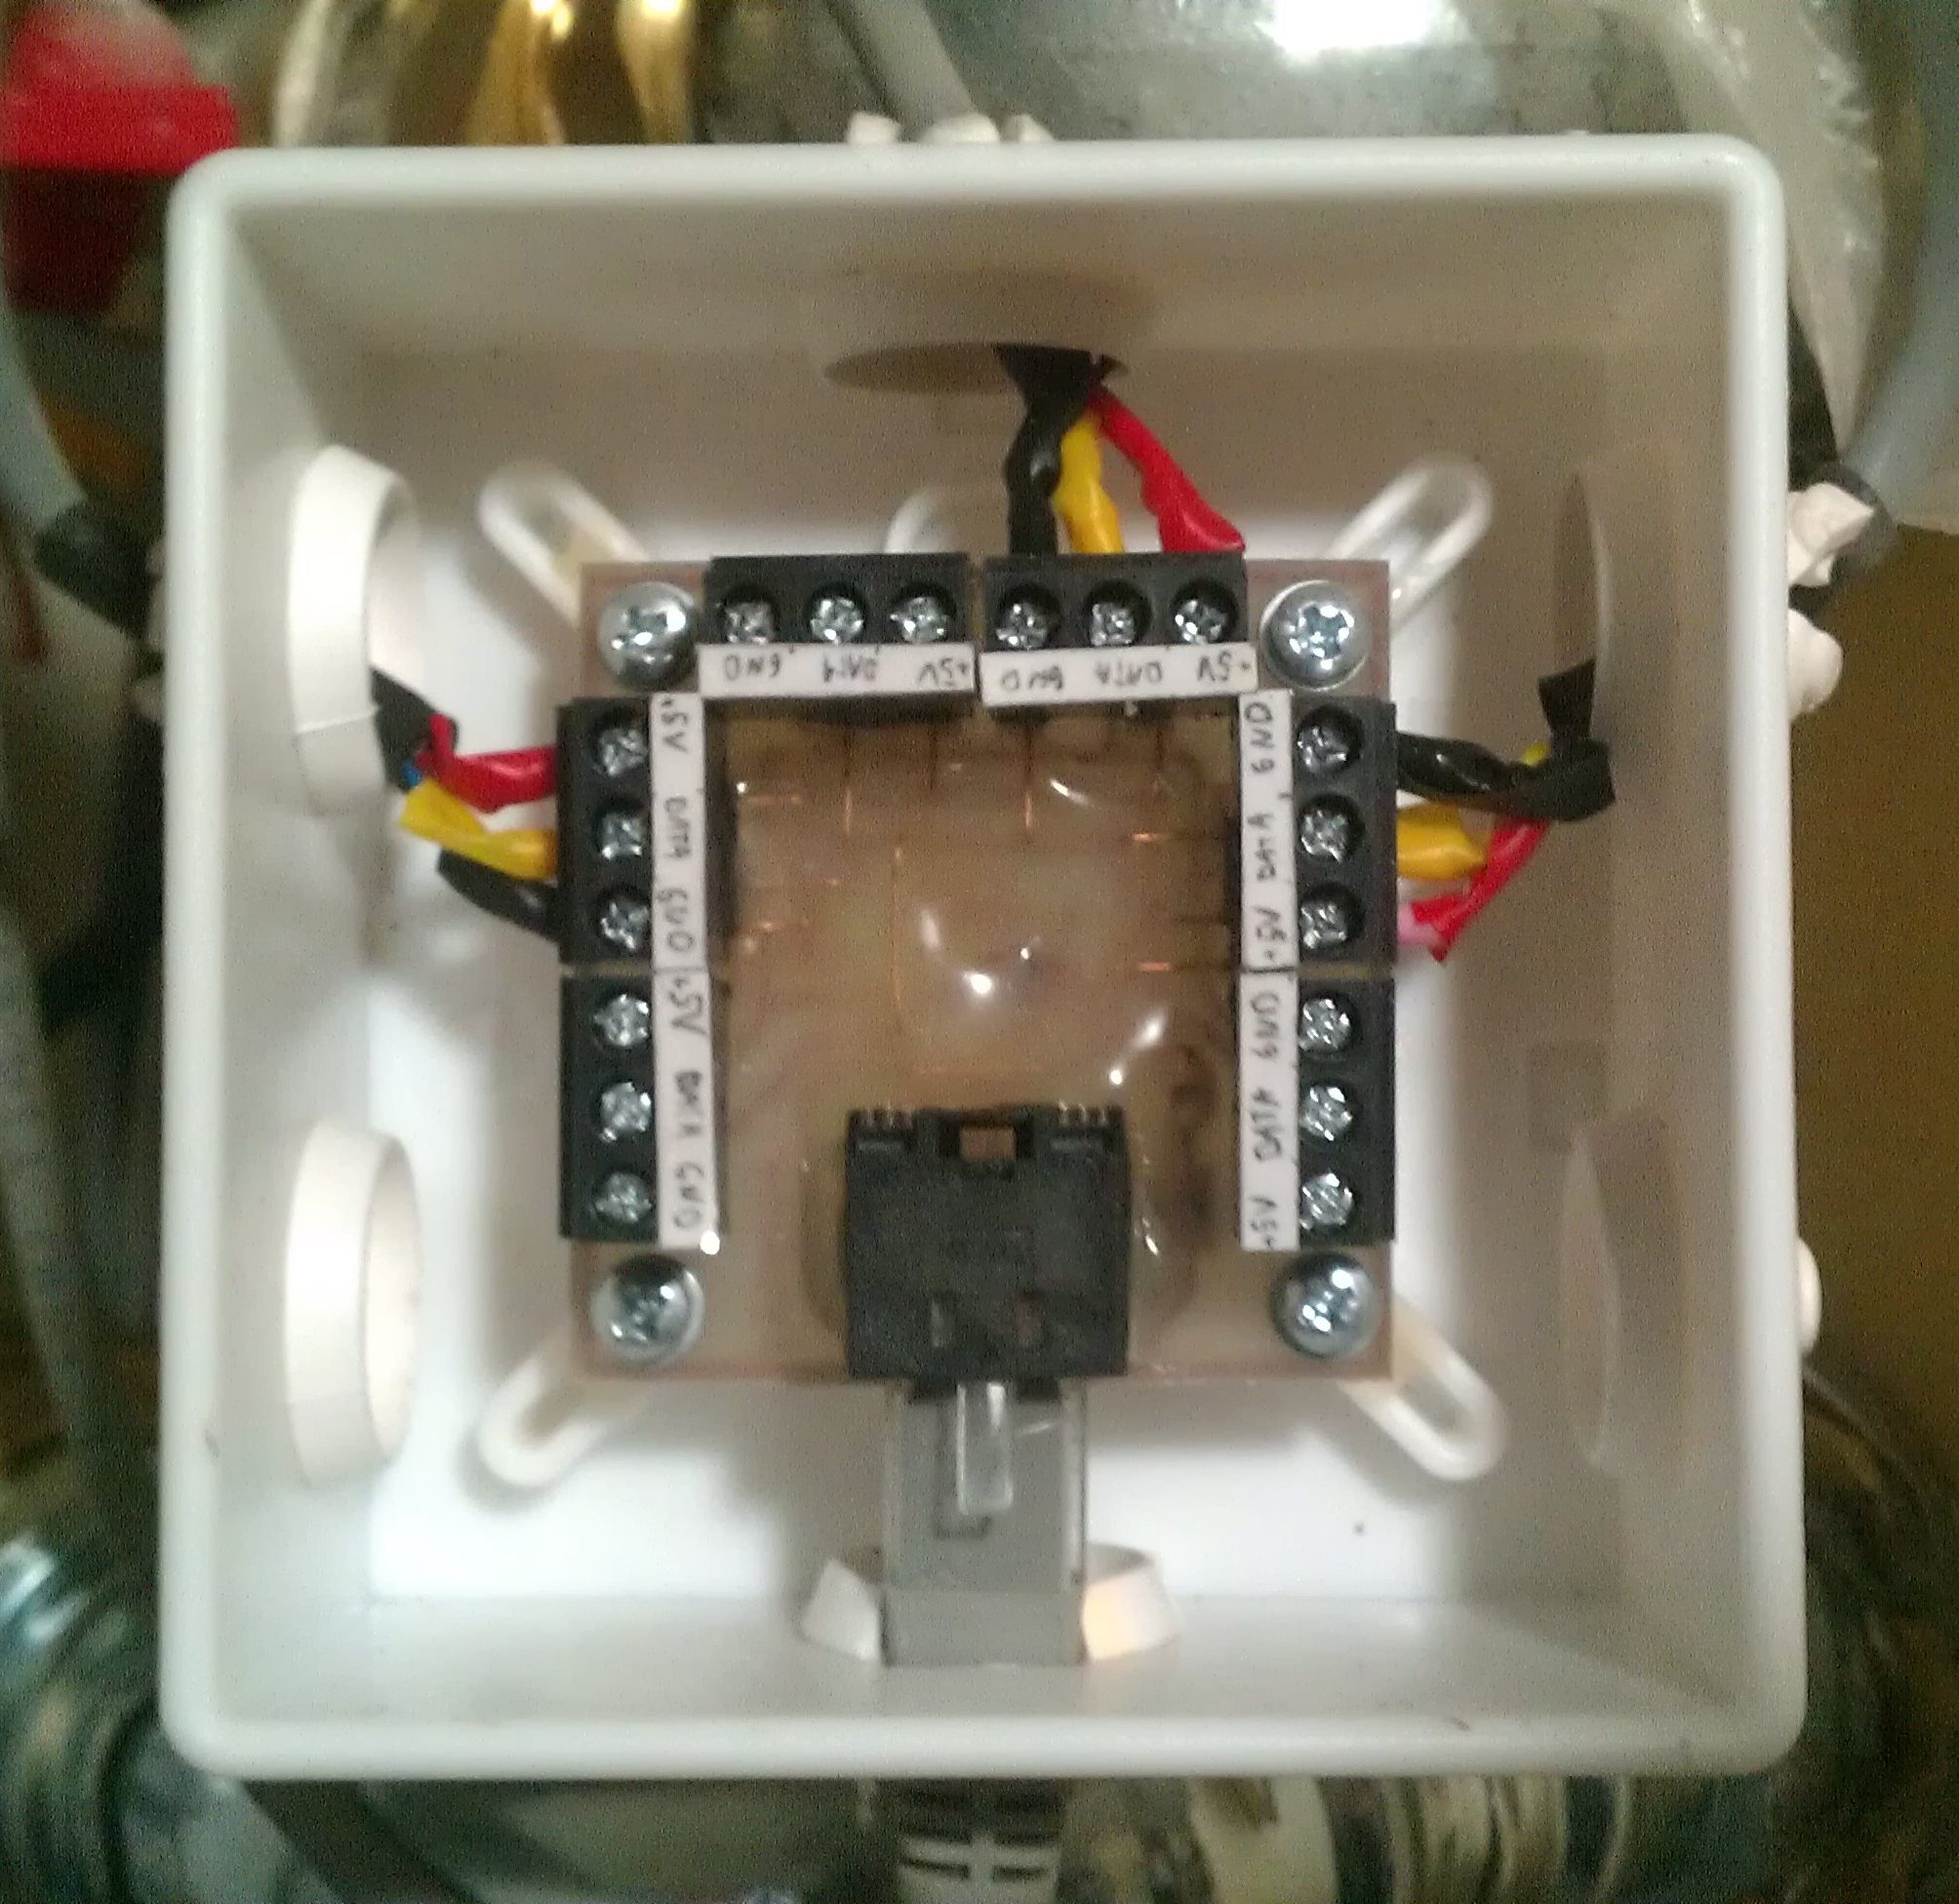
\includegraphics[width=0.6\textwidth]{images/instalacni-krabice-cidla-u-zasobniku-otopne-vody.png}
    \caption{Horní části DPS vložená do instalační krabice.}
    \label{fig:instalacni-krabice-cidla-u-zasobniku-otopne-vody}
\end{figure}

\begin{figure}[H]
    \centering
    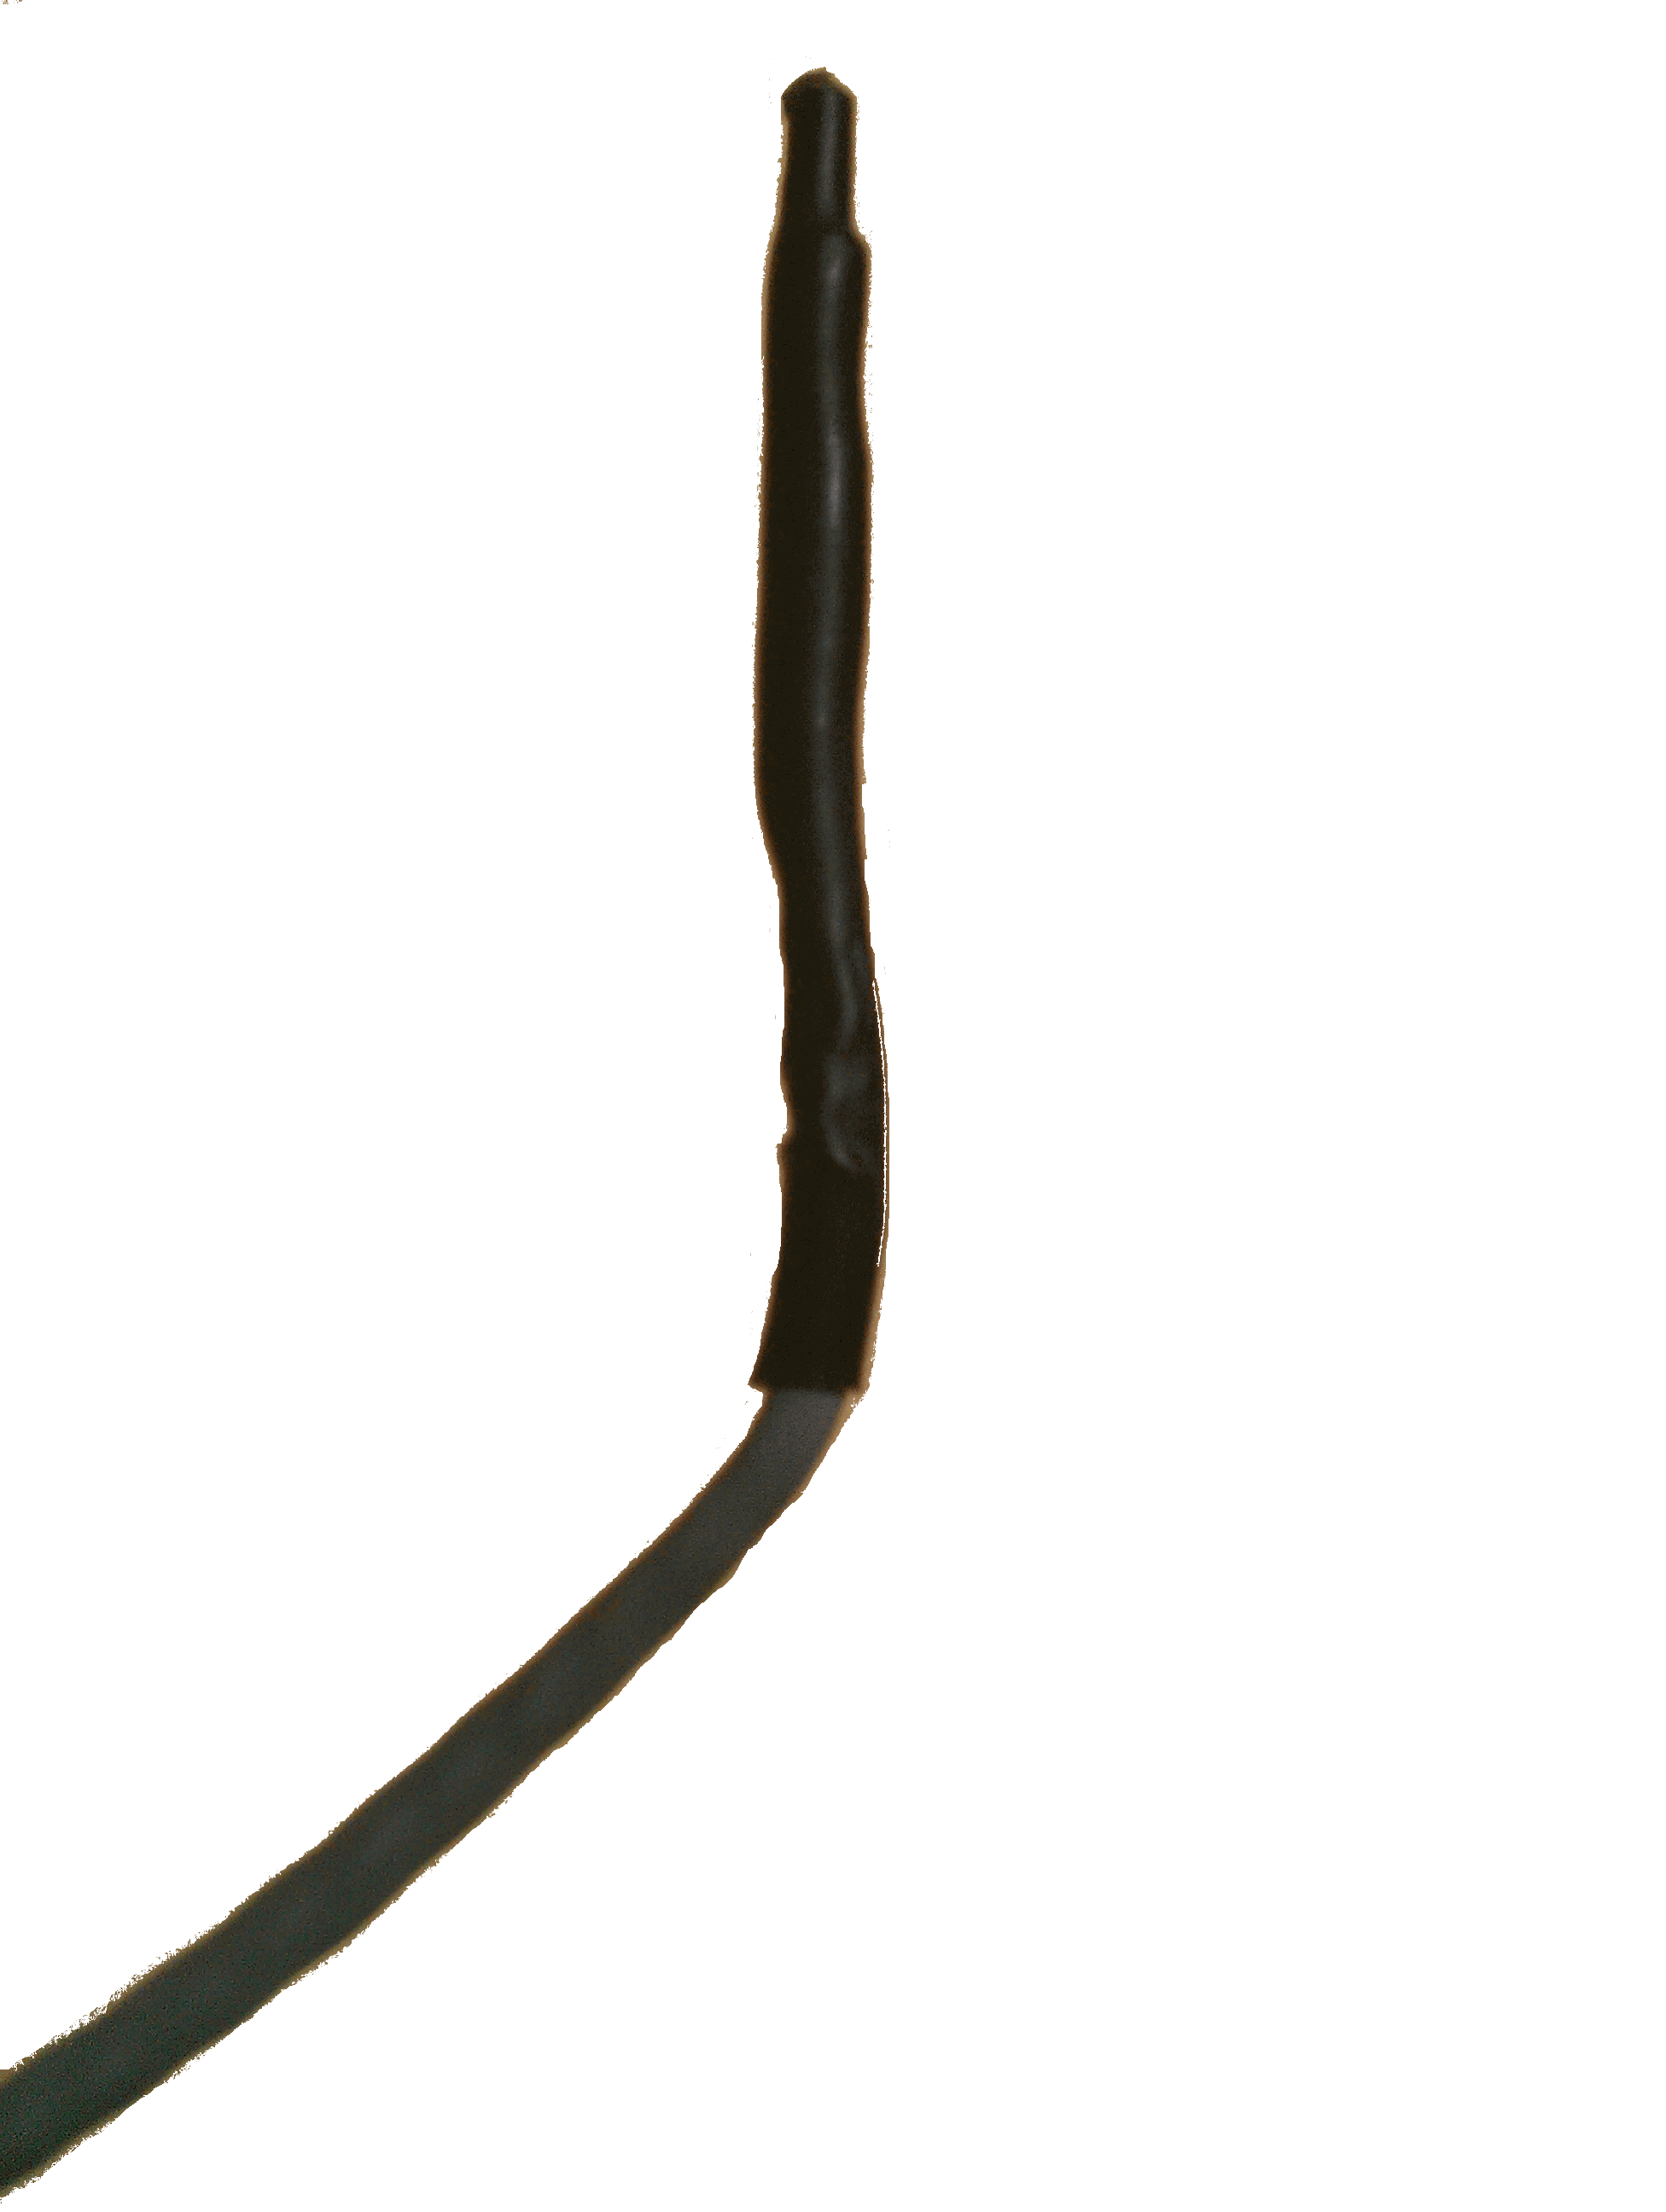
\includegraphics[width=0.6\textwidth]{images/ds18b20-ochrana.png}
    \caption{Teplotní senzor DS18B20 v ochranném pouzdře.}
    \label{fig:ds18b20-ochrana}
\end{figure}

\begin{figure}[H]
    \centering
    \includegraphics[width=\textwidth]{images/zasobnik-otopné-vody.png}
    \caption[Zásobník otopné vody.]{Zásobník otopné vody. Červené kroužky označují místa teplotních senzorů.}
    \label{fig:zasobnik-otopné-vody}
\end{figure}


\subsubsection{LCD displej}
Pro zobrazování teplot ze střední a spodní části zásobníku otopné vody byl zvolen 16 znakový a 2 řádkový LCD displej s modrým podsvícením a~bílými písmeny (obrázek ). Po obsluhu displeje slouží řadič HD44780. K~řadiči je připojen I$^2$C expandér PCF8574 s osmi výstupy, které jsou připojená na datovou sběrnici pro ovládání respektive zobrazování znaků na displeji. Displej je zapojen za modulem popsaným v části \ref{ses:i2c-sbernice} (I$^2$C). Každý displej, respektive expandér PCF8574 umožňuje nastavit pomocí propojek A0, A1, A2 unikátní adresu zařízení na sběrnici.

\begin{figure}[H]
\centering
\begin{subfigure}{.5\textwidth}
  \centering
  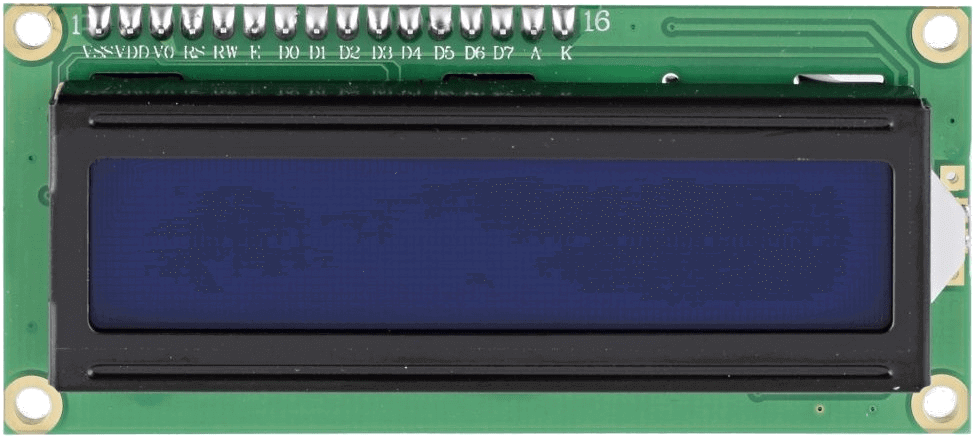
\includegraphics[width=0.9\linewidth]{images/predni-cast-lcd-displeje.png}
  \caption{Přední část displeje.}
  \label{fig:predni-cast-lcd-displeje}
\end{subfigure}%
\begin{subfigure}{.5\textwidth}
  \centering
  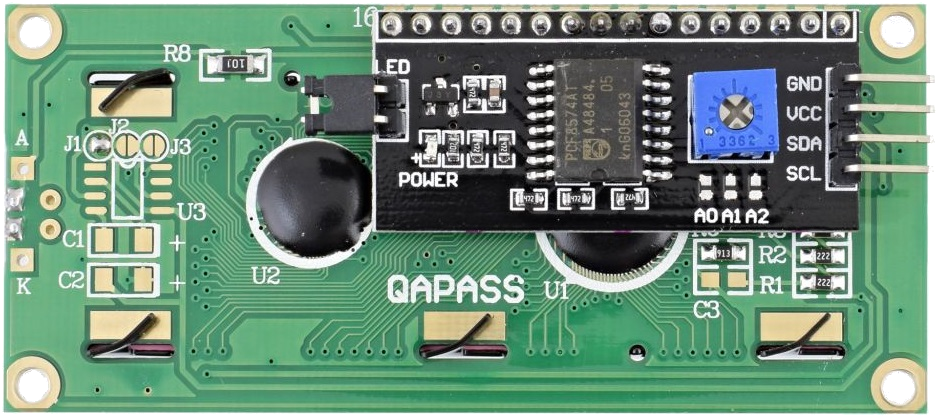
\includegraphics[width=0.9\linewidth]{images/zadni-cast-lcd-displeje-s-expanderem-pcf8574.png}
  \caption{Zadní část displeje s I$^2$C expandérem PCF8574.}
  \label{fig:zadni-cast-lcd-displeje-s-expanderem-pcf857}
\end{subfigure}
\caption{LCD displej pro zobrazování teplot ze zásobníku otopné vody \cite{lcd-displej}.}
\label{fig:lcd-displej}
\end{figure}

\subsubsection{Realizovaná DPS ochran a signalizace u krbů}

\begin{figure}[H]
    \centering
    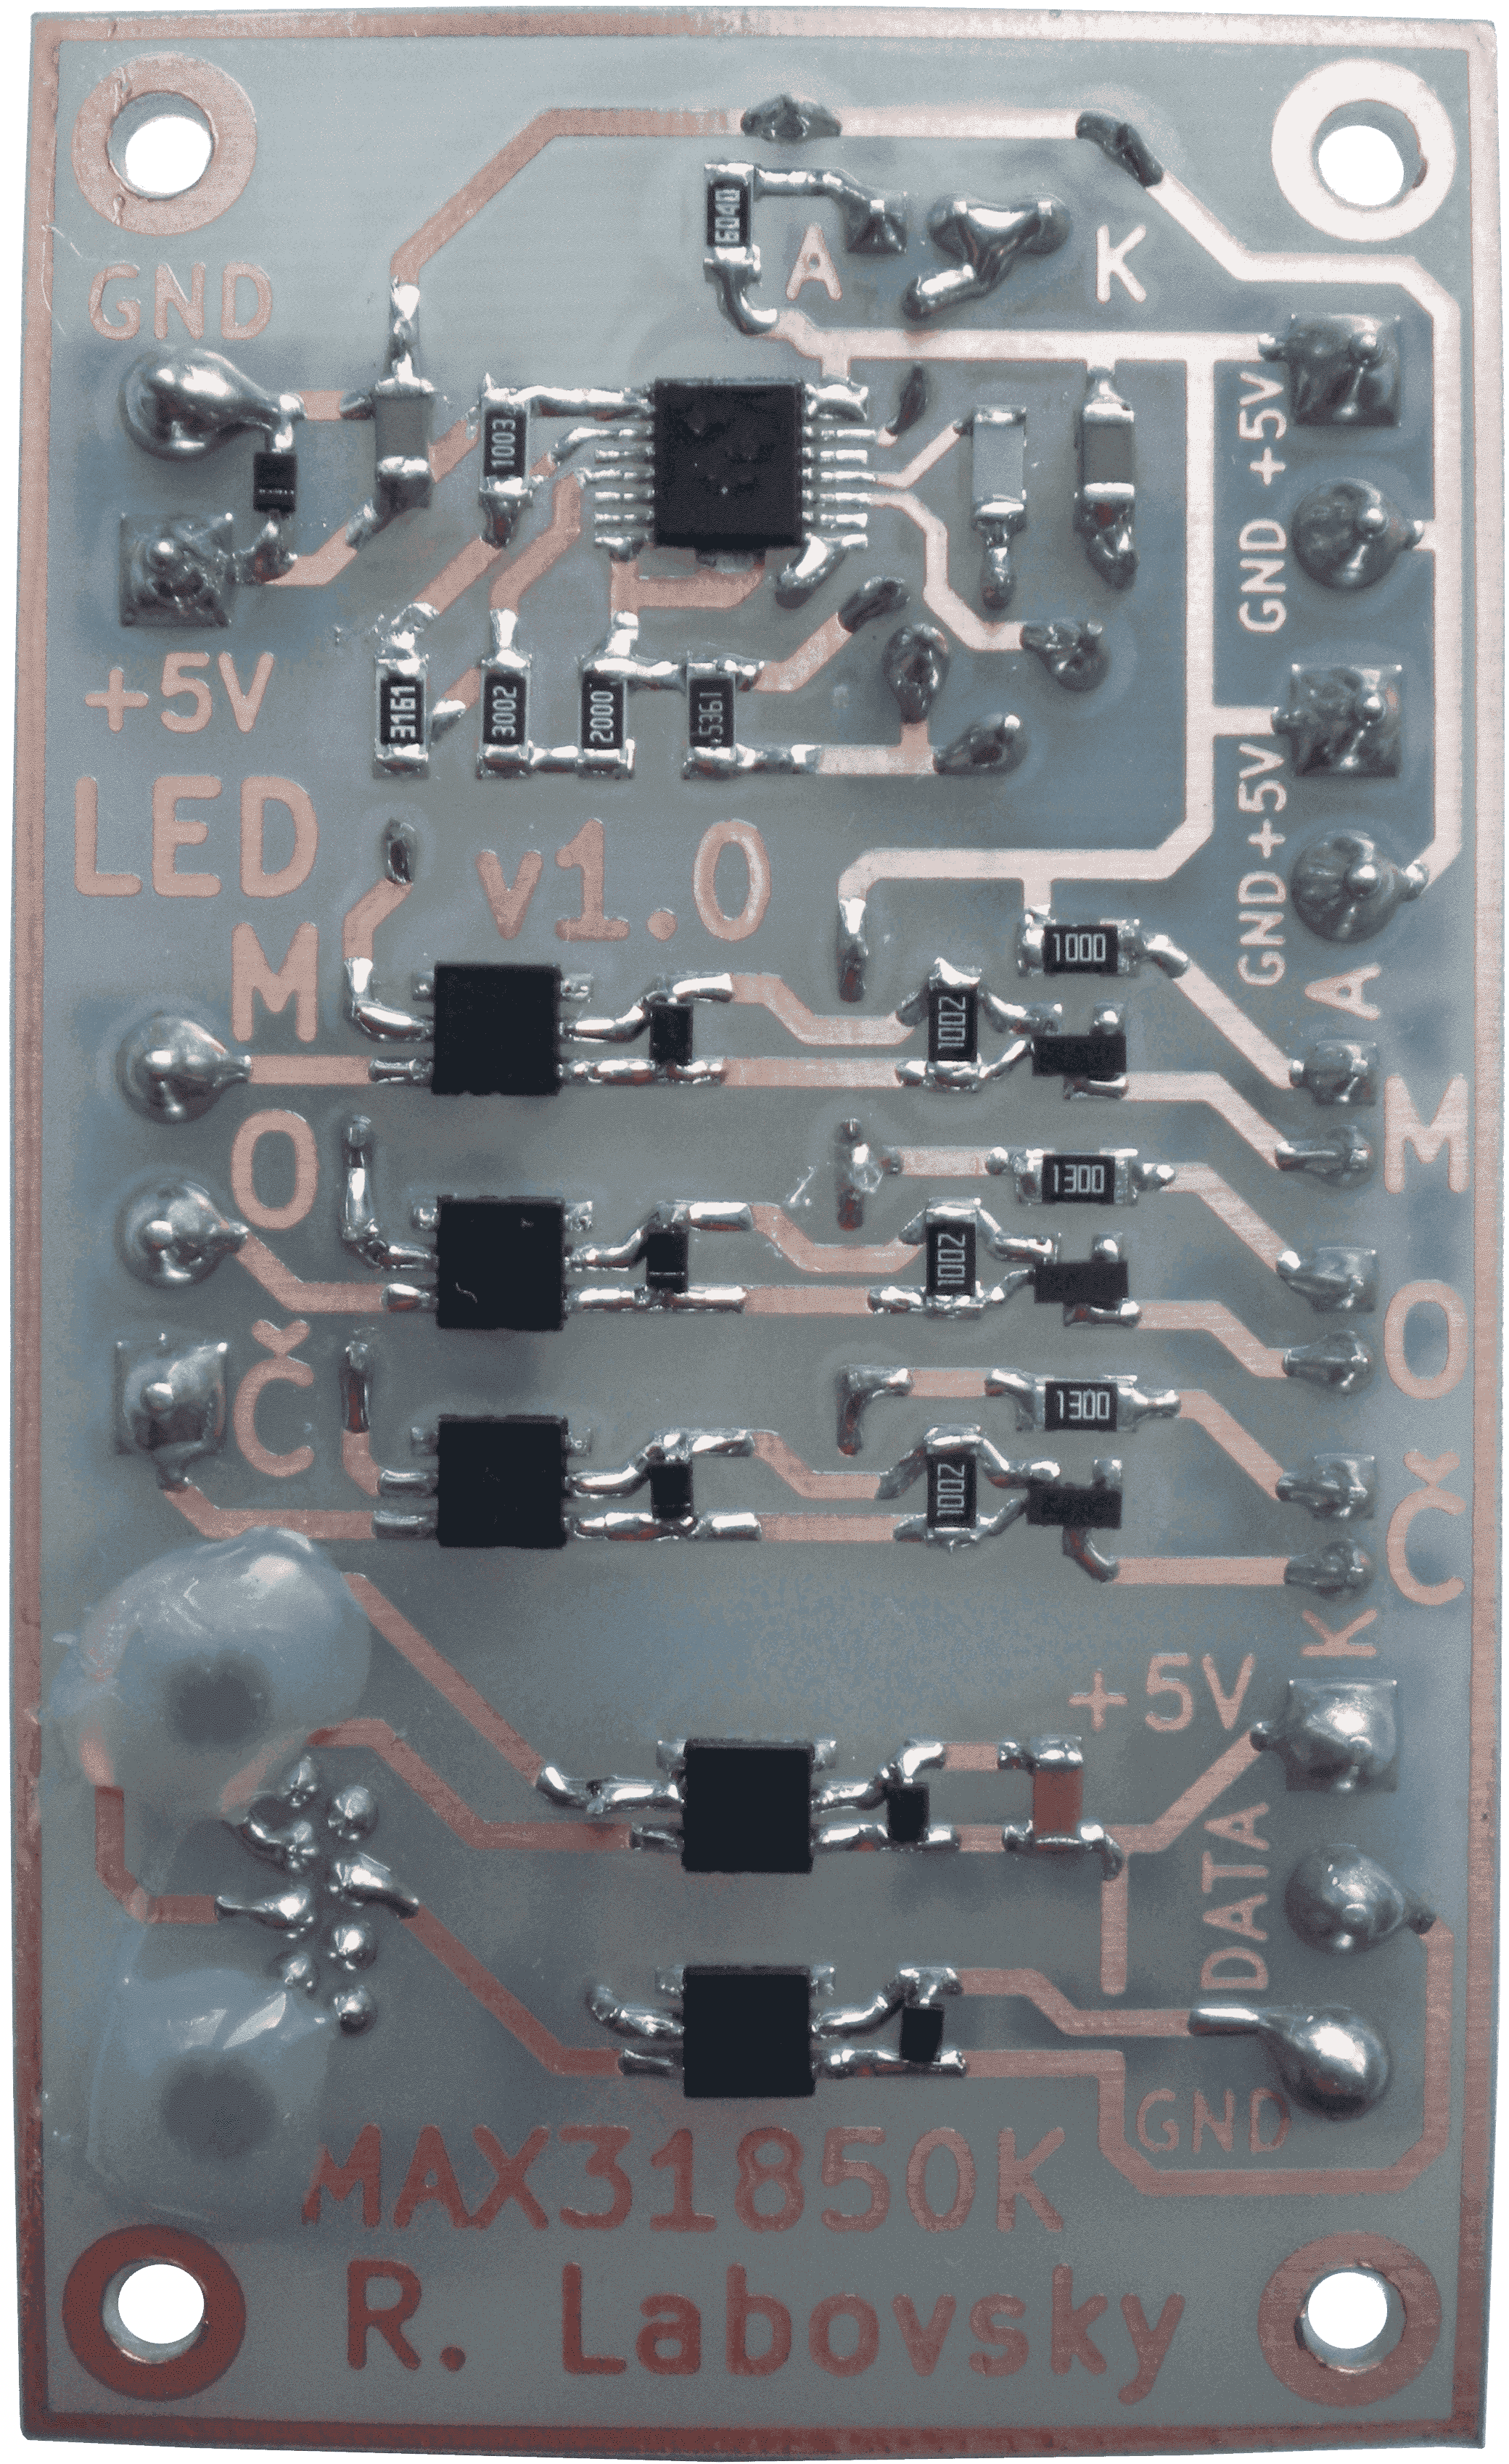
\includegraphics[width=\textwidth]{images/dps-led-ochrany-u-krbu-spodek.png}
    \caption[Spodní část DPS.]{Spodní část DPS.}
    \label{fig:dps-led-ochrany-u-krbu-spodek}
\end{figure}

\begin{figure}[H]
    \centering
    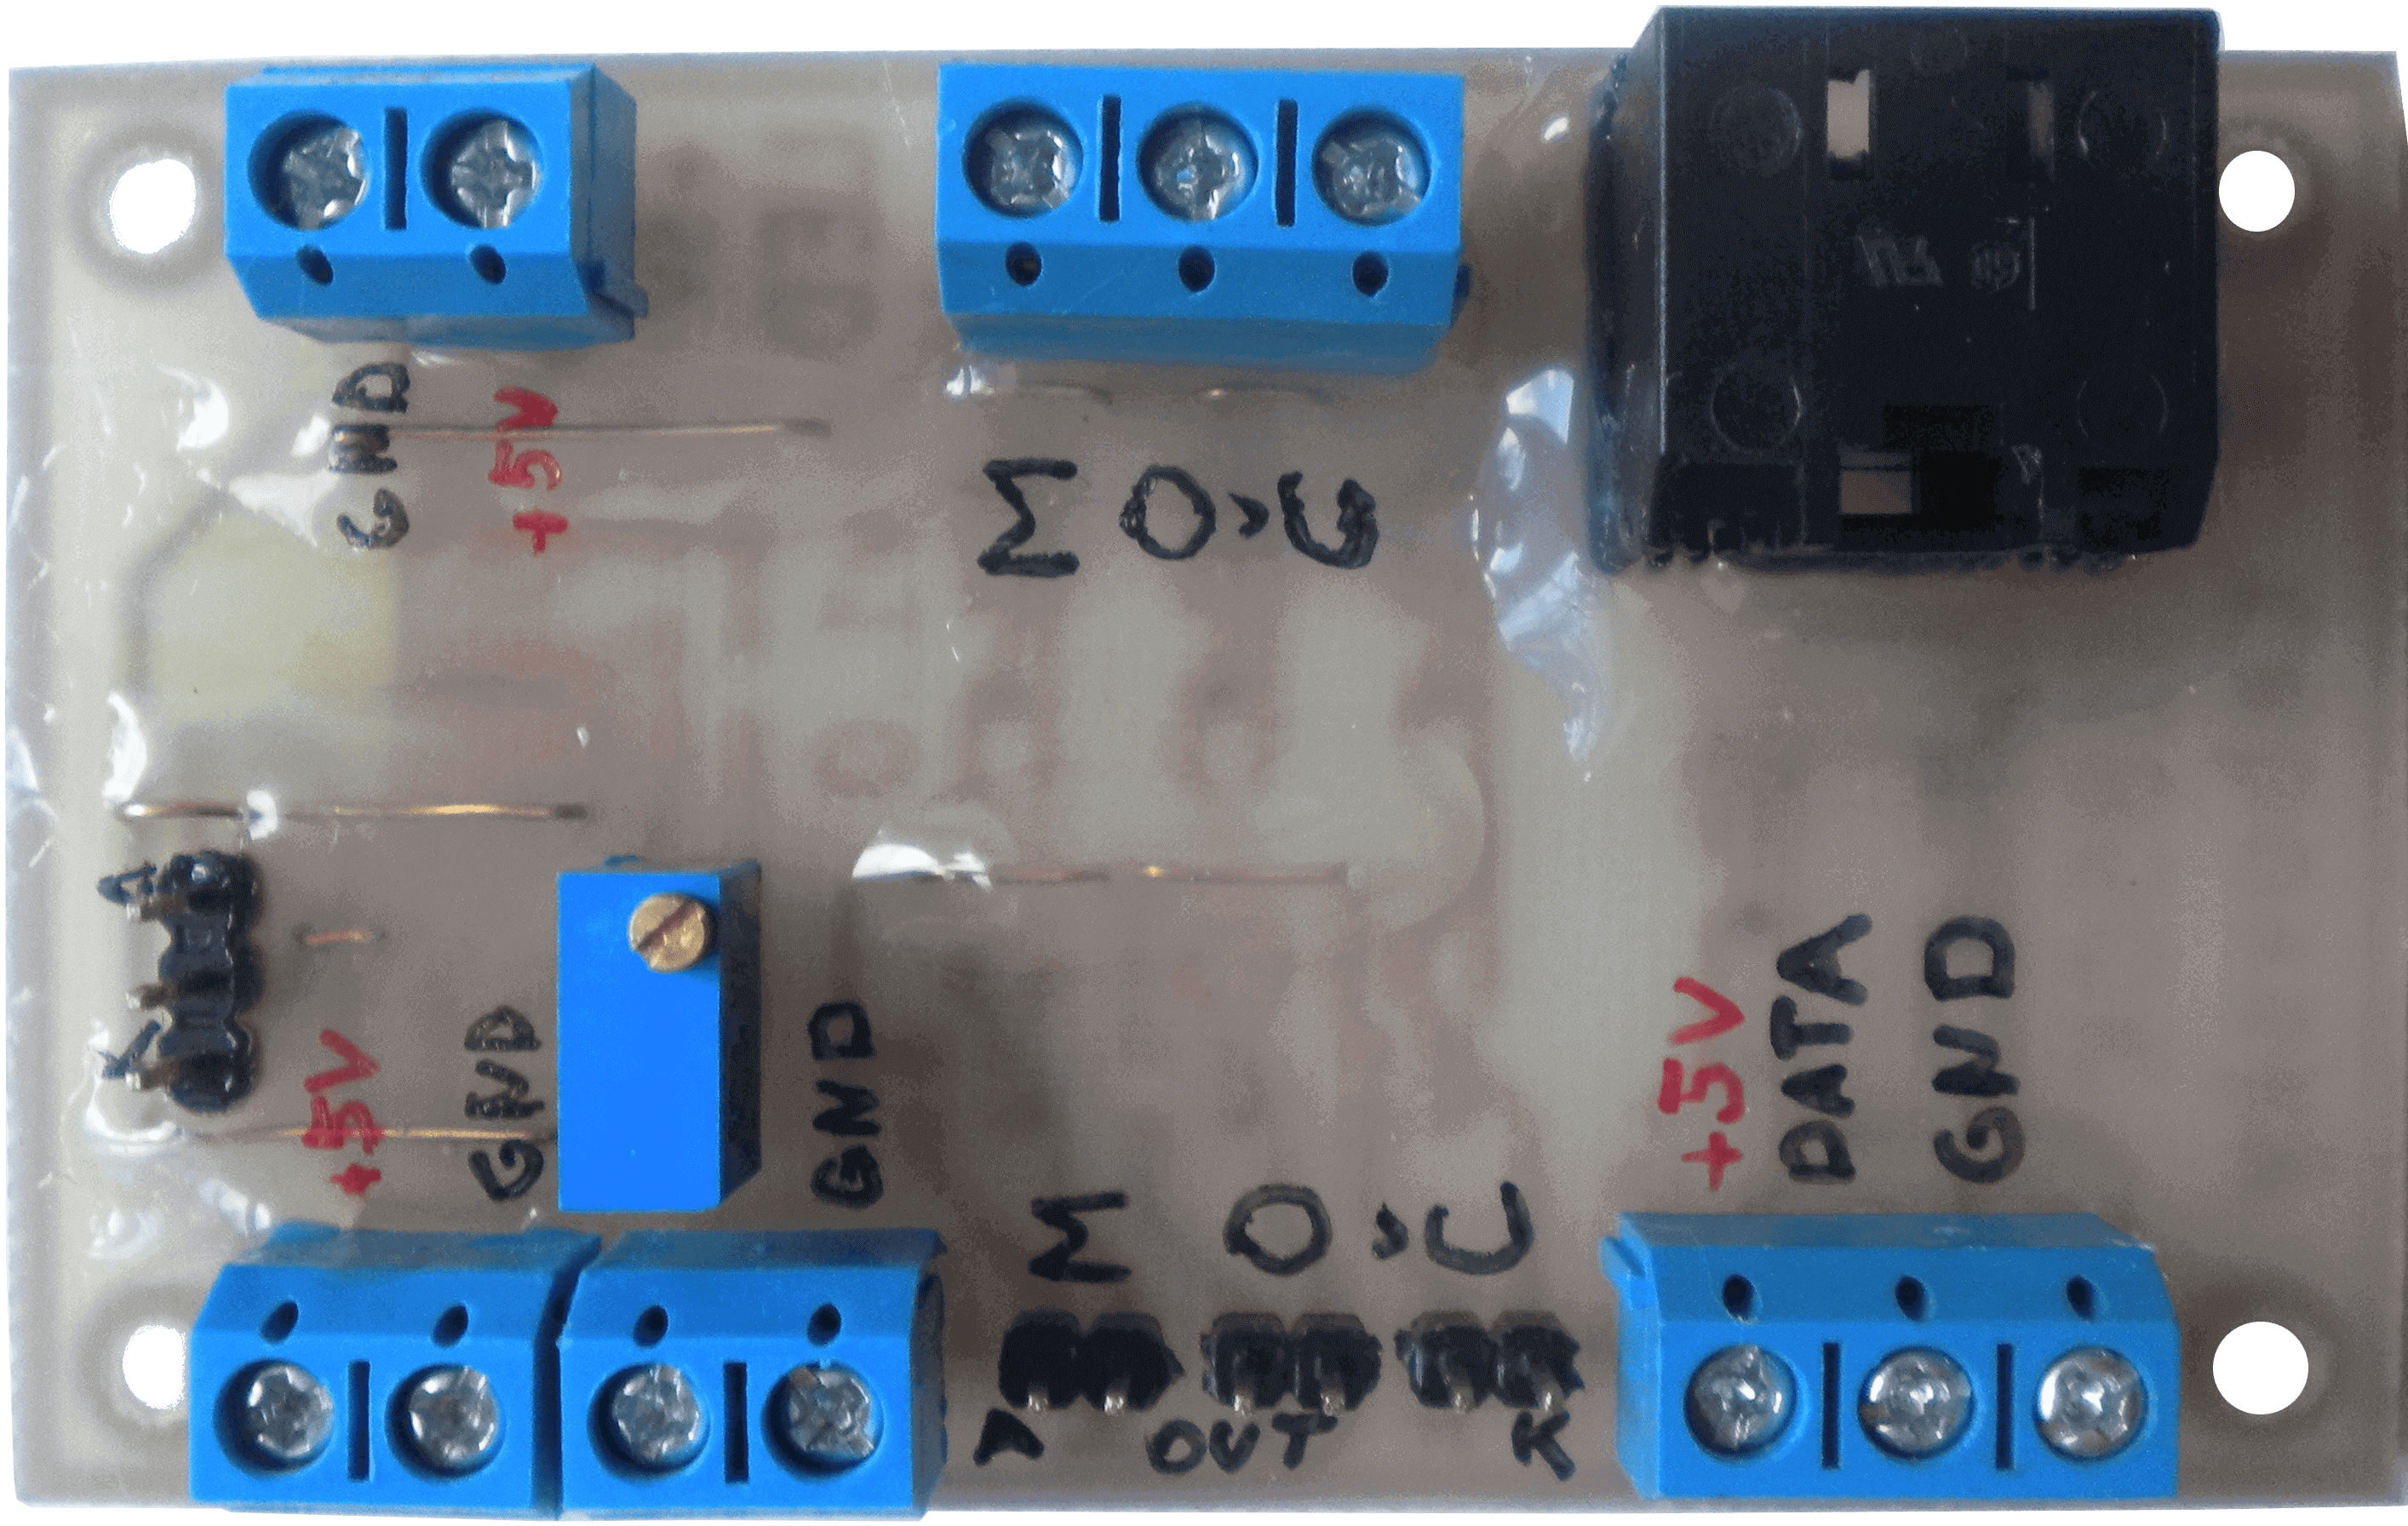
\includegraphics[width=\textwidth]{images/dps-led-ochrany-u-krbu-vrsek.png}
    \caption[Horní část DPS.]{Horní část DPS.}
    \label{fig:dps-led-ochrany-u-krbu-vrsek}
\end{figure}

\begin{figure}[H]
    \centering
    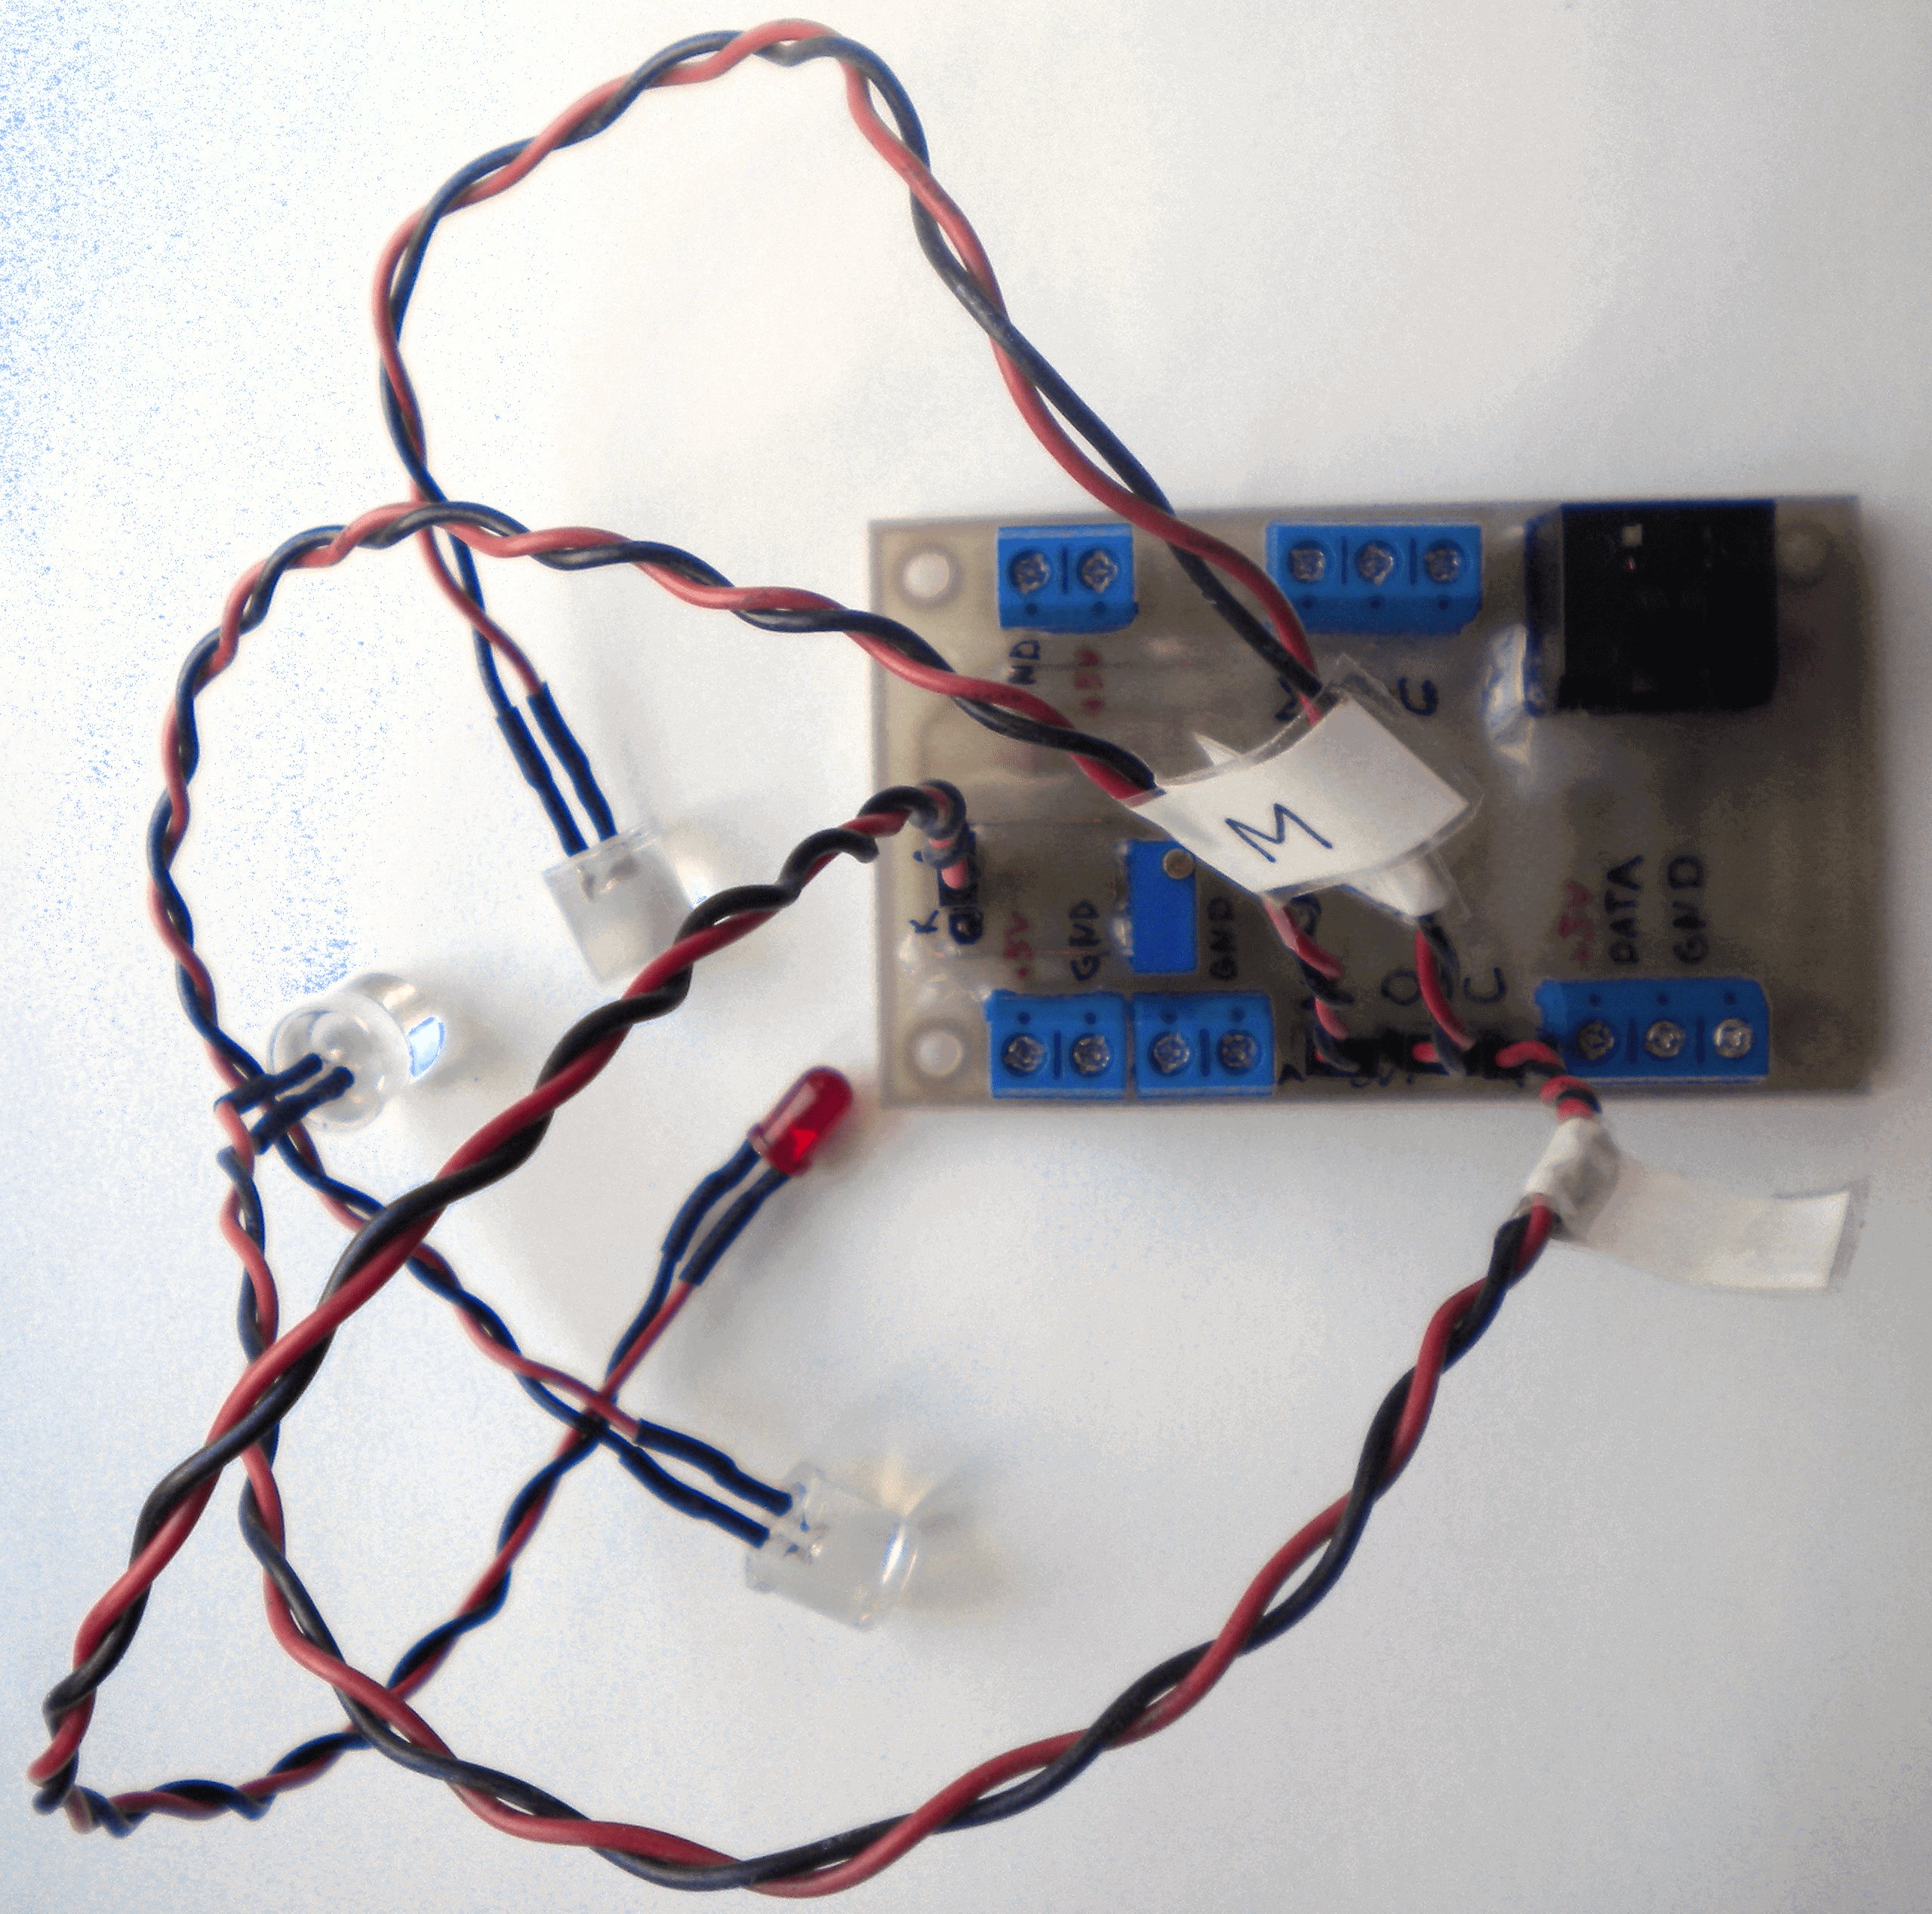
\includegraphics[width=0.95\textwidth]{images/dps-led-ochrany-u-krbu-kabely.png}
    \caption[DPS včetně signalizačních LED.]{DPS včetně signalizačních LED.}
    \label{fig:dps-led-ochrany-u-krbu-kabely}
\end{figure}

\subsubsection{Instalační krabice}
Všechna elektronika je umístěna do ochranné instalační krabice (obrázek \ref{fig:instalacni-krabice-vnitrek-krb}). Do krabice vstupují dva vodiče pro napětí 5 V a zem, tři kabely pro ovládání signalizačních LED, UTP kabel se sběrnicí 1-Wire pro teplotní senzor (termočlánek) a I$^2$C sběrnicí. Na obrázku \ref{fig:zadni-cast-krytu-vika-instalacni-krabice-krb} je zobrazena zadní část víka instalační krabice s uchycením signalizačních LED a LCD displeje. Na obrázku \ref{fig:predni-cast-krytu-vika-instalacni-krabice-krb} je přední část víka instalační krabice.

\begin{figure}[H]
    \centering
    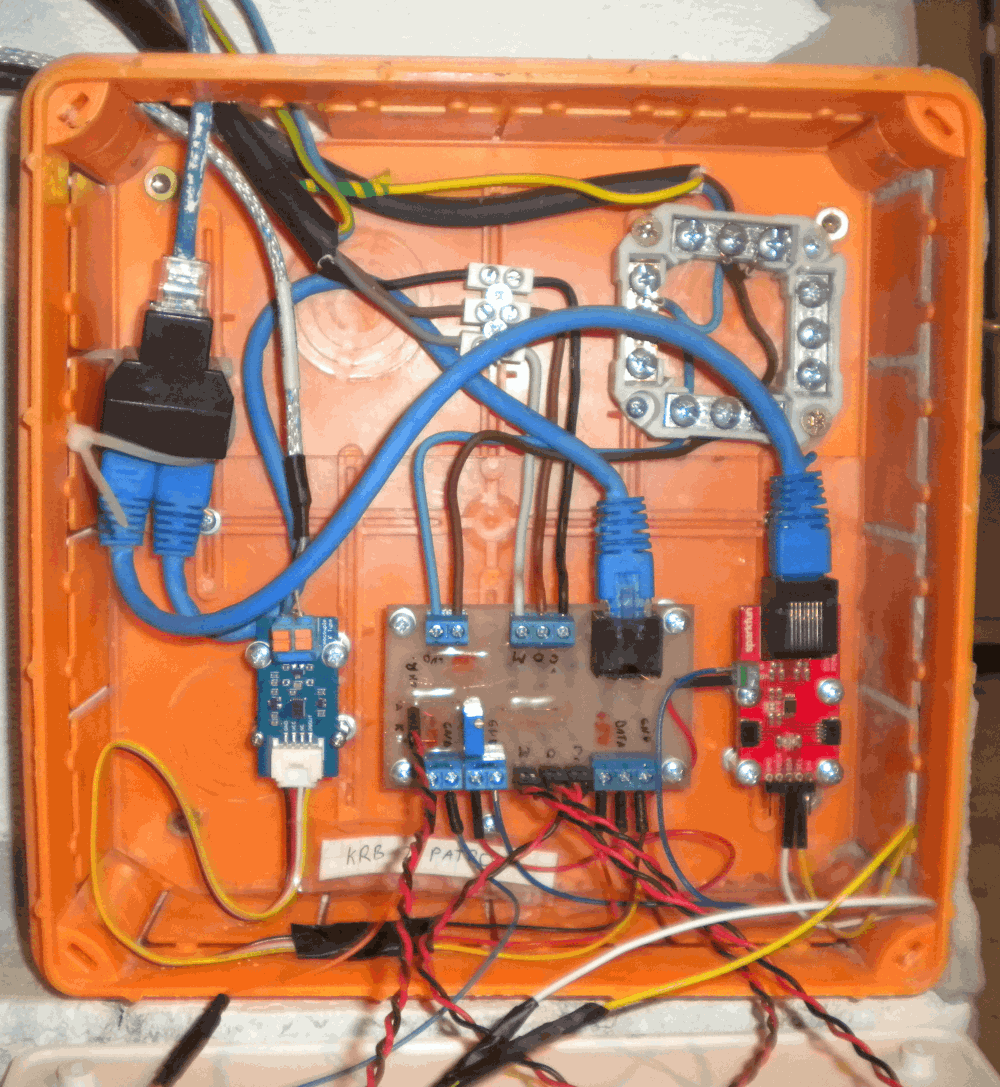
\includegraphics[width=0.6\textwidth]{images/instalacni-krabice-vnitrek-krb.png}
    \caption[Instalační krabice s jednotlivými moduly.]{Instalační krabice s jednotlivými moduly.}
    \label{fig:instalacni-krabice-vnitrek-krb}
\end{figure}

\begin{figure}[H]
    \centering
    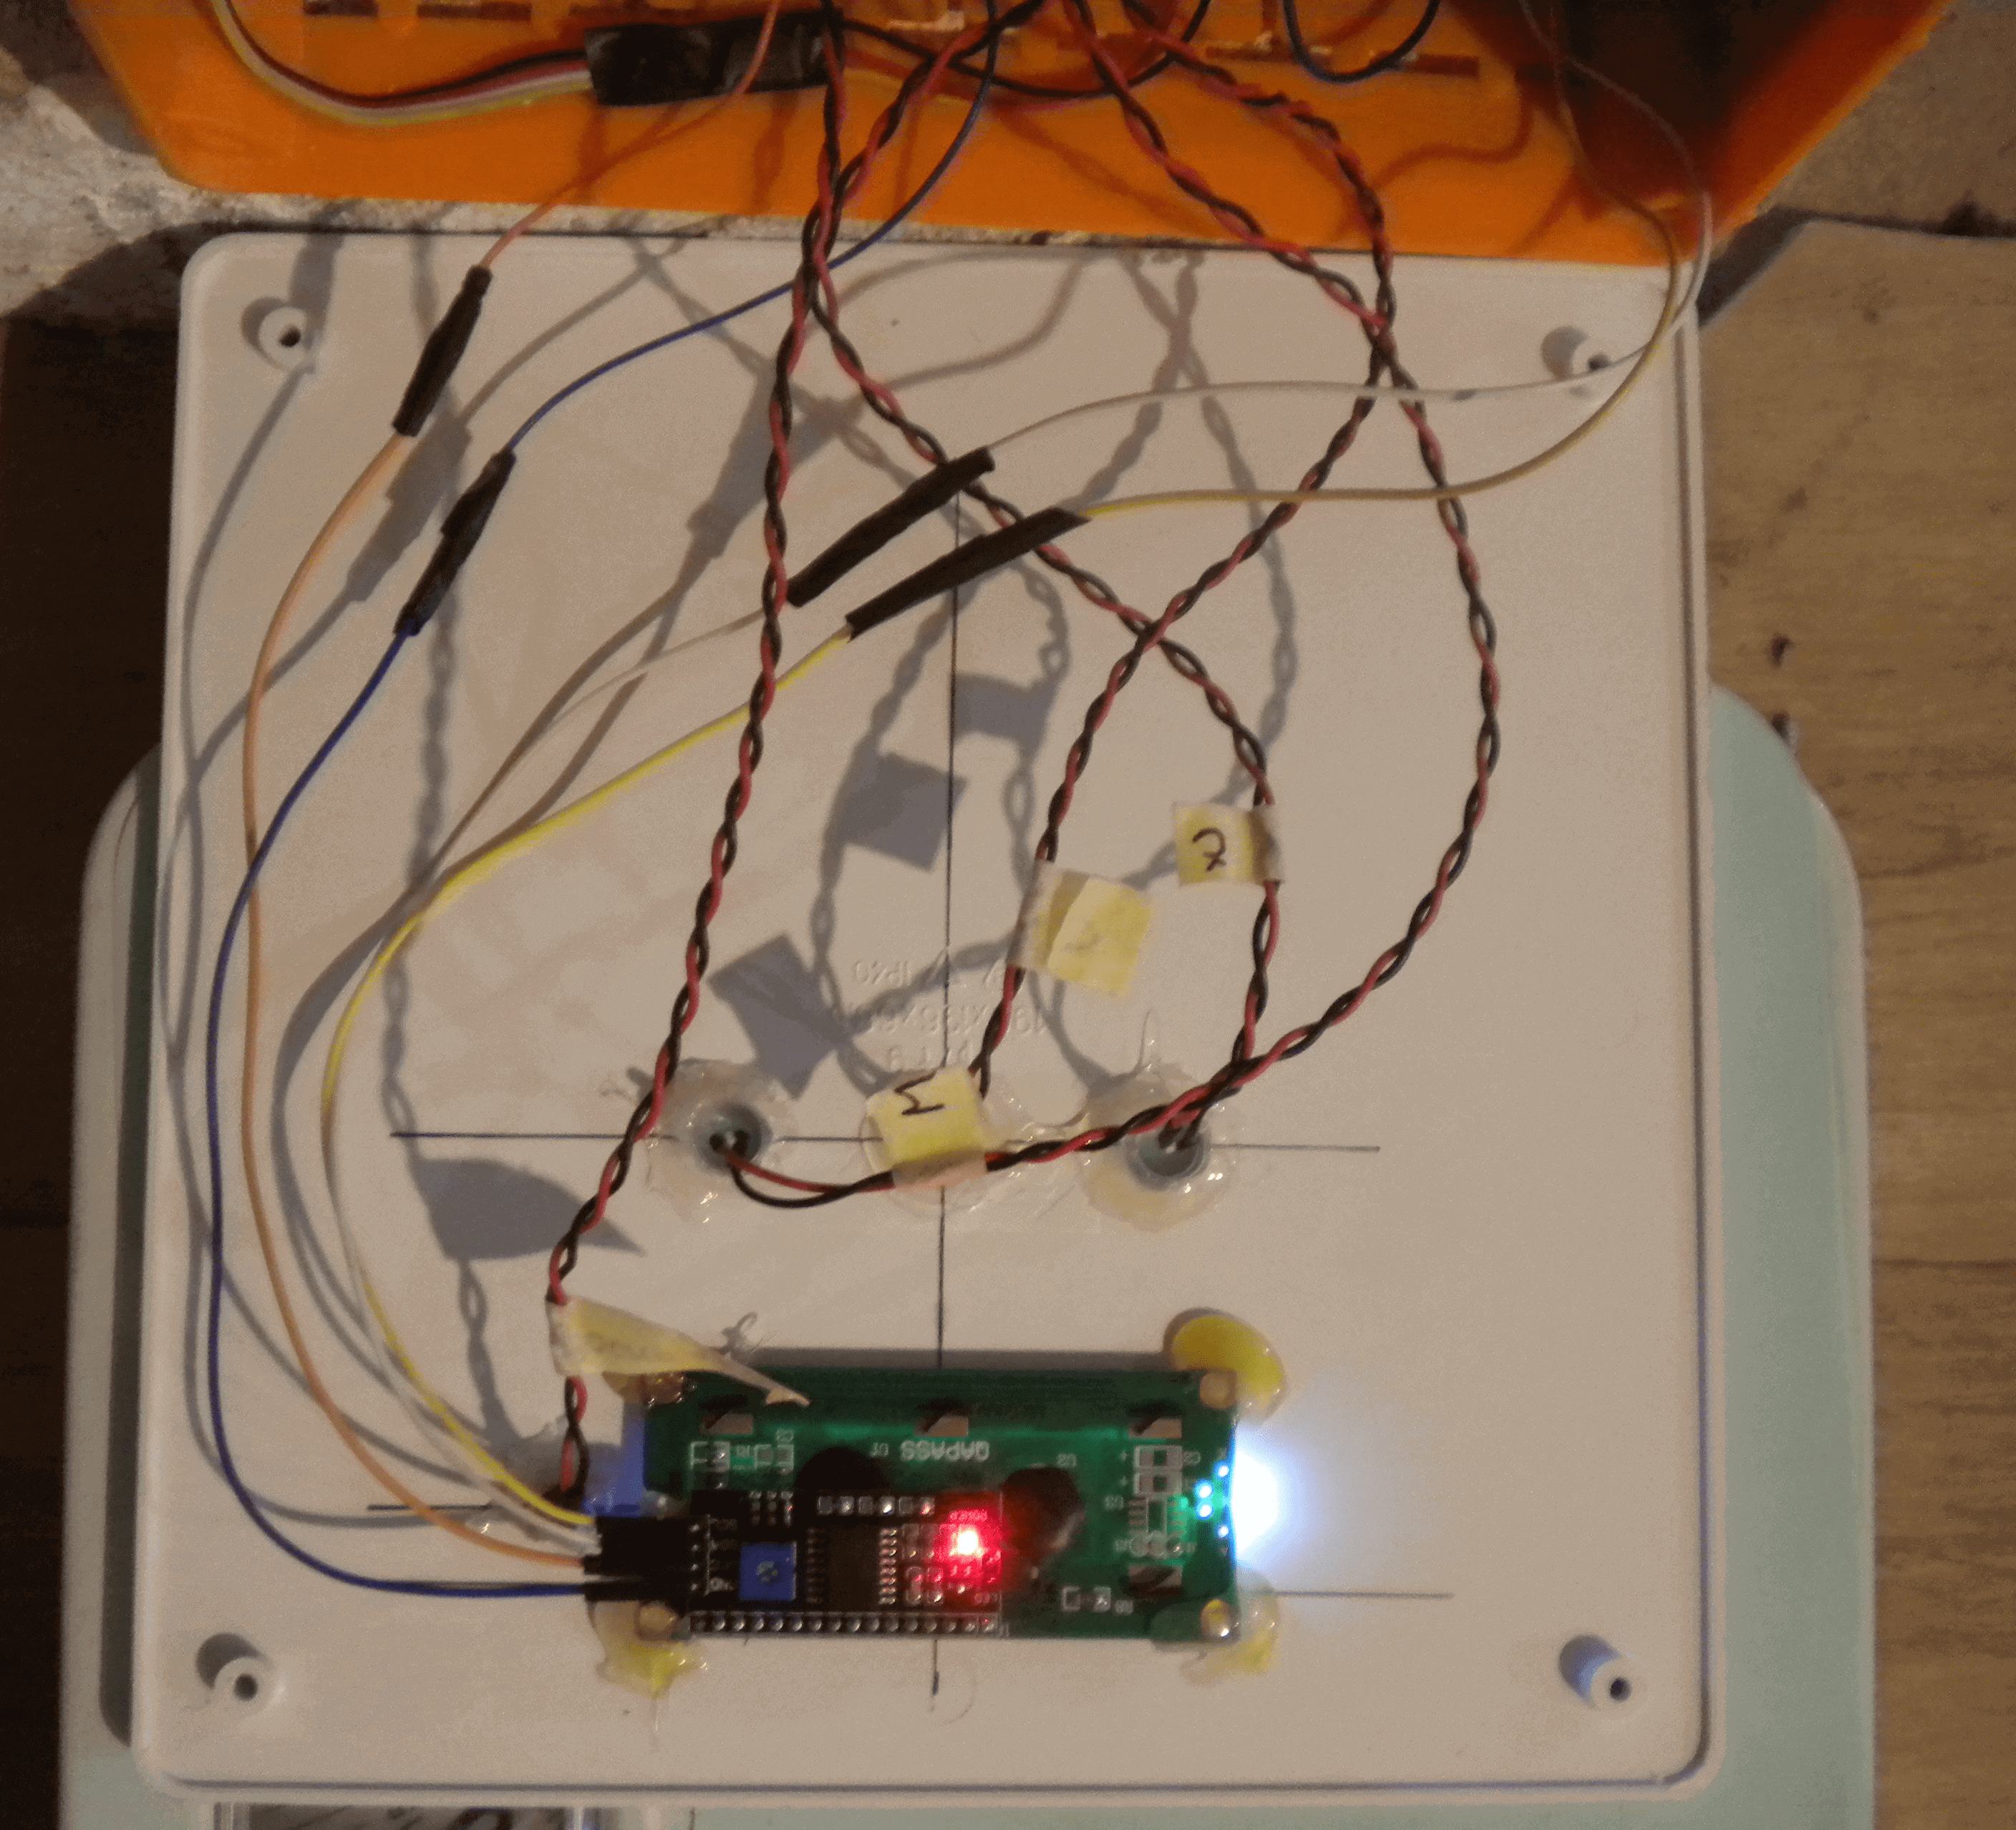
\includegraphics[width=0.6\textwidth]{images/zadni-cast-krytu-vika-instalacni-krabice-krb.png}
    \caption[Zadní část instalační krabice.]{Zadní část instalační krabice.}
    \label{fig:zadni-cast-krytu-vika-instalacni-krabice-krb}
\end{figure}

\begin{figure}[H]
    \centering
    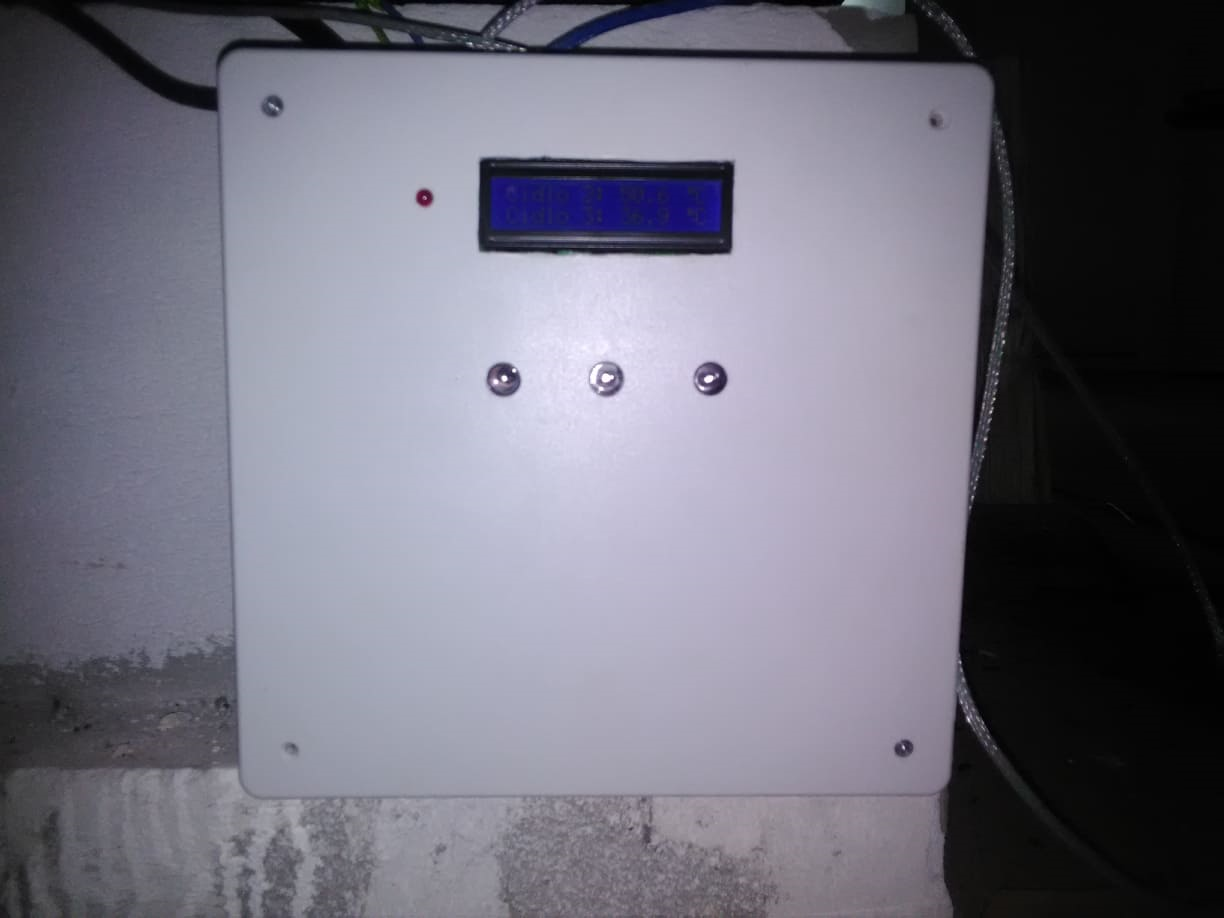
\includegraphics[width=0.6\textwidth]{images/predni-cast-krytu-vika-instalacni-krabice-krb.png}
    \caption[Víko instalační krabice.]{Víko instalační krabice. Osazený LCD displej, signalizačních LED (zleva modrá, oranžová a červená) a LED pro aktivování elektronické pojistky (červená LED vlevo od displeje).}
    \label{fig:predni-cast-krytu-vika-instalacni-krabice-krb}
\end{figure}

\section{Zónový regulátor}
Zónový regulátor se skládá s modulu PCA9615 (viz část \label{ses:i2c-sbernice} (I$^2$C)) pro realizaci I$^2$C sběrnice pomocí diferenciálních párů. Na modul je následně napojen zakoupený modul s obvodem PCA9685 od firmy NXP Semiconductors. Výstupy z modulu jsou napojeny na DPS, která zapíná/vypíná (respektive ke PWM regulaci) jednotlivé termoelektrické pohony (celkově 12 pohonů, každý je řízen samostatně), čímž dochází k regulaci otopné vody do otopných okruhů.

\subsubsection{Modul s PCA9685}
Modul s obvodem PCA9685 umožňuje pomocí I$^2$C sběrnice ovládat 16 výstupů se stejnou individuální hodnotou PWM (se střídou 0\% až 100 \%), frekvence je programovatelná od 24 Hz do 1\,526 Hz. Každý kanál navíc může dodat 10~mA jako source, případně 25 mA jako sink (což je 160 mA respektive 400 mA celkově).

\begin{figure}[H]
    \centering
    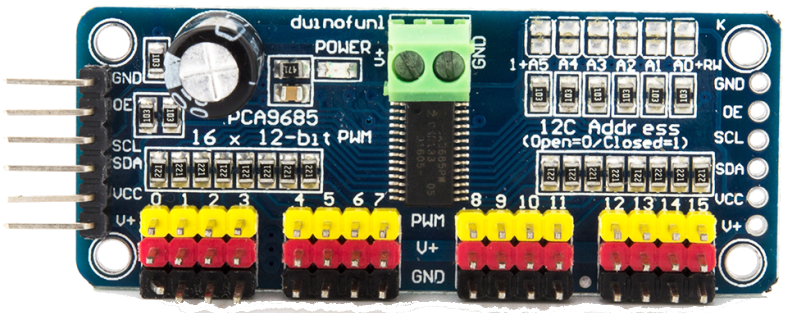
\includegraphics[width=0.8\textwidth]{images/modul-pca9685-pwm-regulace.png}
    \caption[Modul s obvodem PCA9685.]{Modul s obvodem PCA9685 \cite{modul-pca9685}.}
    \label{fig:modul-pca9685-pwm-regulace}
\end{figure}
\subsubsection{DPS pro ovládání termoelektrických pohonů}
Termoelektrické pohony jsou ovládány na základě hodnoty PWM z modulu PCA9685 (viz předchozí bod), každý výstupu ovládá jednotlivý pohon. Vzhledem k tomu, že termoelektrické pohony jsou na stejnosměrné napětí 24 V, je nutné využít napěťový převodník z 5 V na 24 V. K tomu slouží tranzistor MOSFET (DMN3023L-7). V závislosti na hodnotě PWM na jeho vstupu (gate) je otevírán/zavírán a dochází tak k regulaci napětí/proudu v~termoelektrickém pohonu, který je zapojen jako zátěž (přes drain). Paralelně k~tranzistoru se nachází přepínač, který slouží v případě poruchy k manuálnímu zapnutí/vypnutí pohonu. Přepínač má jmenovitý proud 0,5~A, což je dostatečné pro termoelektrický pohon, kterým při zapnutí teče maximální proud 250 mA (následně dochází ke snižování a saturaci proudu). Každý kanál obsahuje zelenou LED pro signalizaci, zda dochází k ovládání pomocí PWM. Maximální proud procházející zelenou LED je 7 mA, což je v~mezích pro obvod PCA9685, kde je uváděno, že pro každý kanál je maximální proud 10 mA. Jak již bylo řečeno pohony jsou napájeny pomocí 24 V, jsou vytvořené dvě napájecí větve s obvodem TPC26600 (popsaný v části \ref{sec:napajeni-1-wire-sbernice}), rozdíl spočívá ve vstupním napájení, které činí 24 V. Jsou tedy rozdílné i~maximální a~minimální povolené meze, které činí max. 24,25 V a min. 23,75~V. Dále každá větev má nastavený maximální proud 1,5 A (každý pohon má maximální hodnotu proudu při zapnutí 250 mA pro celkově 6 pohonů na větev). Vzhledem k jednoduchosti obvodu TPS26600 a k jeho vlastnostem (především pro automatickou detekci odstranění závady, bez nutnosti restartu zařízení) bylo raději zvoleno zapojení se dvěma větvemi (maximální proud pro TPS26600 činí 2,21 A) než využití jiného integrovaného obvodu pro sloučení do jedné větve. Na obrázku \ref{fig:dps-zonovy-regulator} je navržená DPS zónového regulátoru, která v současné době není vyrobená.


\begin{figure}[H]
    \centering
    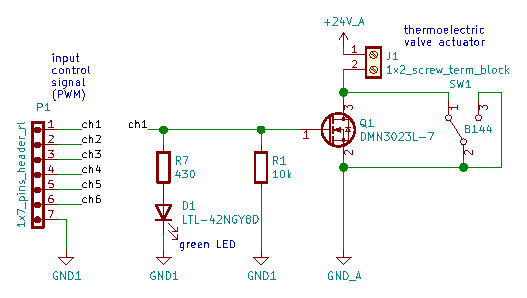
\includegraphics[width=\textwidth]{images/svg/kicad/zonovy-regulator-mosfet-pwm.eps}
    \caption[Zapojení jednoho kanálu pro ovládání termoelektrického pohonu.]{Zapojení jednoho kanálu pro ovládání termoelektrického pohonu.}
    \label{fig:zonovy-regulator-mosfet-pwm}
\end{figure}


\begin{figure}[H]
    \centering
    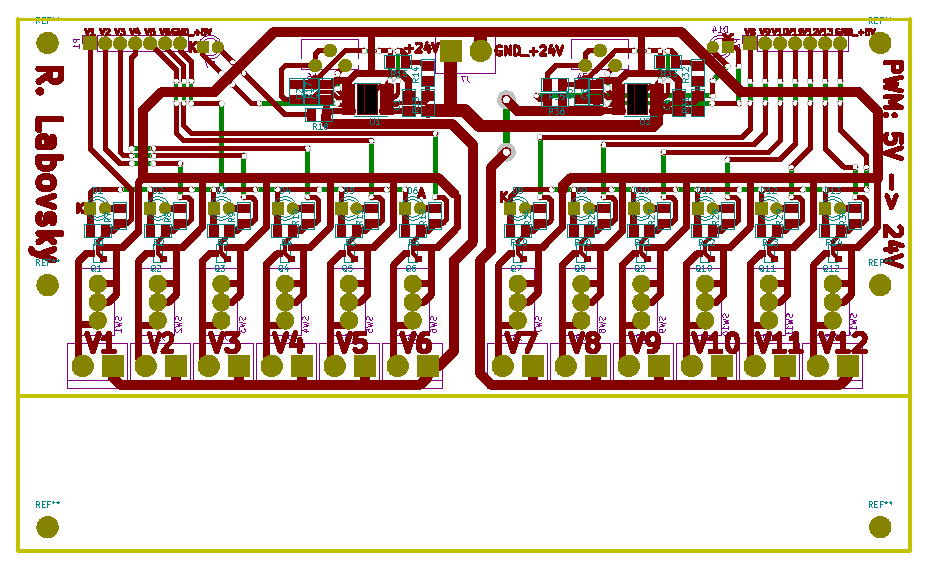
\includegraphics[width=\textwidth]{images/svg/kicad/dps-zonovy-regulator.eps}
    \caption[Navržená DPS pro zónový regulátor.]{Navržená DPS pro zónový regulátor. Rozměry jsou 151 mm × 90 mm.}
    \label{fig:dps-zonovy-regulator}
\end{figure}

\subsubsection{Termoelektrické pohony Salus T30NC}  
Termoelektrický pohon Salus T30NC slouží k ovládání ventilů pro jednotlivé otopné okruhy. Je napájen stejnosměrným napětí 24 V při maximálním proudovém odběru při zapnutí 250 mA. Provozní příkon jsou 2 W. Rozměr závitu je M30\,×\,1,5. Maximální délka zdvihu pro dřík ventilu činí 4 mm. Síla pohonu je 100 N ($\pm$10 \%). Čas pro otevření je přibližně 2 minuty. Jedná se o~typ \acrshort{nc} (\textit{\acrlong{nc}}), při odpojení napájení je ventily zavřen. Pohon má funkci „First Open“ neboli je možné pomocí zarážky ventil instalovat jako otevřený bez nutnosti napájení (využít v případě, kdy není ještě instalovaná centrální jednotka).

\begin{figure}[H]
    \centering
    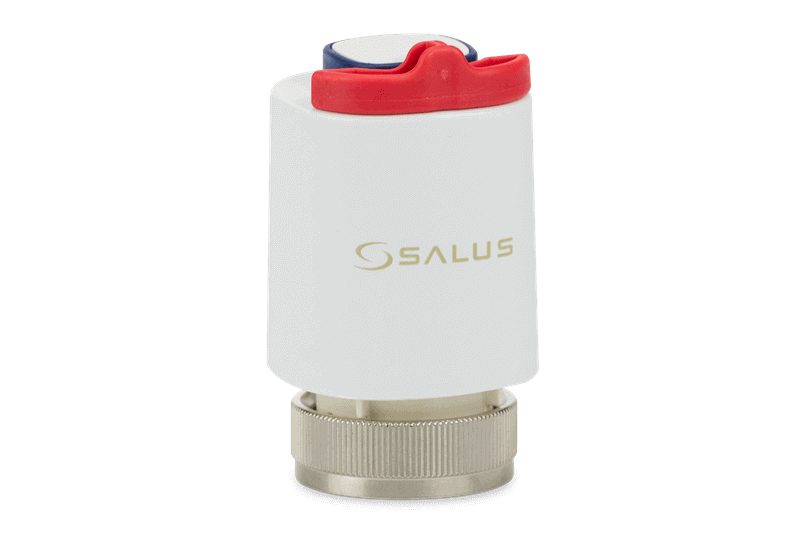
\includegraphics[width=0.8\textwidth]{images/termoelektricky-pohon-salus-t30nc-24-v.png}
    \caption[Termoelektrický pohon Salus T30NC na stejnosměrné napětí 24 V.]{Termoelektrický pohon Salus T30NC na stejnosměrné napětí 24~V \cite{termoelektricky-pohon-t30nc}.}
    \label{fig:termoelektricky-pohon-salus-t30nc-24-v}
\end{figure}

\section{Digitální chodbové termostaty}
\label{digitalni-chodbove-termostaty}
Pro snímání teplot z jednotlivých pater na chodbách slouží digitální termostat s označením W3230. Termostat disponuje jedním spínací výstupem (v případě potřeby vytápění se výstup sepne, jinak je rozepnut). Je možné nastavit hysterezi, časové zpoždění, kalibraci teploty a rozsah maximálních teplot. Lze také aktivovat signalizaci, která se spustí po dosažení maximální přípustné teploty. Pro napájení je potřeba stejnosměrné napětí 12 V. Pro snímání teploty slouží NTC termistor. Rozsah teplot je -40 °C až 120 °C. Přesnost měření je $\pm$ 0,1 °C. Termostat lze nahradit za jakýkoliv jiný, který disponuje spínacím výstupem.


\begin{figure}[H]
    \centering
    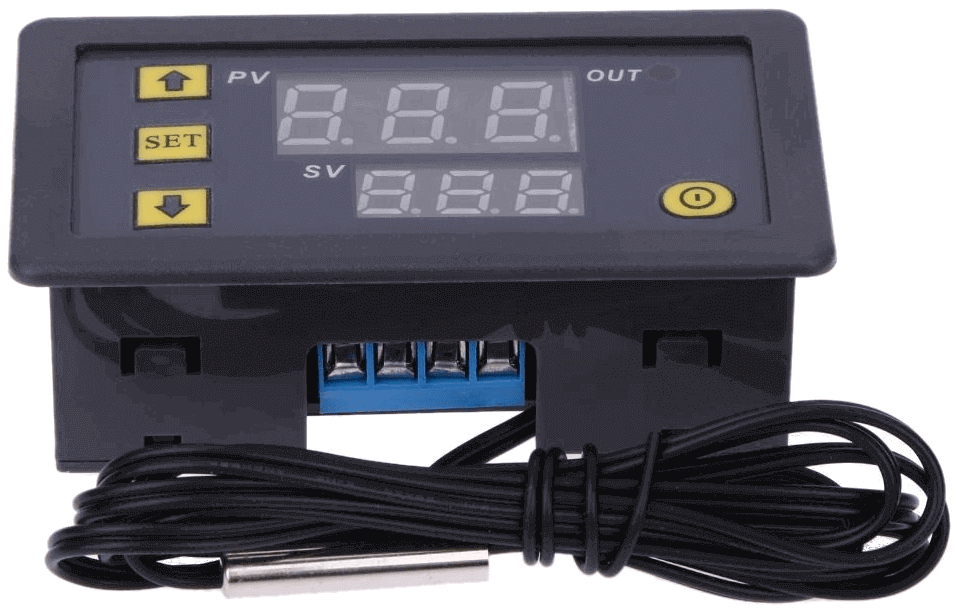
\includegraphics[width=0.8\textwidth]{images/digitalni-termostat-w3230.png}
    \caption[Digitální termostat W3230.]{Digitální termostat W3230 \cite{digitalni-termostat-w3230}.}
    \label{fig:digitalni-termostat-w3230}
\end{figure}


\section{Spínací jednotka}
Pro spínání čerpadel a signalizačních LED slouží dva zakoupené relé moduly po čtyrech kanálech. Relé umožňují spínat výkony 250 VAC při max. 10~A a 30 V DC při max. 10~A. Jednotlivé kanály jsou oddělené galvanicky (dále je vyfrézovaná část DPS mezi výkonovou částí a spínací částí), též je možné využít různých zdrojů pro napájení spínací části a napájení relé. Zapojení jednoho kanálu je obrázku \ref{fig:rele-modul-jeden-kanal}. Celý relé modul je na obrázku \ref{fig:ctyr-kanalovy-rele-modul}.

\begin{figure}[H]
    \centering
    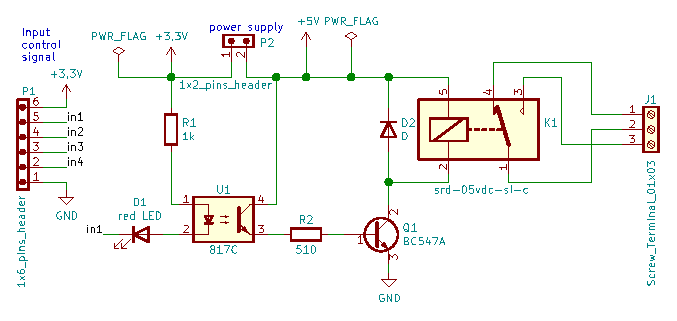
\includegraphics[width=\textwidth]{images/svg/kicad/rele-modul-jeden-kanal.eps}
    \caption[Zapojení jednoho kanálu relé modulu.]{Zapojení jednoho kanálu relé modulu.}
    \label{fig:rele-modul-jeden-kanal}
\end{figure}


\begin{figure}[H]
    \centering
    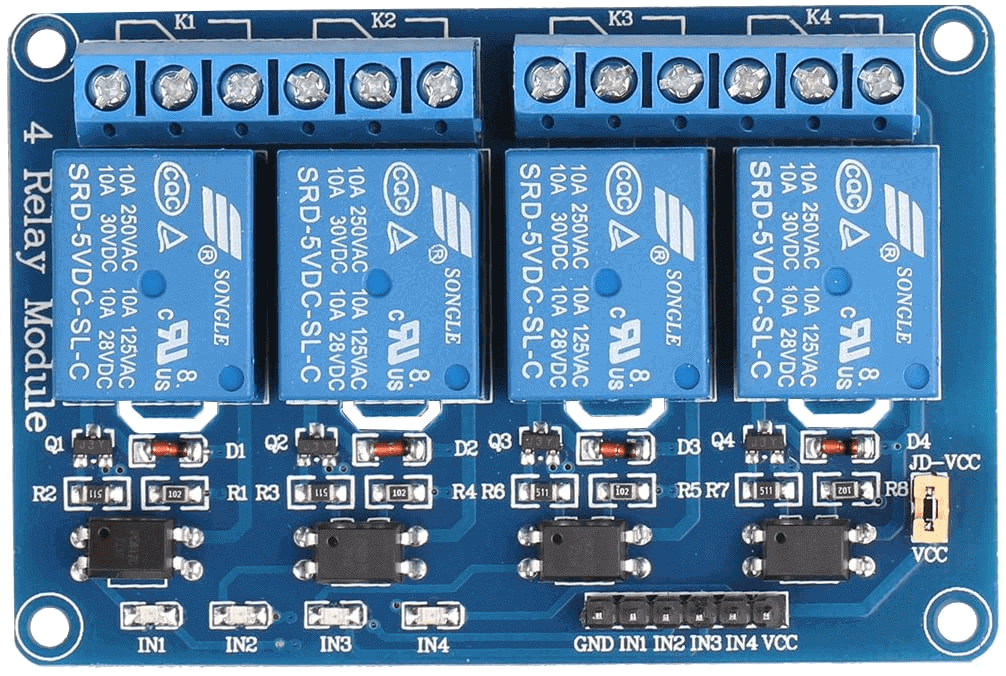
\includegraphics[width=0.8\textwidth]{images/ctyr-kanalovy-rele-modul.png}
    \caption[Čtyř kanálový relé modul.]{Čtyř kanálový relé modul \cite{ctyr-kanalovy-rele-modul}.}
    \label{fig:ctyr-kanalovy-rele-modul}
\end{figure}

\section{Realizovaný rozvaděč s elektronikou}

V realizovaném rozvaděči na obrázku \ref{fig:rozvadec-ve-sklepe-s-elektronikou} je umístěn 5 V zdroj pro napájení centrální jednotky, relé modulů, I$^2$C diferenciální sběrnice, napájení 1-Wire sběrnice a napájení elektroniky u krbů. Dále je zde 12 V zdroj pro napájení dvou lokálních chodbových termostatů. V  neposlední době jsou zde jističe pro jednotlivé zdroje a čerpadla včetně proudového chrániče.

\begin{figure}[H]
    \centering
    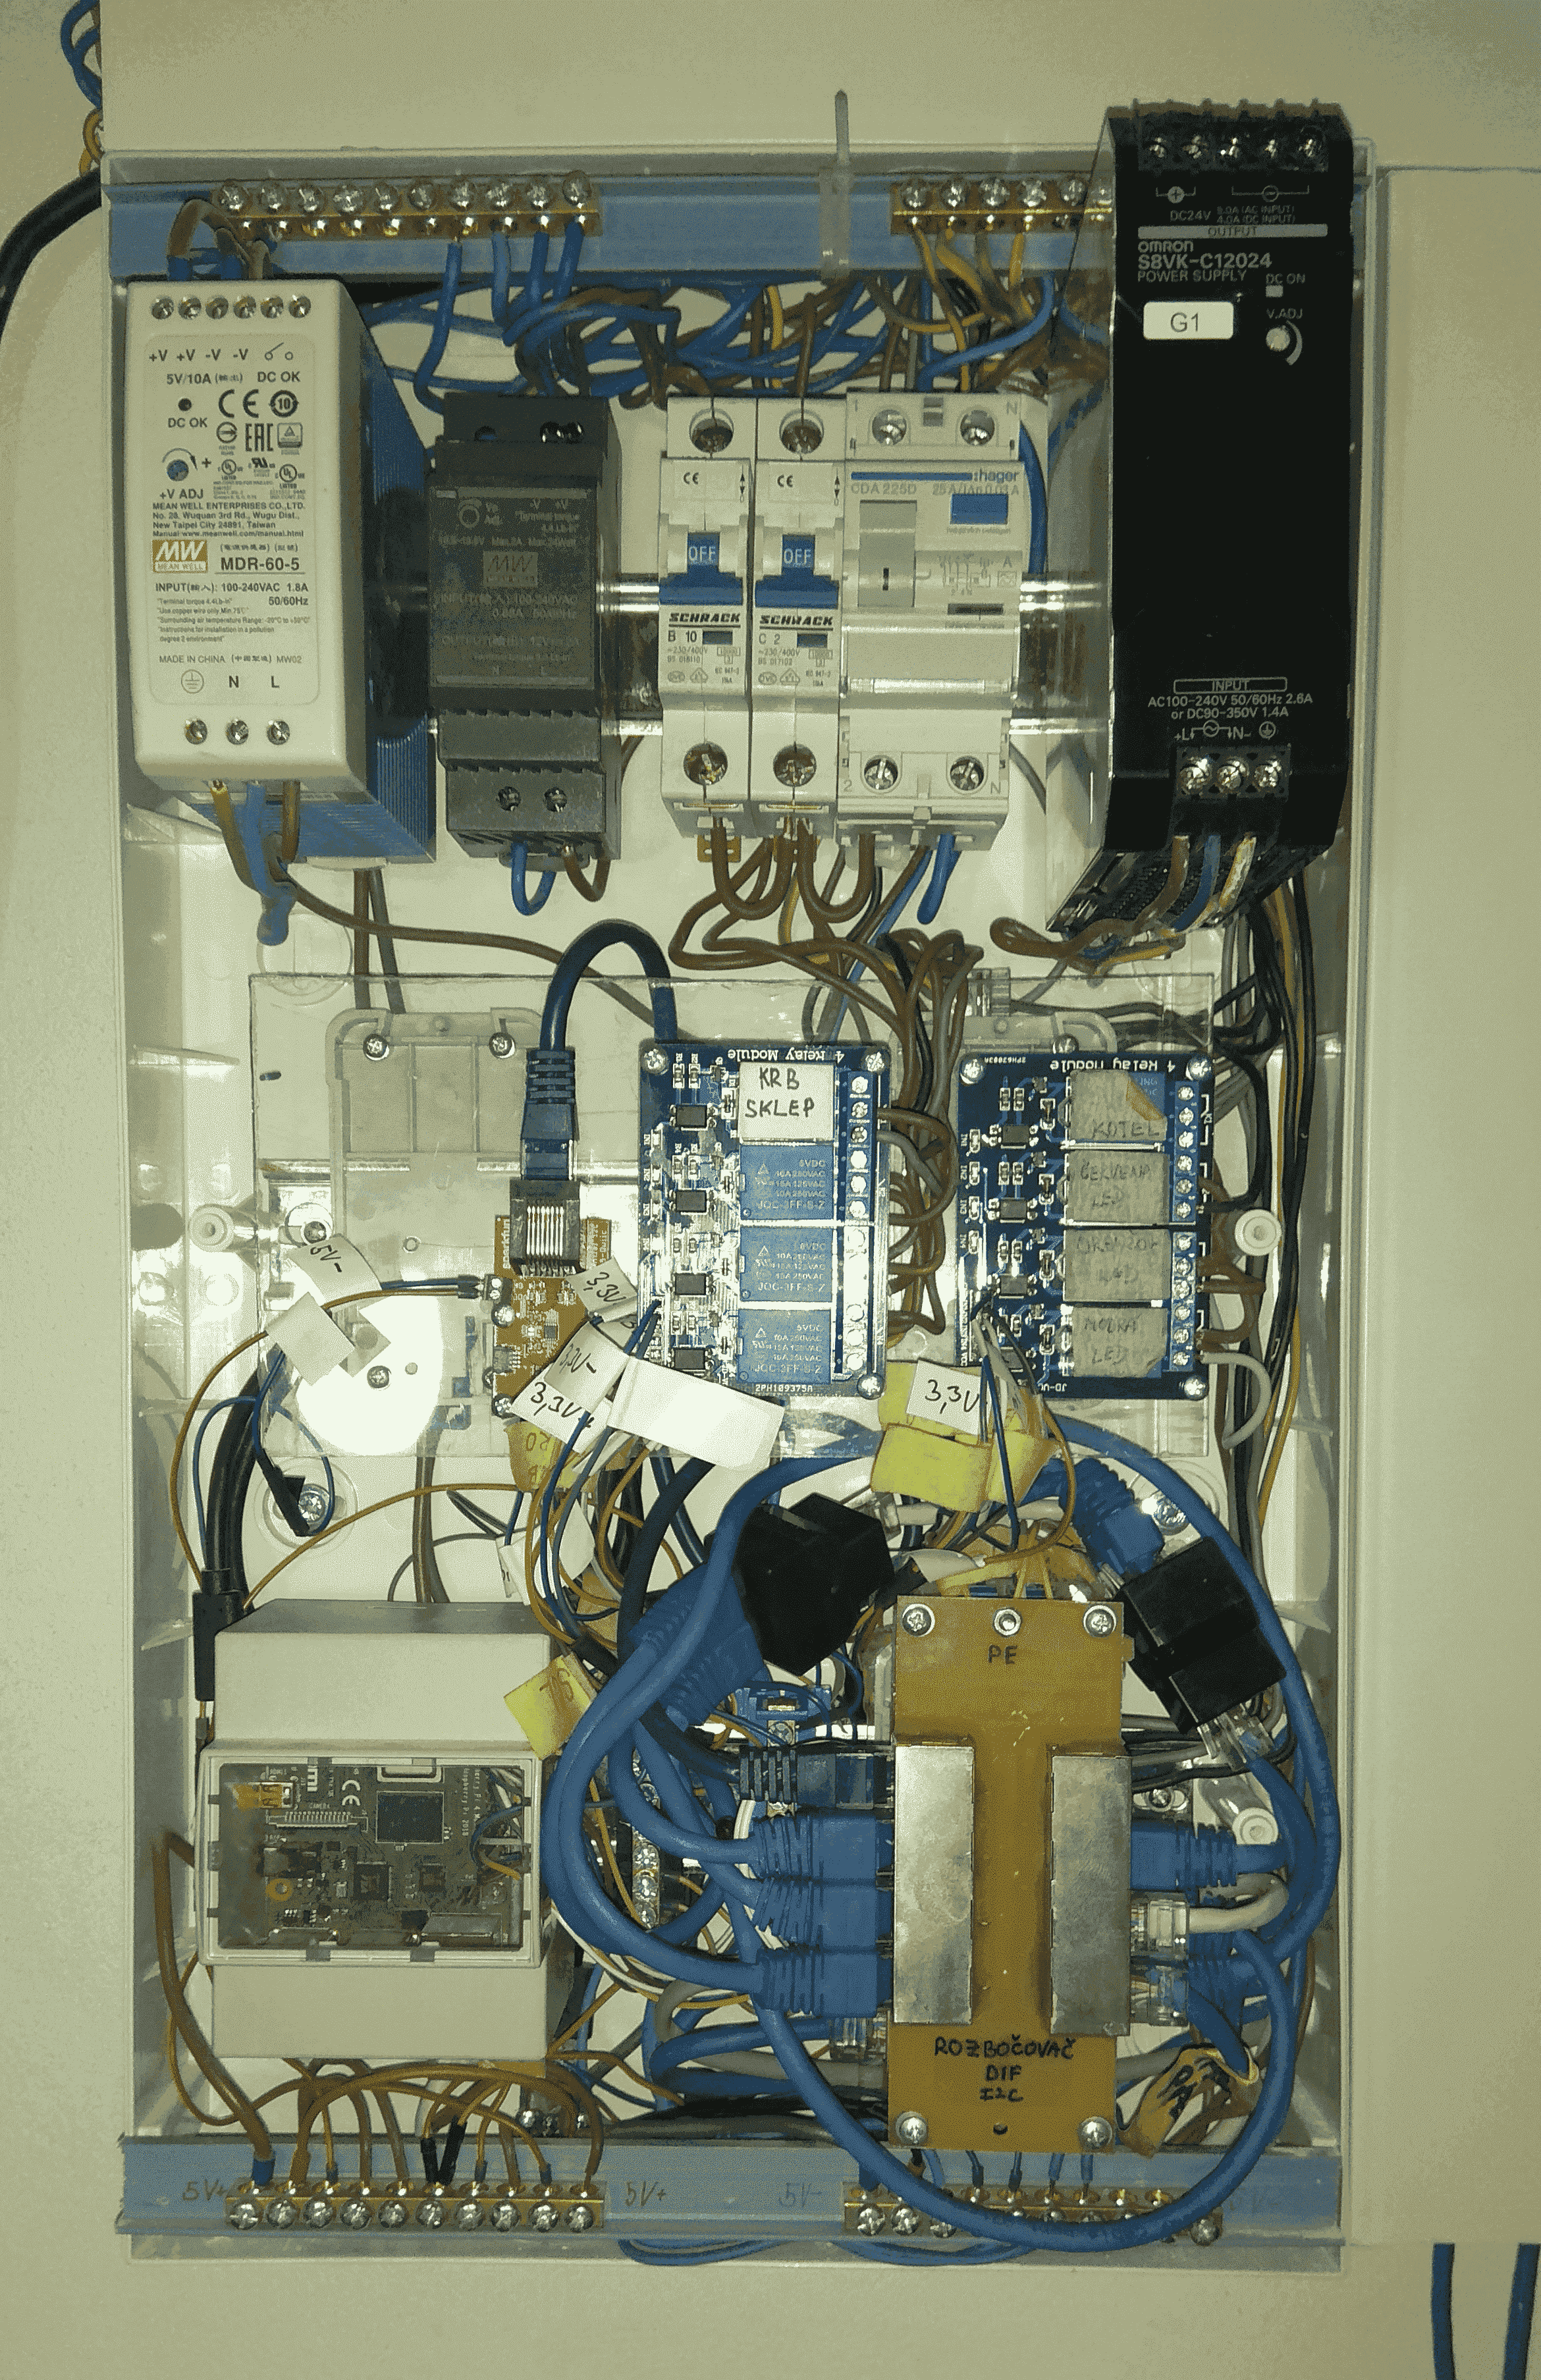
\includegraphics[width=0.99\textwidth]{images/rozvadec-ve-sklepe-s-elektronikou.png}
    \caption[Realizovaný rozvaděč s elektronikou.]{Realizovaný rozvaděč s elektronikou.}
    \label{fig:rozvadec-ve-sklepe-s-elektronikou}
\end{figure}



\chapter{Softwarová část}

\subsection{Nástěnný snímač prostorové teploty}
Pro programování \acrshort{nspt} bylo využito Arduino IDE \cite{arduino-ide}, respektive zápis ve Wiring a C++. Zařízení neustále kontroluje, zda je připojen do sítě (zda je připojen kabel nebo je k dispozici WiFi síť), pokud zjistí, že není. Snaží se připojení obnovit. Uživateli je stav připojení signalizován ikonou v~levém rohu (zelená barva ikony pro úspěšný stav připojení, červená barva signalizuje problém s~připojením). Dále zařízení kontroluje připojení k~MQTT brokeru (Mosquitto broker \cite{mosquitto-broker}), obdobně jako u síťového připojení zařízení se snaží obnovovat automaticky připojení, pokud došlo k výpadku. Stav je opět signalizován pomocí ikony v~levém rohu. Na displeji je červeným písmem zobrazena aktuální naměřená teplota (každých 30 sekund se měří), zeleným písmem je zobrazena požadovaná teplota. Uživatel pravým tlačítkem má možnost inkrementovat teplotu o~+0,5 °C, levé tlačítko dekrementuje o -0,5 °C. Střední tlačítko zatím nemá implementovanou funkci. Plánuje se pro vyvolání menu pro další možnosti nastavení (např. pro nastavení hystereze). Poslední řádek s~bílým písmem slouží pro zobrazení zprávy uživateli, v~současné době je zobrazováno upozornění, zda je potřeba zatopit v krbu. Výše popsané jednotlivé části jsou vidět na obrázku \ref{fig:software-nastenny-snimac-prostorove-teploty-zapnuty-displej}. 

\begin{figure}[H]
\centering
\begin{tikzpicture}[font=\sffamily]
     \node[anchor=south west,inner sep=0] (image) at (0,0) {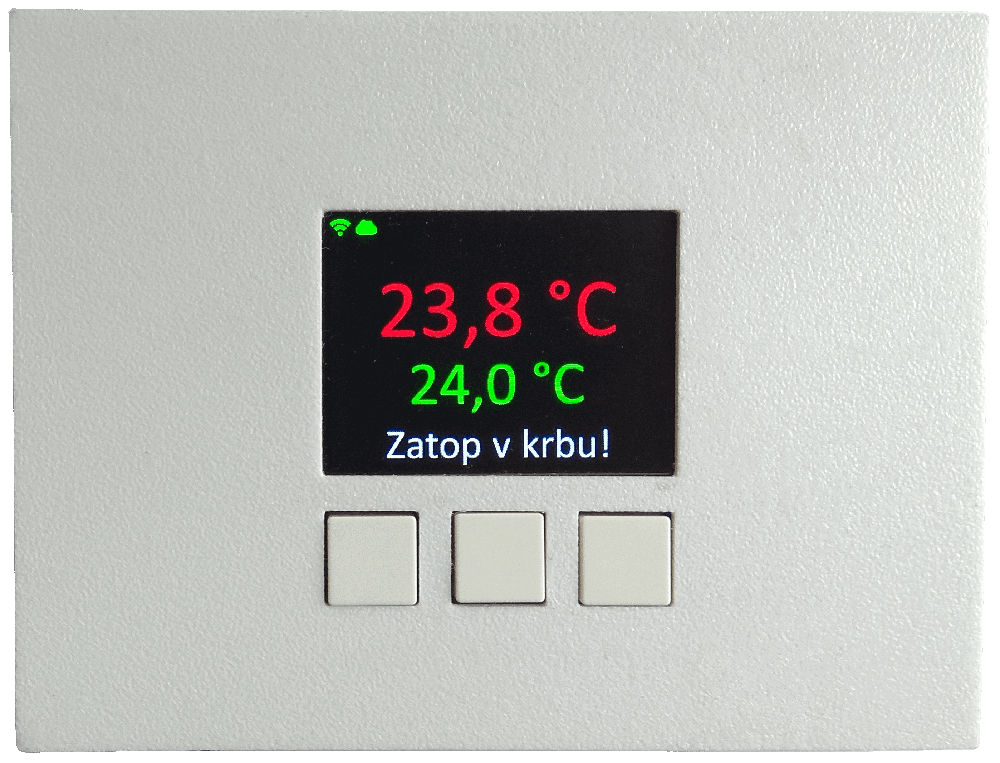
\includegraphics[width=0.9\textwidth]{images/software-ha/nastenny-snimac-prostorove-teploty-zapnuty-displej.png}};
      \begin{scope}[x={(image.south east)},y={(image.north west)}]
     
     %   \draw[help lines,xstep=.1,ystep=.1] (0,0) grid (1,1);
    %    \foreach \x in {0,1,...,9} { \node [anchor=north] at (\x/10,0) {0.\x}; }
       % \foreach \y in {0,1,...,9} { \node [anchor=east] at (0,\y/10) {0.\y}; }
        
          \draw [red,-{Stealth[slant=0]}] (0.2,0.8)--(0.32,0.72);           
          \node[text=red] at (0.2,0.83) {Síťové připojení};
          
          \draw [red,{Stealth[slant=0]}-] (0.38,0.72)--(0.5,0.8);           
          \node[text=red] at (0.5,0.83) {Připojení k MQTT brokeru};
          
          \draw [red,-{Stealth[slant=0]}] (0.25,0.6)--(0.37,0.6);
          \node[text=red] at (0.12,0.6) {Aktuální teplota};
          
          \draw [red,{Stealth[slant=0]}-] (0.6,0.5)--(0.72,0.5);
          \node[text=red] at (0.9,0.5) {Požadovaná teplota};
          
          \draw [red,-{Stealth[slant=0]}] (0.25,0.42)--(0.37,0.42);
          \node[text=red] at (0.12,0.42) {Zpráva uživateli};
          
          \draw [red,-{Stealth[slant=0]}] (0.25,0.26)--(0.37,0.26);
          \node[text=red] at (0.1,0.28) {Dekrementování};
          \node[text=red] at (0.1,0.23) {požadované teploty};
          
          \draw [red,{Stealth[slant=0]}-] (0.62,0.26)--(0.74,0.26);
          \node[text=red] at (0.9,0.28) {Inkrementování};
          \node[text=red] at (0.9,0.23) {požadované teploty};
          
          \draw [red,{Stealth[slant=0]}-] (0.5,0.26)--(0.6,0.1);
          \node[text=red] at (0.65,0.1) {Menu};
        \end{scope}
\end{tikzpicture}
\caption{\acrshort{nspt} s informacemi na displeji.}
\label{fig:software-nastenny-snimac-prostorove-teploty-zapnuty-displej}
\end{figure}

Nastavené QoS pro MQTT přenos zpráv mez WiFi a centrální jednotkou je 2, mezi Ethernetem \acrshort{nspt} a centrální jednotkou je 1. Vzhledem k obsahu zpráv, tedy přenosu především naměřené teploty v 30 sekundovém intervalu, by stačilo QoS 0 (především u kabelového připojení). Zároveň pokud dojde přenastavení teploty v centrálním systému, daná změna se projeví i na příslušném \acrshort{nspt}. Všechna zařízení mají statickou IP adresu. Software pro WiFi a Ethernet \acrshort{nspt} se liší jen v síťové části. Verze ESP-32-WROVER-IE (M213EH2864UH3Q0) má dvě jádra. V současné verzi není striktně vymezeno, které jádro se má používat pro co, dochází k přepínání mezi jádry. Software je udělán s prioritou pro změny uživatele (změna požadované teploty, rozsvícení displeje apod.), tedy aby během změn nedocházelo k prodlevám, které uživatel může registrovat, pokud by se na pozadí něco provádělo (např. odesílání teploty do centrální jednotky, obnova připojení apod.). Pro ověření, že zařízení je připojeno do sítě a komunikuje. Posílá každou minutu aktuální čas do centrální jednotky. Kód pro \acrshort{nspt} je příloze \ref{app:obsah-cd}. Blokové schéma softwaru je příloze \ref{app:software} na obrázku \ref{fig:blokove-schema-nastenny-snimac-prostorove-teploty-ethernet}.


\newpage

\subsection{HA – Typy řízení vytápění}

\label{sec:typy-rizeni-vytapeni}
V rámci řídicího systému existují tyto typy řízení:

\begin{itemize}
  \item Řízení vytápění podle chodbových termostatů.
  \item Řízení vytápění podle nástěnných snímačů prostorové teploty.
  \item Řízení vytápění podle teplotních plánů.
  \item Řízení vytápění podle teplotních plánů s úpravou podle předpovědi počasí.
\end{itemize}

Zjednodušené blokové schéma softwaru HA je příloze \ref{app:software} na obrázku \ref{fig:blokove-schema-ha}, jednotlivé části jsou dále v textu více popsány. Předpokládá se, že centrální \acrshort{zov} je průběžně ohříván během dne pomocí přebytků energie přes výměníky u krbů. Centrální \acrshort{zov} je dohříván pro případné potřeby vytápění. Je kladena priorita na získávání ohřáté otopné vody ze zdroje tepla zmíněná dříve. Uživatelé jsou upozorňováni signalizací na displejích jak u krbů (obrázek \ref{fig:predni-cast-krytu-vika-instalacni-krabice-krb}), tak i na \acrshort{nspt} (obrázek \ref{fig:software-nastenny-snimac-prostorove-teploty-zapnuty-displej}), přímo v řídícím systému (možné i upozornění  na mobil (obrázek \ref{fig:mobil-notifikace}), e-mail) či LED diodami (rozsvícení všech) u~krbů, že je potřeba zatopit v krbech, pokud systém vyhodnotí, že je potřeb vytápět. V případě, že tomu k tomu nedojde využívá se plynový kondenzační kotel, který dohřívá \acrshort{zov} (ten je možný ovládat automaticky).

\begin{figure}[H]
    \centering
    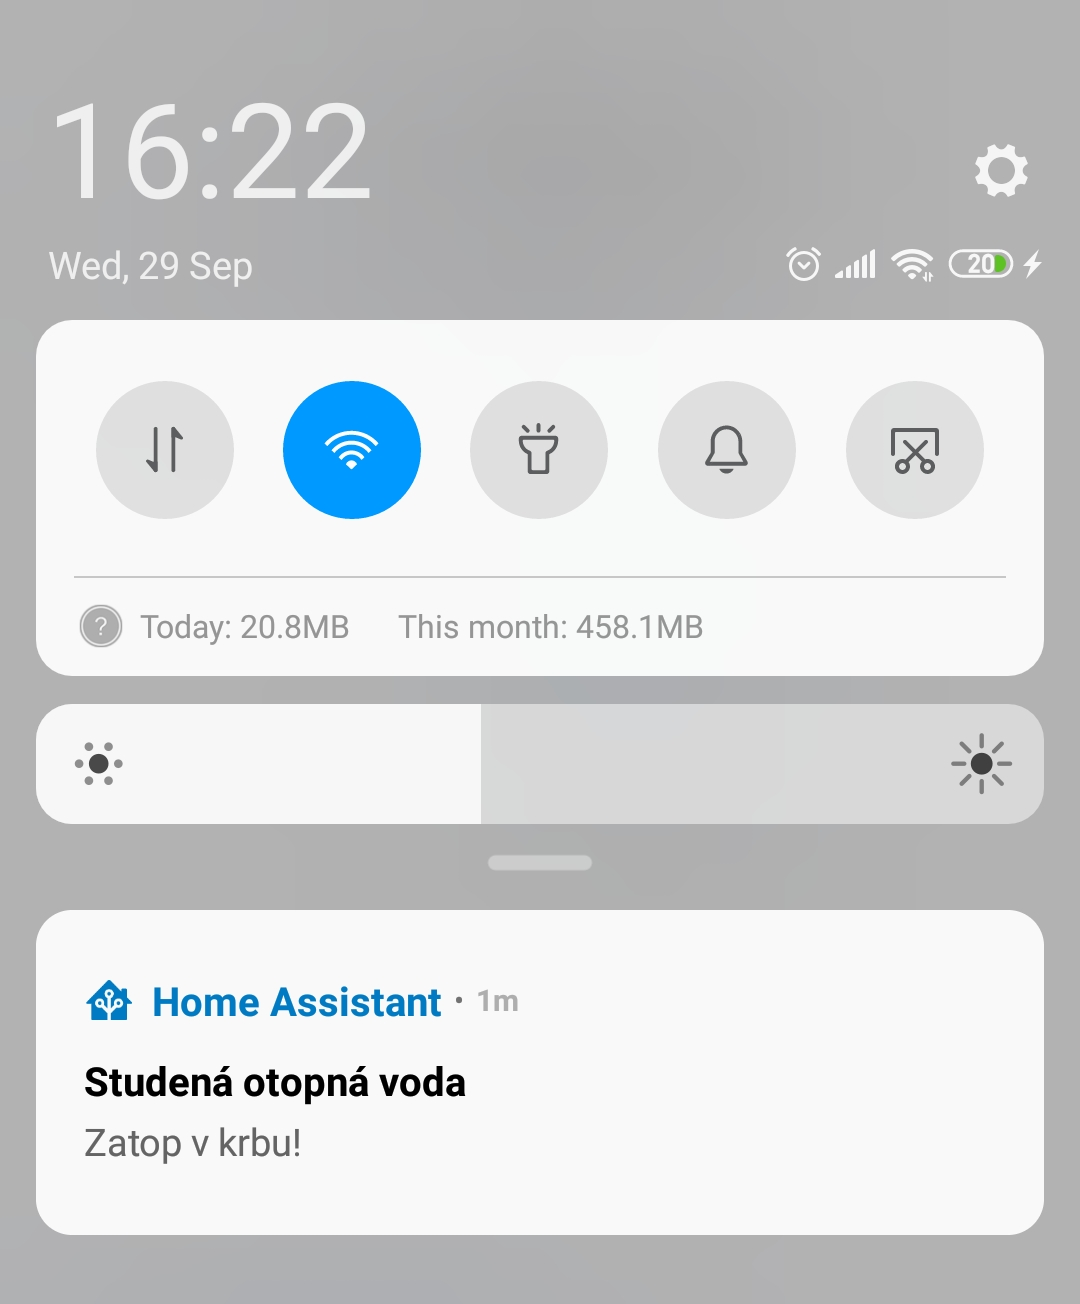
\includegraphics[width=0.4\textwidth]{images/software-ha/mobil-notifikace.png}
    \caption{Upozornění v mobilu.}
    \label{fig:mobil-notifikace}
\end{figure}

Na obrázku \ref{fig:prehled-ha} je rozhraní HA pro nastavení vytápění. V levém menu jsou jednotlivé patra s termostaty a teplotními plány (popsáno níže). V záložce záznamy, historie jsou ukládány do databáze jednotlivé stavy ovládacích prvků a~samotná historie dat, především teplotních senzorů. Dále se zde nachází nastavení uživatelské profilu, tak i celého systému. V horním menu jsou další záložky pro nastavení vytápění, též popsány níže v textu.

\begin{figure}[H]
    \centering
    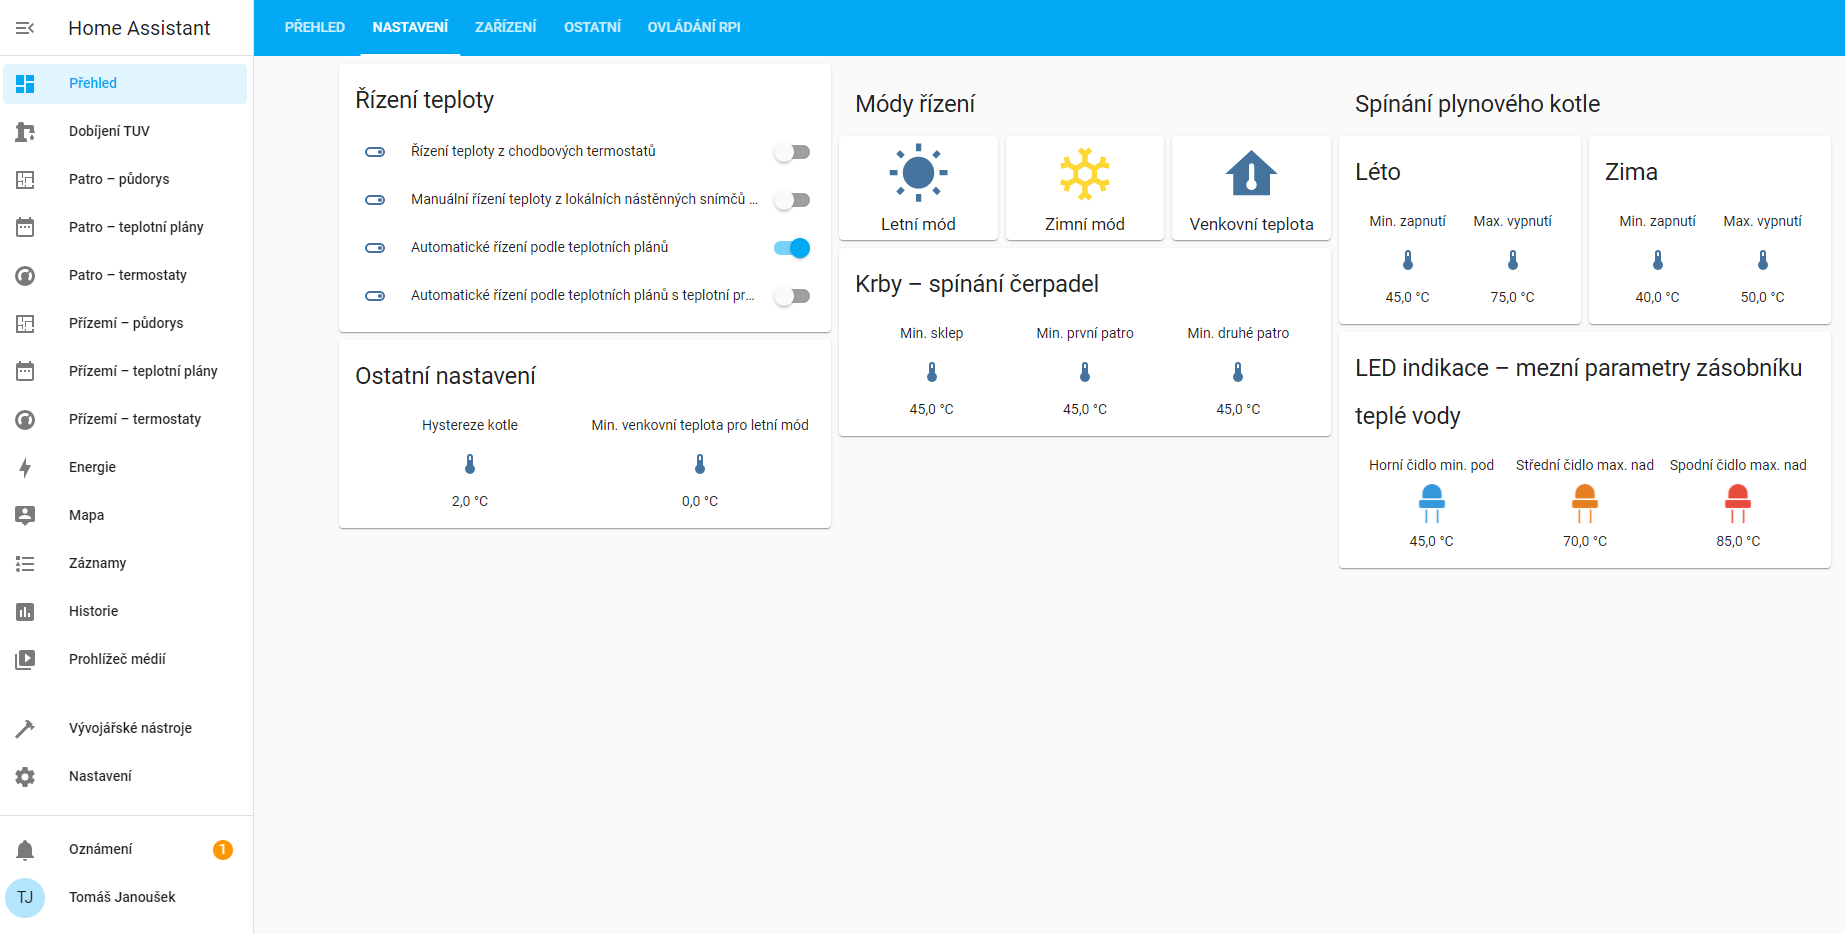
\includegraphics[width=\textwidth]{images/software-ha/prehled-ha.png}
    \caption{Rozhraní HA.}
    \label{fig:prehled-ha}
\end{figure}

V záložce \textbf{přehled} (obrázek \ref{fig:zalozka-prehled}) jsou pro přehlednost zobrazeny aktuální teploty, které se používají pro vyhodnocování v systému HA. V části „jednotlivé teploty“, jsou zde všechny teploty snímané v~\acrshort{zov}, teploty na kouřovodech v přízemí a patře, v neposlední řadě jez zde i~venkovní teplota. V části „porovnání teploty“ jsou zmíněné teploty zobrazeny v jednom grafu.

\begin{figure}[H]
    \centering
    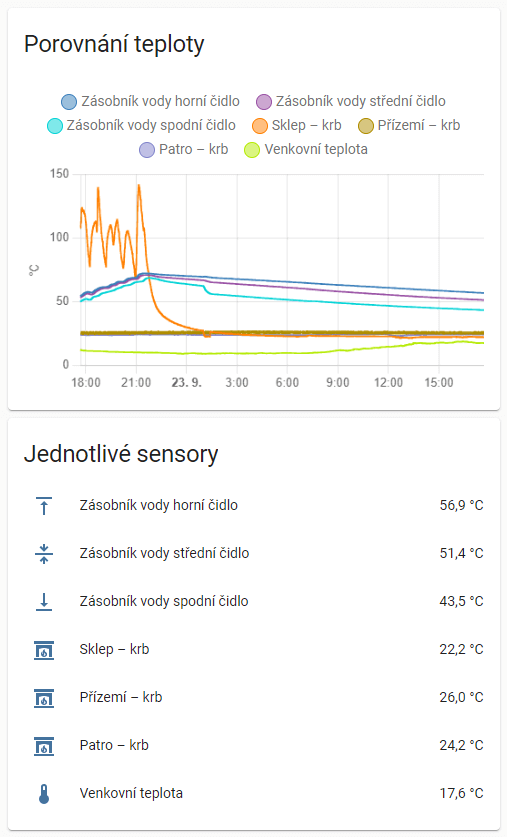
\includegraphics[width=0.6\textwidth]{images/software-ha/zalozka-prehled.png}
    \caption{Záložka přehled v HA.}
    \label{fig:zalozka-prehled}
\end{figure}

V záložce \textbf{nastavení} (obrázek \ref{fig:zalozka-nastaveni}) je možné v části „řízení teploty“ vybrat jeden typ řízení vytápění. Dále v „módy řízení“ je výběr módů a to zimní, letní nebo výběr podle venkovní teploty. Výběr módu má vliv na výběr mezních teplot pro spínání plynového kondenzačního kotle. Dané teplotní meze se dají nastavit v~části „spínání plynového kotle“ (teplotní meze pro léto a zimu). Tyto nastavené meze se berou pro kontrolu s teplotou v horní části \acrshort{zov}. Pokud teplota v~horní části zásobníku je menší než teplota definovaná v části „min. zapnutí“ dojde k~zapnutí kotle pro nahřátí otopné vody, kotel se vypíná při teplotě definované v části „max. vypnutí“. Při porovnávání teplot se též bere v potaz nastavená hystereze v~části „ostatní nastavení“. Při výběru módu podle venkovní teploty dochází k~automatickému výběru letního nebo zimního módu. Teplotní mez pro výběr letního módu (v rámci módu podle venkovní teploty) je definovaná v části „min. venkovní teplota pro letní mód“. Toto spínání kotle nastává v momentě, kdy po upozornění uživatelů nedojde k~zatopení v krbech.


V části nastavení „krby – spínání čerpadel“ se definují minimální hranice teploty, kdy dojde k~sepnutí oběhových čerpadel pro krbové výměníky, tedy při jaké teplotě se má brát v potaz, zda někdo v krbu zatopil a mají se spustit čerpadla pro nahřívání \acrshort{zov}. Toto nastavení je poměrně důležité a kontrola těchto teplot je zcela nezávislá na dalších nastaveních (automatizaci) v systému. V případě zatopení v krbu je potřeba vždy spustit čerpadla, jinak dojde k~přehřátí vody ve výměníku. Pokud nastane přehřátí, tak se aktivuje ochrana přímo u~krbů a dojde ke zvukové signalizaci. Pokud teplota neklesne za určitou dobu, nastane aktivování ochranných ventilů a~vypuštění přehřáté vody.


V části „LED indikace – mezní parametry zásobníku otopné vody“ se definují mezní teploty pro horní, střední a spodní část \acrshort{zov}. Tato signalizace se zejména týká krbů, aby uživatel věděl, zda může topit, a jak je moc zásobník nahřátý. U modré LED se definuje mezní minimální teplota, kterou by zásobníku v horní části měl mít (povolení pro topení). U oranžové LED se definuje mezní maximální teplota, kdy ve střední části zásobníku dochází k dostatečnému nahřátí otopné vody (oznámení, že za chvilku by se mělo přestat topit). U červené LED se definuje mezní maximální teplota, kdy ve spodní části zásobníku je plně ohřátá(okamžitě přestat topit.). Aktivace červené LED předchází v dostatečném předstihu před aktivováním ochrany u~krbů pro přehřátí otopné vody, popsáno v předchozím odstavci.

\begin{figure}[H]
    \centering
    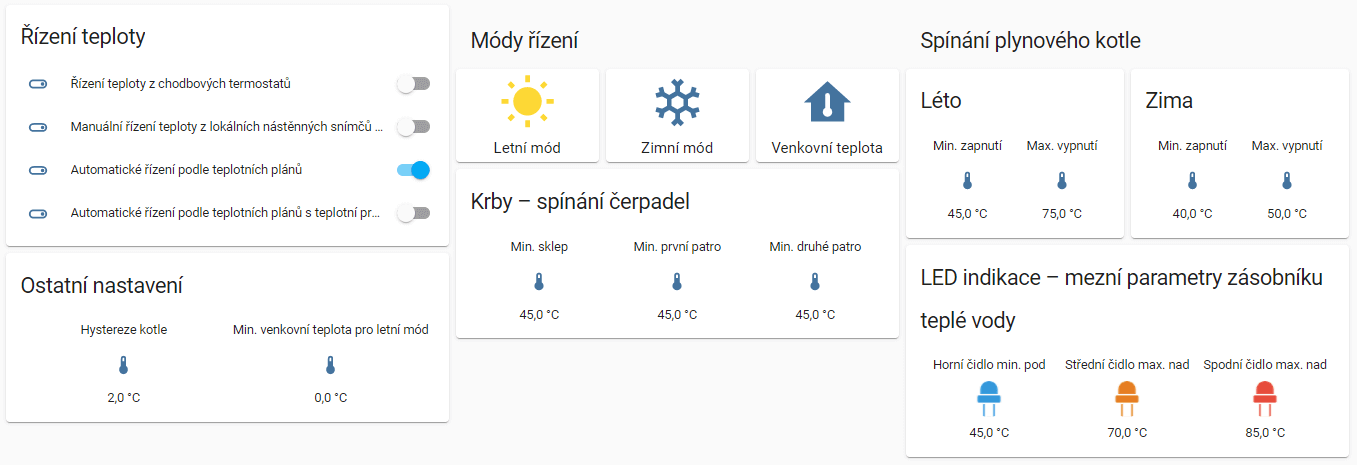
\includegraphics[width=\textwidth]{images/software-ha/zalozka-nastaveni.png}
    \caption{Záložka nastavení v HA.}
    \label{fig:zalozka-nastaveni}
\end{figure}

V záložce \textbf{zařízení} (obrázek \ref{fig:zalozka-zarizeni}) se zobrazují jednotlivá ovládána (zapnuto/vypnuto) zařízení otopné soustavy, tedy plynový kondenzační kotel, čerpadla pro krby s výměníkem, čerpadla pro podlahové vytápění a zapnutí signalizačních LED u krbů. Je možné samotnou automatizaci respektive ovládání zmíněných zařízení řídit podle vlastního uvážení, proto slouží přepínač „manuální ovládání zařízení“. Zde si pak uživatel může libovolně jednotlivá zařízení ovládat bez ohledu na nastavenou automatizaci.

V části „termostaty chodby – požadavek topení“, zde se zobrazuje zda dochází k vytápění v~přízemí či patře na základě nastavení chodbových termostatů.

V části „patro/přízemí – otopné okruhy (ventily)“ se zobrazuje pro přehlednost stav každého ventilu pro daný otopný okruh.

\begin{figure}[H]
    \centering
    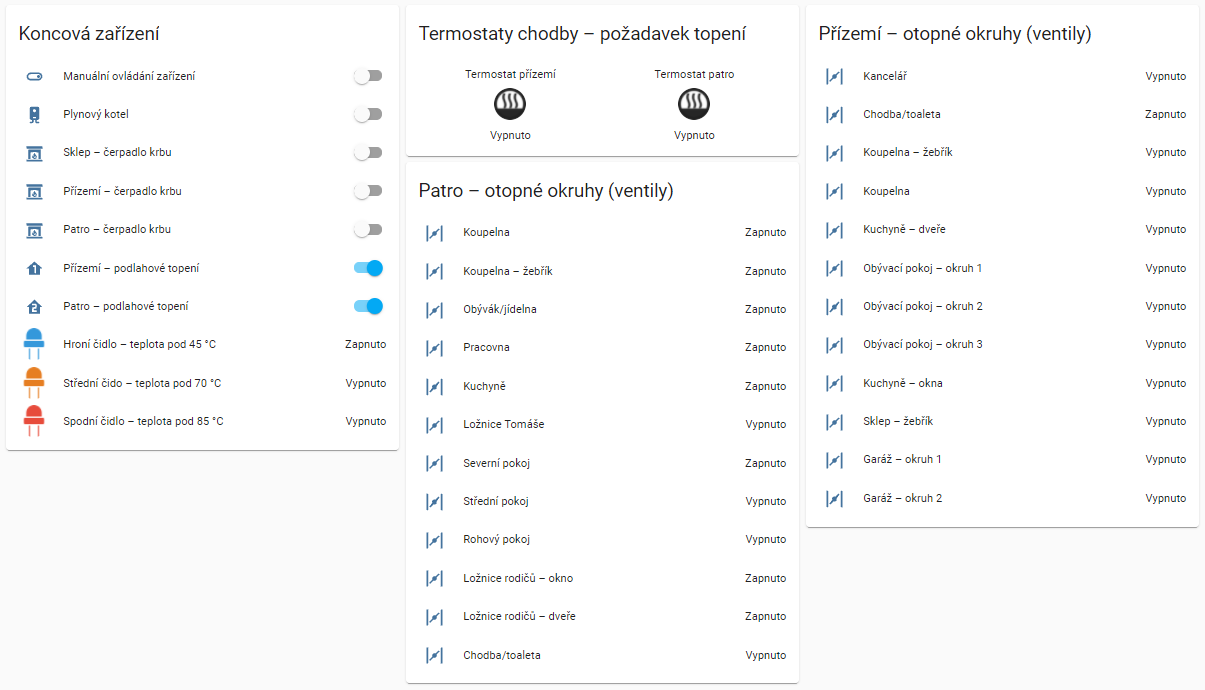
\includegraphics[width=\textwidth]{images/software-ha/zalozka-zarizeni.png}
    \caption{Záložka zařízení v HA.}
    \label{fig:zalozka-zarizeni}
\end{figure}

V záložce \textbf{ostatní} je v části „ovládání čerpadel – vodní kámen“ (obrázek \ref{fig:zalozka-ostatni}) slouží ke spínání čerpadel pro ochranu před zatuhnutím lopatek. Vzhledem k místní dosti tvrdé vodě, došlo při netopení, tedy při nevyužívání daných čerpadel k zatuhnutí lopatek v důsledku nánosu vodního kamene. Proto se zde nachází nastavení, kde si uživatel může pro konkrétní den, hodinu a~definovanou délku nastavit spínání čerpadel pro odstranění nánosu na lopatách. Ideální volbou je otopnou vodu zbavit minerálů nebo vyměnit za destilovanou vodu, nicméně k některým méně kvalitnějším provedením spojům trubek otopné soustavy, by docházelo k průsaku otopné vody. Proto je otopná voda z řádu s vyšším podílem minerálů jedním z řešení, jak docílit zaslepení průsaku především vápníkem bez nutnosti, alespoň prozatím, spoje opravovat.

\begin{figure}[H]
    \centering
    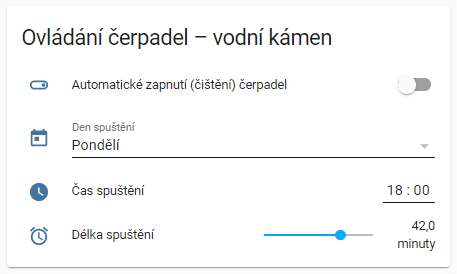
\includegraphics[width=0.7\textwidth]{images/software-ha/zalozka-ostatni.png}
    \caption{Záložka ostatní v HA.}
    \label{fig:zalozka-ostatni}
\end{figure}


\subsubsection{Řízení vytápění podle chodbových termostatů}
V přízemí a v patře je na chodbě umístěn jeden chodbový termostat popsaný v~části \ref{sec:digitalni-chodbove-termostaty}. Tento termostat na základě lokálního nastavení (není součástí řídicího systému) spínání/rozpínání výstupní relé při požadavku na vytápění. Tento požadavek se následně vyhodnotí v centrálním systému (popsáno v části \ref{sec:typy-rizeni-vytapeni} v části zařízení) a dojde k sepnutí nebo rozepnutí daného chodbového oběhového čerpadlo pro podlahové vytápění a~otevření všech okruhů podlahové vytápění. Dochází tedy k řízení vytápění všech místností na patře podle jednoho centrálního termostatu. 

\subsubsection{Řízení vytápění podle nástěnných snímačů prostorové teploty}
\label{sec:rizeni-vytapeni-podle-nastennych-snimacu-prostorove-teploty}
Podle aktuální teploty naměřenou z každé místnosti je ovládán daný otopný okruh pro vytápění. Na základě požadované teploty, kterou je možné zadat přímo v systému HA (viz obrázek \ref{fig:lokalni-termostat-ha}) nebo je možné teplotu nastavit přímo v~místnosti pomocí tlačítek na \acrshort{nspt}, tím dojde k přenesené požadované teploty do systému a zobrazení na daném termostatu, nastavení funguje i opačně. Řízení vytápění místnosti je dáno hysterezí 0,5~°C. Regulace vytápění tedy reaguje na aktuální naměřenou teplotu.

\begin{figure}[H]
    \centering
    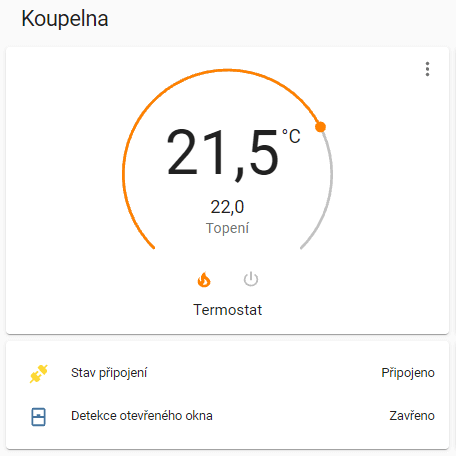
\includegraphics[width=0.6\textwidth]{images/software-ha/lokalni-termostat-ha.png}
    \caption{Nástěnný snímač prostorové teploty v HA.}
    \label{fig:lokalni-termostat-ha}
\end{figure}

Lokální termostaty jsou roztříděny do skupiny podle daného patra, kde se nalézají, tedy termostaty pro přízemí a patro (příklad sdružení termostatů pro patro je na obrázku \ref{fig:prehled-lokalnich-termostaty-patro}, obdobně vypadá i pro přízemí).

\begin{figure}[H]
    \centering
    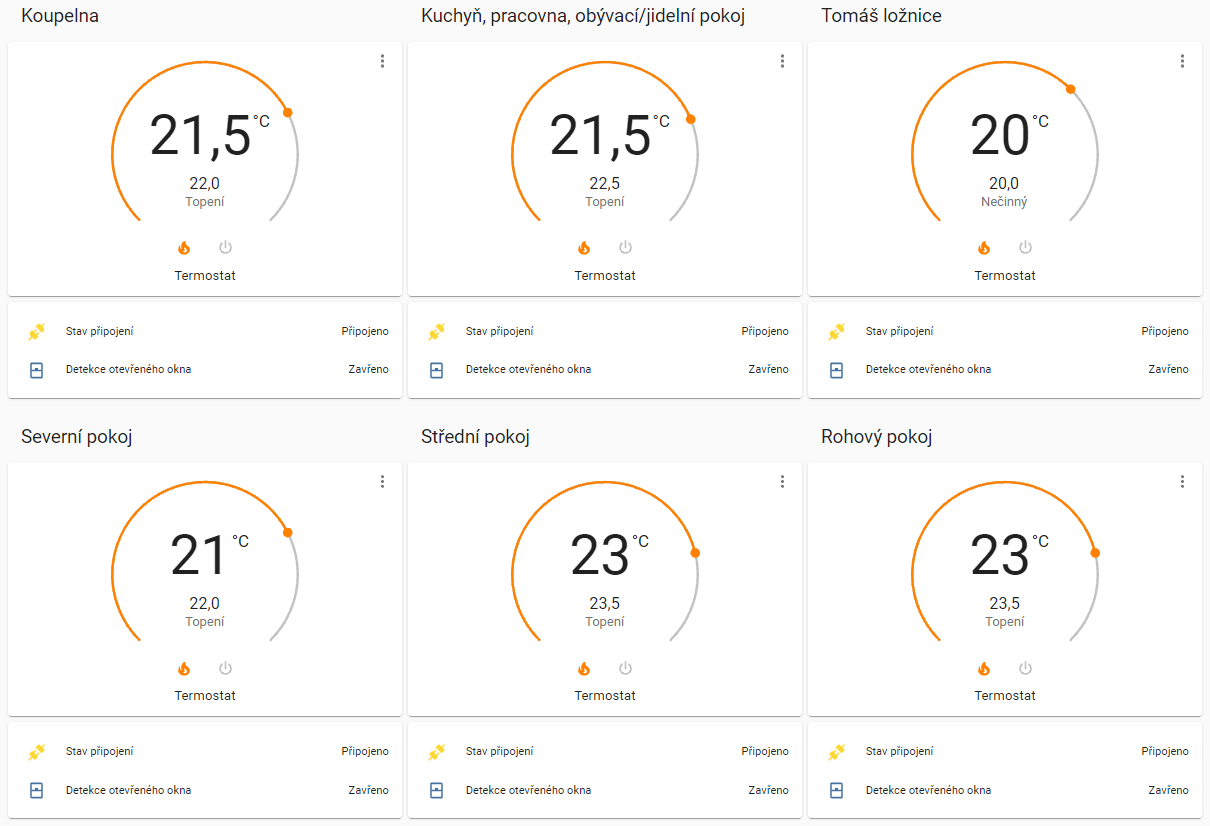
\includegraphics[width=\textwidth]{images/software-ha/prehled-lokalnich-termostaty-patro.png}
    \caption{Skupina nástěnných snímačů prostorové teploty v HA pro patro.}
    \label{fig:prehled-lokalnich-termostaty-patro}
\end{figure}

Každý termostat má dále zobrazení, zda je koncový \acrshort{nspt} připojen k~centrální jednotce.  Ověření probíhá na základě posílaní aktuálního času, který se porovnává s časem v~centrální jednotce zpožděný o~minutu. Pokud zařízení neposílá aktuální čas, dojde ke zpoždění a~zařízení se vyhodnotí jako nepřipojené. V takovém případě dojde k zastavení vytápění pro danou místnost, dokud není spojení obnoveno. Dále je zde detekce otevřeného okna, tato funkce je více popsána v části \ref{sec:detekce-otevreneho-okna}. V~případě otevřeného okna je uživatel informován pomocí upozornění. 



\subsubsection{Řízení vytápění podle teplotních plánů} 
\label{sec:rizeni-vytapeni-podle-teplotnich-planu}
Další možností řízení vytápění jednotlivých místností je podle nadefinovaných časových plánů. Uživatel má možnost si pro každou místnost v rámci 24 hodin nadefinovat časové úseky s danou požadovanou teplotou. Takto nastavené časové plány se průběžně kontrolují systémem a nastavuje aktuálně požadovanou teplotu do lokálních \acrshort{nspt}. Tato teplota se objeví i~na termostatu v HA (viz obrázek \ref{fig:lokalni-termostat-ha}). Následně dochází k regulaci vytápění podle popisu v části \ref{sec:rizeni-vytapeni-podle-nastennych-snimacu-prostorove-teploty}. Rozhraní pro nastavení časových úseků je na obrázku \ref{fig:teplotni-plan-ha}. Uživatel si může jednotlivé úseky přidávat nebo odebírat (min. počet časových úseků jsou dva). Uživatel má na výběr, zda se časové úseky aplikují na všechny v dny v týdnu nebo jen pracovní dny, víkend či výběr konkrétních dnů v týdnu. Dále je možné nadefinovat, zda se pro daný úsek má vytápět nebo naopak nemá.

\begin{figure}[H]
    \centering
    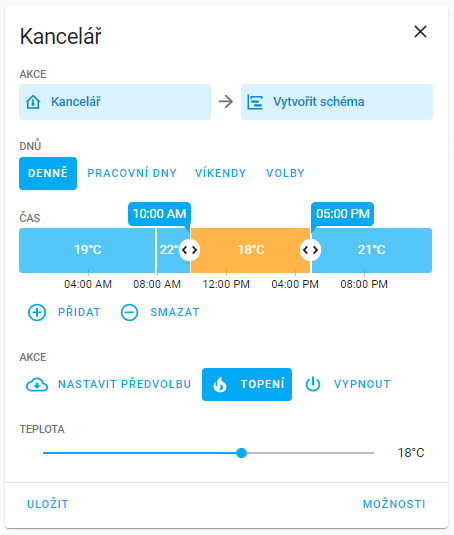
\includegraphics[width=0.8\textwidth]{images/software-ha/teplotni-plan-ha.png}
    \caption{Rozhraní pro nastavení teplotního plánu.}
    \label{fig:teplotni-plan-ha}
\end{figure}

Pro každou místnost je možné nadefinovat libovolný počet časových plánů. Přehled jednotlivých plánů je zobrazen pod každým dnem, viz obrázek \ref{fig:teplotni-plany-ha}. Jednotlivé plány je také možné pozastavit pomocí posuvného tlačítka vpravo. Celkový přehled teplotních plánů všech místností pro patro je vidět na obrázku \ref{fig:teplotni-plany-prehled-ha}, obdobně vypadá i pro přízemí.

\begin{figure}[H]
    \centering
    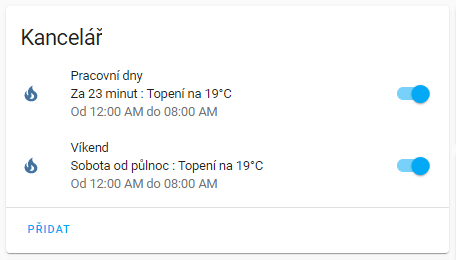
\includegraphics[width=0.7\textwidth]{images/software-ha/teplotni-plany-ha.png}
    \caption{Jednotlivé plány pro danou místnost.}
    \label{fig:teplotni-plany-ha}
\end{figure}


\begin{figure}[H]
    \centering
    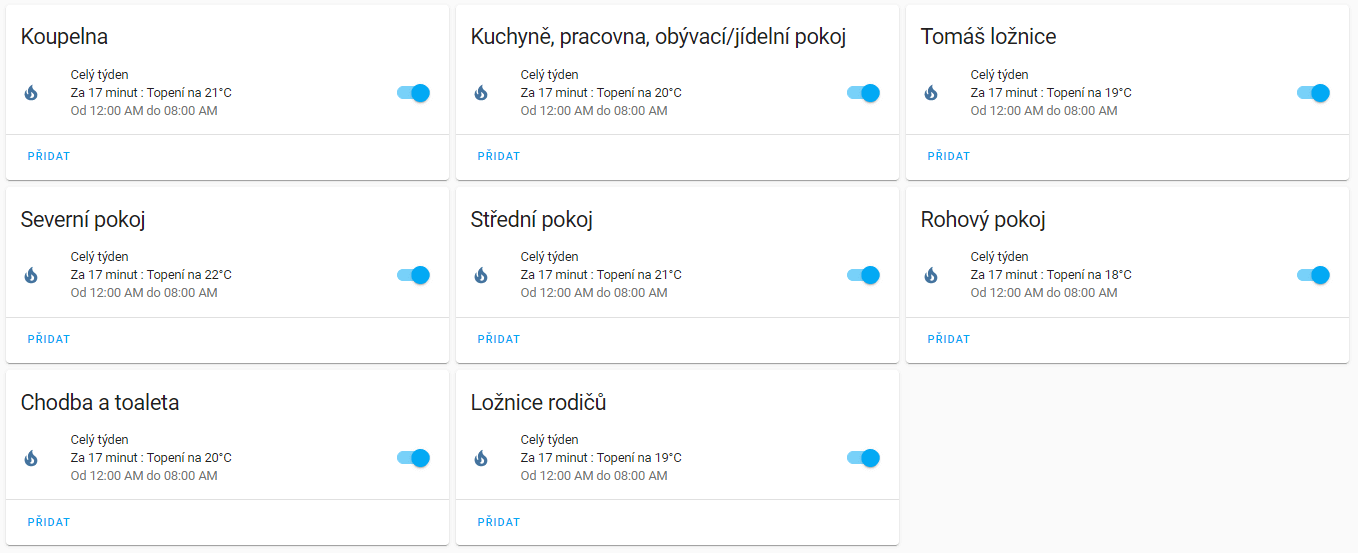
\includegraphics[width=\textwidth]{images/software-ha/teplotni-plany-prehled-ha.png}
    \caption{Přehled teplotních plánů pro patro.}
    \label{fig:teplotni-plany-prehled-ha}
\end{figure}

\subsubsection{Řízení vytápění podle teplotních plánů s úpravou podle předpovědi počasí.} 
\label{sec:rizeni-vytapeni-podle-teplotnich-planu-s-upravou-podle-predpovedi-pocasi}
Řízení vytápění podle teplotních plánů s úpravou podle předpovědi počasí probíhá obdobně, jako v případě popisu v části \ref{sec:rizeni-vytapeni-podle-teplotnich-planu}. Rozdílem je, že jednou týdně si systém „osahá“ místnost a určí si převodní charakteristiku, podle které  upravuje teplotní plány (více v části \ref{sec:teplotni-predikce}).

\subsection{Dobíjení TUV}
Obdobně jako pro vytápění pomocí teplotních plánů je řešeno dobíjení TUV. Pro dobíjení TUV existuje jeden teplotní plán, dochází k porovnání nastavené teploty s aktuální teplotou v horní části \acrshort{zov}. Pokud je teplota nízká, systém upozorní uživatele (zmíněné v části \ref{sec:typy-rizeni-vytapeni}), aby zatopili v~krbu. Pokud tak neučiní do určité doby, dojde k automatickému zapnutí plynového kotle a~nahřátí vrchní části \acrshort{zov}. 

\subsection{Schopnosti automatizovaného provozu}
\subsubsection{Detekce otevřeného okna}
\label{sec:detekce-otevreneho-okna}
Pro detekci otevřeného okna se vyhodnocuje gradient teploty. Tato funkce je již v HA integrovaná pomocí platformy Trend, bylo nutné definovat samotný gradient, tedy číslo pro minimální změnu teploty za určité časové období, kdy dojde k detekci otevřeného okna (poklesu teploty v místnosti). Detekce není vždy přesná, optimální je použít samotný senzor pro detekci otevřeného okna (magnetický senzor), nicméně tento senzor je nutné montovat na každé okno (cenové prodražení, nutné další kabely).

\subsubsection{Teplotní predikce}
\label{sec:teplotni-predikce}
Softwarový návrh pro teplotní predikci vychází z \cite{teplotni-predikce}. Na základě historický dat (7 dní) systém automaticky provádí pro každou místnost zvlášť takzvané „teplotní osahání místnosti“ spočívající v matematické metodě lineární regrese (aproximace naměřených hodnot metodou nejmenších čtverců). Podle vnitřní, venkovní teploty a doby zapnutí jednotlivých termoelektrických pohonů (doby vytápění) pro danou místnost se získá převodní charakteristika, závislost doby vytápění na rozdílu vnitřní a venkovní teploty. Tato jednoduchá aproximace se využívá pro definované teplotní plány (část \ref{sec:rizeni-vytapeni-podle-teplotnich-planu-s-upravou-podle-predpovedi-pocasi} Řízení vytápění podle teplotních plánů s úpravou podle předpovědi počasí). Z jednotlivých teplotních úseků se vezme jejich začátek a pro danou hodinu se vybere teplota z předpovědi počasí. Tato teplota se následně využívá v~dané lineární aproximace a určí se v minutách, o kolik je nutné úsek posunout. Tím se zajistí, že v požadovaný čas bude v~místnosti požadovaná teplota. Každý týden se udělá nová lineární aproximace pro danou místnost.

\subsection{Vizualizace aktuálních stavů}
Pro každé patro je v levém menu půdorys daného patra. V každém půdorysu pro každou místnost se zobrazuje aktuální a požadováná teplota, zda se v dané místnosti topí, detekce otevřeného okna a v neposlední řadě, zda se topí v krbu. Půdorys pro patro je na obrázku \ref{fig:vizualizace-hodnot-patro-pudorys}. Jednotlivé stavy se dají rozkliknout a zobrazit jejich historii, případně změnit požadovanou teplotu. Půdorys v~případě potřeby je snadno modifikovatelný.

\begin{figure}[H]
    \centering
    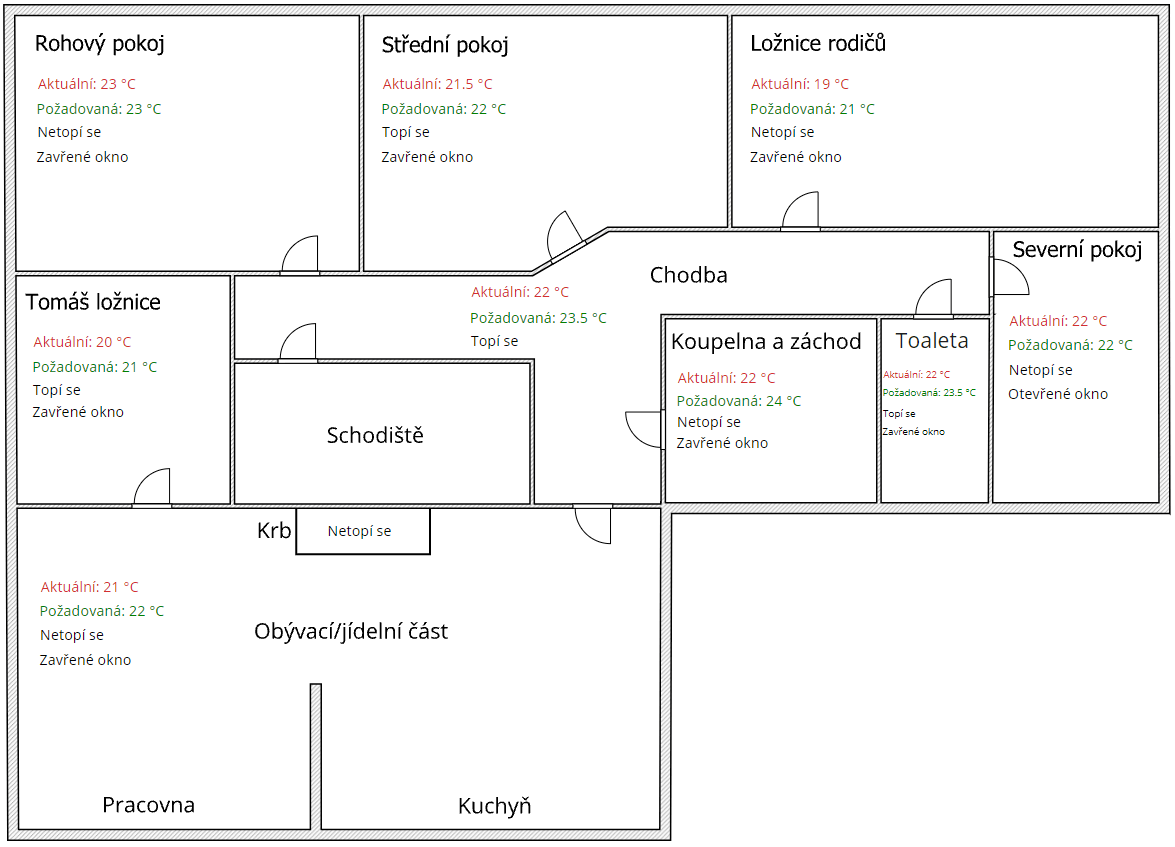
\includegraphics[width=\textwidth]{images/software-ha/vizualizace-hodnot-patro-pudorys.png}
    \caption{Vizualizace aktuálních stavů pro patro.}
    \label{fig:vizualizace-hodnot-patro-pudorys}
\end{figure}


\section{Zápis automatizace}
Primárně pro zápis automatizace se využívá \acrshort{yaml} (\textit{\acrlong{yaml}}). Dále mezivrstvu mezi systémem HA a využití vlastních Python knihoven s návazností na objekty v HA využívám AppDaemon (externí modul). Appdaemon využívám pro obsluhu LCD displejů, zónových regulátorů, teplotních senzorů, pro čtení hodnoty z chodbových termostatů a pro předpřípravu dat pro „osahání teploty v místnosti“.. 

\subsection{Přidání grafických komponent}
Obecně u komponent jsou povinné a nepovinné položky (mají svojí výchozí hodnotu). Mezi ty povinné tedy patří výběr komponenty, kterou chceme (input$\_$text, input$\_$select, input$\_$boolean apod.), dále název komponenty (lze volitelně zvolit), přes který dále s komponentou pracujeme například v~automatizaci. O tom, co je a není povinné, se dozvíme v dokumentaci každé komponenty na webu HA.

Příklad přidání komponenty input$\_$text. Input$\_$text nám říká jakou komponentu chceme, dále následuje název této komponenty, přes tento název dále v programu přistupujme k této komponentě. Dále je zde řádek s name,
jedná se o název, který se zobrazí uživateli. Initial je počáteční text, který se zobrazí. Min definuje minimální délku řetězce. Max definuje maximální délku řetězce. Pattern validuje vstup, jaké znaky jsou povoleny.

\begin{lstlisting}
input_text:
	name_input_text:
		name: "Zobrazený název v gui"
		initial: "Inicializační text"
		min: 8
		max: 40
		pattern: "[a-fA-F0-9]*"
\end{lstlisting}

\subsection{Konfigurace automatizace}

Automatizace se skládá ze tří základních částí:

\begin{itemize}
\item Spouštěč automatizace, spuštění může být například, že někdo přijde
domů, je zapnuto tlačítko, zajde Slunce, spouštěč může být konkrétní
čas, datum apod.
\item Podmínka omezující spouštěč. Může se jednat třeba o časovou podmínku, že aktuální čas se musí rovnat požadovanému. Zadaný vstup musí
být větší než požadované číslo apod.
\item Akce vykonaná při splnění všech podmínek. Akcí může být zapnutí
zařízení, zobrazení upozornění, poslání sms apod.
\end{itemize}

Příklad automatizace:

\begin{lstlisting}
(spouštěč) Když Pavel dorazí domů
(podmínka) a Slunce zapadlo
(akce) 	   Rozsviť světla v obývacím pokoji
\end{lstlisting}

%\section{Výměna dat mezi centrální jednotkou a~nástěnnými snímači prostorové teploty}
%Jak již bylo řečeno v části \ref{sec:mqtt-protokol} pro výměnu dat mezi centrální jednotkou a~nástěnnými snímači prostorové teploty využívám MQTT protokol. Nástěnný snímač prostorové teploty posílá do centrální jednotky aktuálně naměřenou teplotu pro danou místnost, případně pokud uživatel změní požadovanou teplotu, tato změna se projeví i v systému. Naopak pokud v systému dojde ke změně požadované teploty, tato teplota se projeví i v  nástěnném snímači prostorové teploty pro danou místnost. Dále pokud je požadavek, aby uživatelé začali topit v krbech (viz část \ref{sec:typy-rizeni-vytapeni}) a nedojde k tomu stavu za určitou dobu, jsou uživatelé informování zprávou na displeji. 

%\section{Síťová část}
%Všechny nástěnné snímače prostorové teploty mají přidělenou statickou IP adresu. Též mají definovanou vlastní MAC adresu. Je možné využít i DHCP, ale pro stálost zařízení jsem využil statické IP adresy. Do rozhraní HA, lze vstoupit přes webový prohlížeč s adresou http:$\slash \slash$homeassistant:8123 nebo http:$\slash \slash$ip$\_$adresa$\_$rpi:8123. Lze pro přístup využít i mobilní telefon s Android nebo iOS systémem, kterou lze oficiálně stáhnout z daných obchodů s~aplikacemi. Celé rozhraní je velmi responzivní, viz obrázek \ref{fig:mobilni-aplikace} pro systém Android.

%\begin{figure}[H]
%    \centering
%    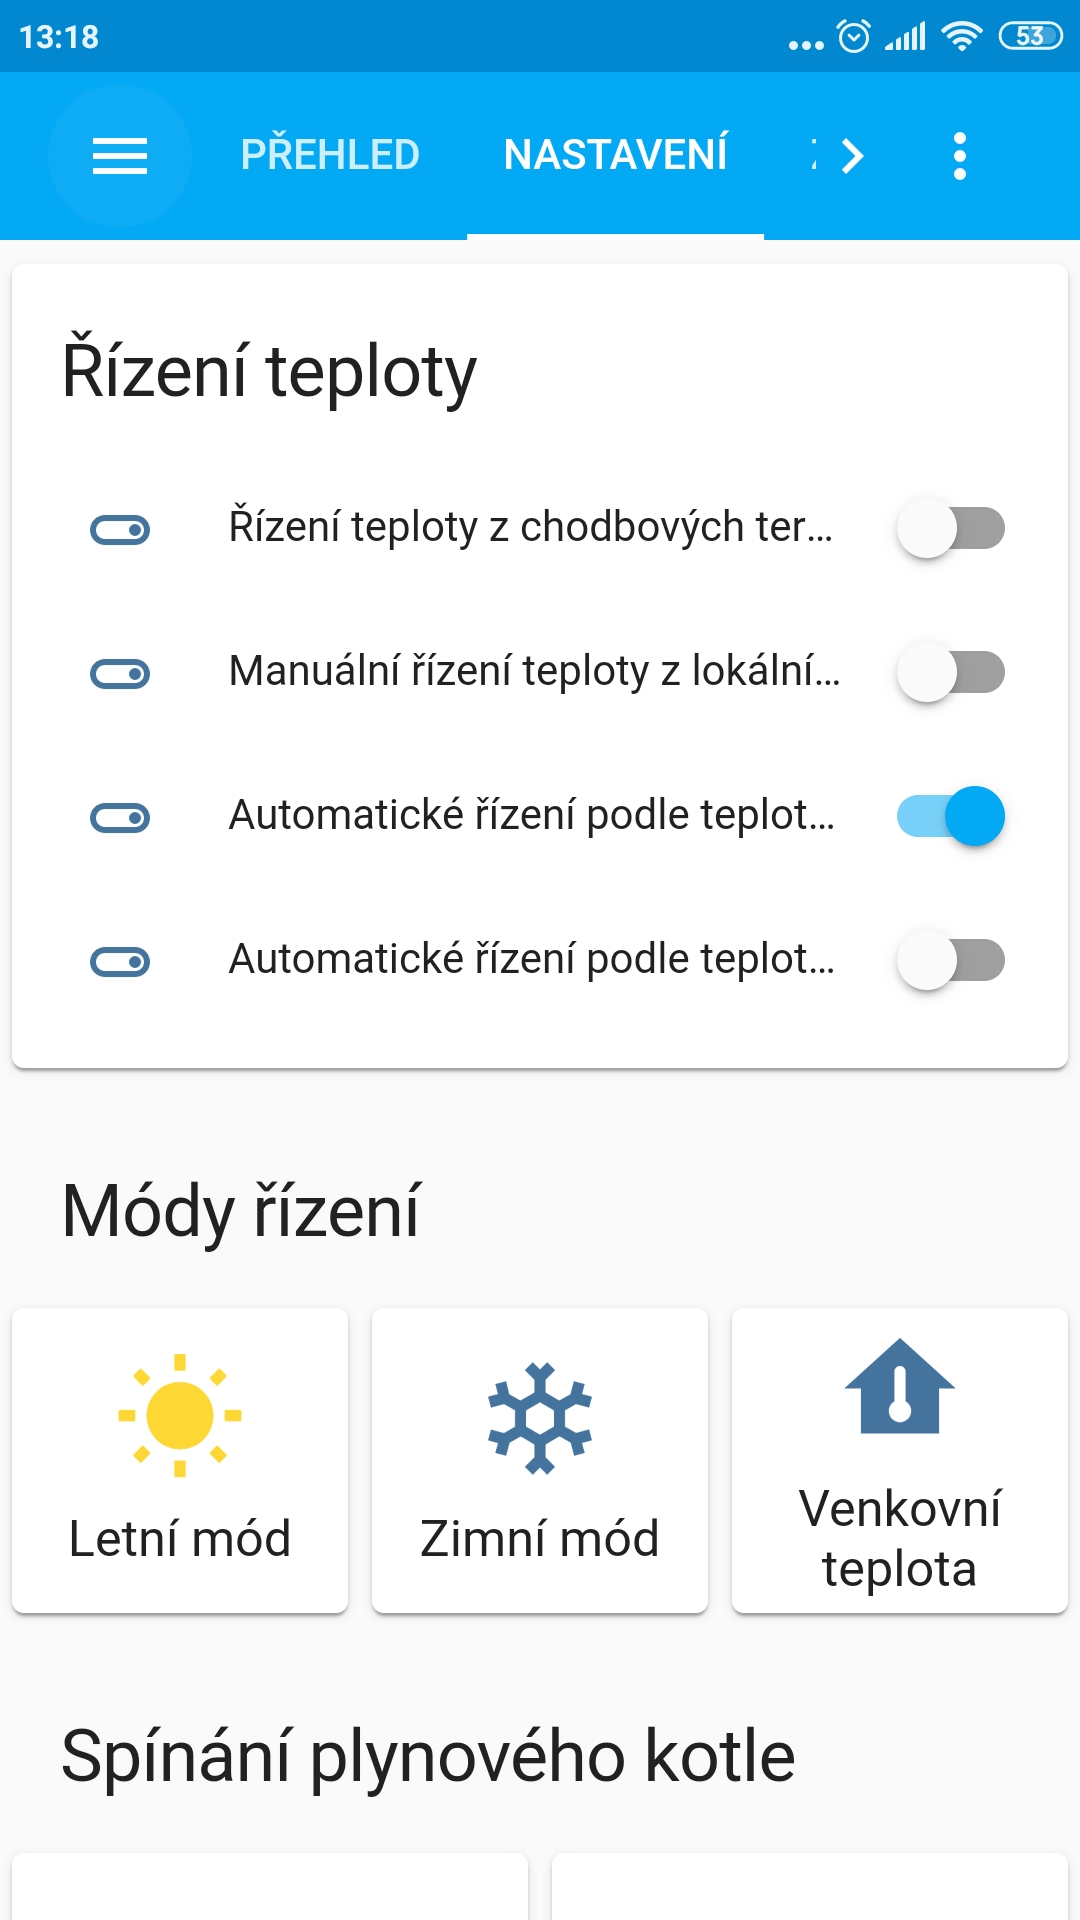
\includegraphics[width=0.8\textwidth]{images/mobilni-aplikace/mobilni-aplikace.png}
%    \caption{Mobilní aplikace na Android.}
%    \label{fig:mobilni-aplikace}
%\end{figure}






\chapter{Testování}

Testování bylo zaměřené jak na hardware, tak software. K testování docházelo postupně s rozvojem celého systému, jak dílčích částí, tak i celku. V následujícím textu jsou popsány jednotlivé softwarové části pro automatizovaný provoz a jejich výsledky při testování.

\subsection{Naměřená data pro řízení podle teplotních plánů}

Bylo provedeno měření teplotních plánů. Cílem bylo zjistit, jak dochází ke zpoždění vytápění na požadovanou teplotu vůči nastavenému časovému plánu. Měření bylo provedeno pro období 19.~11.~2021 od 00:00 do 21 . 11. 2021 do 20:00 pro teplotní plán místnosti „Ložnice rodičů“ (obrázek~\ref{fig:teplotni-plan-loznice-rodicu}). Teplotní úseky pro tento teplotní plán jsou od 00:00–06:30, 06:30–17:00 a 17:00–00:00.

\begin{figure}[H]
    \centering
    \includegraphics[width=0.5\textwidth]{images/testovani/teplotni-plany/teplotni-plan-loznice-rodicu.png}
    \caption{Teplotní plán pro místnost „Ložnice rodičů“}
    \label{fig:teplotni-plan-loznice-rodicu}
\end{figure}

Na následujících grafech je průběh pro aktuální teplotu (modrá křivka), požadovanou teplotu (fialová křivka) a stav topení (oranžová křivka). Na obrázku \ref{fig:loznice-rodicu-termostat-zacatek-vytapeni} je začátek vytápění podle teplotního plánu v intervalu od 17:00–00:00. Podle grafu je aktuální teplot 22 °C, cílová je 23 °C. Této požadované teploty se dosáhne přibližně v čase 19:00 (obrázek \ref{fig:loznice-rodicu-termostat-konec-vytepeni}), zpoždění 2 hodiny vůči začátku časového úseku. Dále podle obrázku \ref{fig:loznice-rodicu-termostat-presazeni-teploty} je vidět setrvačnost podlahového vytápění, která způsobí zvýšení teploty až na 23,5 °C.



\begin{figure}[H]
    \centering
    \includegraphics[width=\textwidth]{images/testovani/teplotni-plany/loznice-rodicu-termostat-zacatek-vytapeni.png}
    \caption{Začátek vytápění v 17:00 pro teplotní úsek 17:00–00:00.}
    \label{fig:loznice-rodicu-termostat-zacatek-vytapeni}
\end{figure}

\begin{figure}[H]
    \centering
    \includegraphics[width=\textwidth]{images/testovani/teplotni-plany/loznice-rodicu-termostat-konec-vytepeni.png}
    \caption{Dosažení požadované teploty přibližně v 19:00.}
    \label{fig:loznice-rodicu-termostat-konec-vytepeni}
\end{figure}

\begin{figure}[H]
    \centering
    \includegraphics[width=\textwidth]{images/testovani/teplotni-plany/loznice-rodicu-termostat-presazeni-teploty.png}
    \caption{Přetopení místnost způsobené setrvačností podlahového vytápění.}
    \label{fig:loznice-rodicu-termostat-presazeni-teploty}
\end{figure}

\subsection{Naměřená data pro řízení podle teplotních plánů s úpravou předpovědi počasí}

\subsection{Detekce otevřeného okna}

\chapter{Návrh dalšího vylepšení}
Vzhledem k používání rekuperace v domě. Rozvést kabely s teplotními senzory do jednotlivých průduchů ve stropě. Snímat výstupní teplotu, která je ochlazena z venkovního prostředí a tuto sníženou teplotu kompenzovat zapnutím vytápění, aby nedocházelo k poklesu teploty v místnosti, respektive její minimalizace.

V budoucnu se počítá s pořízením solárních panelů. Primárním cíle bude ohřívat otopnou vodu v centrálním zásobníku. Přebytky energie ukládat do akumulátorů. Využít stávající systém pro přepínání kam danou energii využít, měřit získanou a spotřebovanou energii.

Doplnit záložní akumulátory v případě výpadku elektrické energie. Zejména pro čerpadla u krbů pro odvedení ohřáté vody z krbového výměníku. V~současné době krby disponují ochranou proti přehřátí spočívající v ochranném ventilu.

V rámci centrálního systému doplnit možnost kopírování teplotních plánů a usnadnit tak jejich tvorbu. 



%\blindmathtrue

%\blinddocument

\chapter{Závěr}
Cílem práce bylo prostudovat problematiku zónového podlahového vytápění a navrhnout vlastní řešení pro řízení dílčích částí systému. Podle zadání diplomové práce se mi povedly splnit všechny body. Navrhl jsem jednotlivé zařízení pro dané části systému, včetně jejich mechanického umístění a ochranných krabiček. Některé části jsem již zakoupil hotové a~případně je upravil. Seznámil jsem se s problematikou POE a navrhl DC/DC měnič pro PSE zařízení. Mezi jednotlivými částmi jsem zvolil vhodnou komunikaci a zejména jednoduchou rozšiřitelnost. Na centrální jednotce funguje open-source řídicí systém pro domácí automatizaci. Tento systém je neustále rozšiřován a aktualizován vývojářskou komunitou. Má již mnoho integrovaných částí pro řízení vytápění. Zároveň existuje již hotová mobilní aplikace, která je se systémem plně funkční, včetně upozorňování uživatelů pro zatopení v krbu. Systém se dá neustále rozšiřovat pro případné požadované úpravy, též software v~nástěnných snímačích prostorové teploty je rychle modifikovatelný. Vše jsem tak mohl upravit podle požadavků uživatelů domu. Zároveň jsem nemusel ztrácet čas nad již hotovým základem softwaru centrální jednotky a více se věnovat samotné automatizaci. Využívám nasbíraná data z jednotlivých místností v~rámci jejich vytápění a na základě nich sestavuji velmi jednoduchou lineární predikci s předpovědí počasí pro úpravu časových teplotních úseků, aby v~požadovaný čas bylo dosaženo požadované teploty. 

Celý systém řízení se postupně vyvíjel. Původně bylo řízení vytápění podle chodbových termostatů a nepočítalo se se zónovým řízením podlahového vytápění. Následně se řízení rozšířilo o zónové vytápění. Majitel domu chtěl primárně veškeré řešení drátové. Proto se nakonec vymýšlelo, jak rozvést kabely do jednotlivých místností. Vznikly primárně POE nástěnné snímače prostorové teploty, využilo se půdy pro rozvedení UTP kabelu do všech místností, kde to bylo možné a zároveň nebyla ničena estetika místnosti. Pro místnosti, kde to nebylo možné, jsem navrhl bezdrátové moduly s napájením ze síťových adaptérů, aby nebylo nutné se starat o výměnu baterií, požadavek majitele. Jako vhodnou formu komunikace jsem zvolil MQTT, kde lze snadno výměnu dat měnit/upravovat/rozšiřovat. Pro kabelové řešení jsem zvolil rovnou napájení po POE, pro bezdrátovou verzi jsem využil již stávající WiFi síť. Zařízení lze tak velmi rychle softwarově modifikovat a~přidávat, to se v~praxi velmi často stávalo. Na verzi s POE jsou poněkud vyšší náklady na součástky, nicméně ty nejdražší součástky mi zaslali výrobci jako vzorek. Jistou nevýhodou mohou být bezdrátové moduly z pohledu bezdrátové komunikace a případných výpadků. Vzhledem k dobrému pokrytí WiFi sítě v~domě je komunikace bezproblémová.

DPS pro vstupy/výstup u centrální jednotky, I$^{2}$C rozdělovač, DPS pro signalizaci u krbů a DPS v rozdělovačích pro podlahové vytápění jsem vyráběl ručně pomocí fotocesty a mokrého leptání. DPS pro nástěnné snímače prostorové teploty jsem nechal vyrobit ve specializované firmě. Následně ručně vyrobené i průmyslově vyrobené DPS jsem vlastnoručně osadil a pájel. Pro plastové krabičky jsem navrhl 3D model a následně vytiskl na 3D tiskárně. Zapojení rozvaděče v technické místnosti i jiných částech jsem též provedl já.

Průběžně jsem při řešení této práce narazil na několik problémů. První z~nich byl správné zvolení impedančního zakončení diferenciální I$^{2}$C sběrnice, které po několikátém předělání nyní funguje bez problémů. Při tisknutí 3D krabičky jsem narazil na problém se správným vytvořením podpěr v oblasti distančních sloupků, aby krabička šla vytisknout. Optimální řešení by bylo krabičku vytisknout bez distančních sloupků, respektive zvlášť a následně je nalepit.



\begin{thebibliography}{3}
% ===== Webove zdroje =====

% === Podlahové vytápění ===
\bibitem{basta-velkoplosne-vytapeni}
BAŠTA, Jiří. Velkoplošné vytápění (I): Úvod do problematiky. \textit{Tzbinfo} [online]. Praha, 26. 6. 2006n. l., \textbf{2006} [cit. 2020-11-01]. Dostupné z: \url{https://vytapeni.tzb-info.cz/3383-velkoplosne-vytapeni-i}
	% ===== Knihy =====
\bibitem{valter-regulace-v-praxi}
VALTER, Jaroslav. \textit{Regulace v praxi: aneb Jak to dělám já}. Praha: BEN --- technická literatura, 2010. ISBN 9788073002565.
	% =================
\bibitem{podlahove-vytapeni-prehled-trhu}
Redakce. Podlahové vytápění - přehled trhu. \textit{TZB-info} [online]. Praha, 2008 [cit. 2020-11-09]. Dostupné z: \url{https://vytapeni.tzb-info.cz/podlahove-vytapeni/4667-podlahove-vytapeni-prehled-trhu}
	% ===== Obrazky =====
\bibitem{vertikalni-prubehy-teplot-pro-ruzne-druhy-vytapeni}
VERMEULEN, Gavin. Heating and Wellbeing [obrázek]. \textit{Heat Pumps} [online]. Austrálie [cit. 2020-11-05]. Dostupné z: \url{http://www.adelaidehydronicheating.com.au/heatpumps.html}
\bibitem{rozlozeni-teplot-podlahove-vytapeni-a-radiatory}
Velkoplošné sálavé systémy --- revoluce ve vytápění a chlazení [obrázek]. \textit{Asb} [online]. Praha, 2016, 29. 9. 2016 [cit. 2020-11-01]. Dostupné z: \url{https://www.asb-portal.cz/stavebnictvi/technicka-zarizeni-budov/vytapeni/velkoplosne-salave-systemy-revoluce-ve-vytapeni-a-chlazeni}
	% ===================
\bibitem{matz-zonove-regulacni-systemy-a-jejich-vyuziti-pri-uspornem-efektivnim-vytapeni}
MATZ, Václav. Zónové regulační systémy a jejich využití při úsporném efektivním vytápění. \textit{TZB-info} [online]. Praha, 2010 [cit. 2020-11-09]. Dostupné z: \url{https://vytapeni.tzb-info.cz/mereni-a-regulace/6203-zonove-regulacni-systemy-a-jejich-vyuziti-pri-uspornem-efektivnim-vytapeni}



% Eletrobock PocketHome
\bibitem{elektrobock-stranky}
Electrobock. \textit{Electrobock} [online]. [cit. 2021-9-1]. Dostupné z: \url{https://www.elektrobock.cz/}
\bibitem{pockethome-stranky}
Pockethome.  \textit{Pockethome} [online]. [cit. 2021-9-1]. Dostupné z: \url{https://pockethome.cz/cs/}
\bibitem{elektrobock-lokalni-termostat}
Bezdrátový vysílač pro podlah.topení PH-BP7-V [obrázek]. \textit{Eletrobock} [online]. Kuřim, 2017 [cit. 2020-11-26]. Dostupné z: \url{https://www.elektrobock.cz/bezdratovy-vysilac-pro-podlah-topeni/p275}
\bibitem{elektrobock-centralni-jednotka}
Produkty --- centrální jednotky [obrázek]. \textit{Pocket home} [online]. Kuřim [cit. 2020-11-26]. Dostupné z: \url{https://pockethome.cz/cs/centralni-jednotky/}
\bibitem{elektrobock-spinaci-jednotka-kotle}
Přijímač kotle-nástěnný PH-PK20 [obrázek]. \textit{Eletrobock} [online]. Kuřim [cit. 2020-11-26]. Dostupné z: \url{https://www.elektrobock.cz/prijimac-kotle-nastenny/p104}
\bibitem{elektrobock-zonovy-regulator}
9-ti kanálový přijímač pro podlah.topení PH-BP1-P9 [obrázek]. \textit{Eletrobock} [online]. Kuřim, 2016 [cit. 2020-11-26]. Dostupné z: \url{https://www.elektrobock.cz/9-ti-kanalovy-prijimac-pro-podlah-topeni/p199}

% Honeywell Evohome
\bibitem{honeywell-evohome-stranky}
Honeywell Evohome. \textit{Honeywell Evohome} [online]. [cit. 2021-9-5]. Dostupné z: \url{https://www.evohome.cz/}
\bibitem{honeywell-lokalni-termostat}
Bezdrátový jednozónový prostorový termostat Honeywell Round T87RF2083 [obrázek]. \textit{Bola: Měřící, regulační a topenářská technika} [online]. Praha [cit. 2020-11-26]. Dostupné z: \url{https://www.bola.cz/bezdratovy-jednozonovy-prostorovy-termostat-honeywell-round-t87rf2025}
\bibitem{honeywell-centralni-jednotka}
Řídící jednotka Evohome Touch Wi-Fi Honeywell ATC928G3026 [obrázek]. \textit{Bola: Měřící, regulační a topenářská technika} [online]. Praha [cit. 2020-11-26]. Dostupné z: \url{https://www.bola.cz/ridici-jednotka-evohome-touch-wi-fi-honeywell-atc928g3026}
\bibitem{honeywell-spinaci-jednotka-kotle}
Bezdrátová reléová jednotka Honeywell Evohome BDR91A1000 [obrázek]. \textit{Bola: Měřící, regulační a topenářská technika} [online]. Praha [cit. 2020-11-26]. Dostupné z: \url{https://www.bola.cz/bezdratova-releova-jednotka-honeywell-evohome-bdr91a1000}
\bibitem{honeywell-rizeni-dobijeni-tuv}
Sada Evohome TV Honeywell ATF500DHW [obrázek]. \textit{Bola: Měřící, regulační a topenářská technika} [online]. Praha [cit. 2020-11-26]. Dostupné z: \url{https://www.bola.cz/sada-evohome-tv-honeywell-atf500dhw}
\bibitem{honeywell-zonovy-regulator}
Honeywell Home podlahový termostat Honeywell evohome HCE80 [obrázek]. \textit{Conrad} [online]. Praha [cit. 2020-11-26]. Dostupné z: \url{https://www.conrad.cz/p/honeywell-home-podlahovy-termostat-honeywell-evohome-hce80-1205666}
\bibitem{honeywell-rozsirujici-modul-pro-zonovy-regulator}
Rozšiřující modul pro HCC80 a HCE80 Honeywell Evohome HCS80 [obrázek]. \textit{Bola: Měřící, regulační a topenářská technika} [online]. Praha [cit. 2020-11-26]. Dostupné z: \url{https://www.bola.cz/rozsirujici-modul-pro-hcc80-a-hce80-honeywell-evohome-hcs80}

% Danfoss Danfoss Link
\bibitem{danfoss-link}
Danfoss Link. \textit{Danfoss} [online]. [cit. 2021-9-5]. Dostupné z: \url{https://www.danfoss.com/cs-cz/campaigns/dhs/smart-heating/danfoss-link/}
\bibitem{danfoss-lokalni-termostat}
Regulační prvky podlahového vytápění, Danfoss Icon 088U1081 [obrázek]. \textit{Danfoss} [online]. [cit. 2020-11-26]. Dostupné z: \url{https://store.danfoss.com/cz/cs/Vyt\%C3\%A1p\%C4\%9Bn\%C3\%AD-a-d\%C3\%A1lkov\%C3\%A9-vyt\%C3\%A1p\%C4\%9Bn\%C3\%AD/Teplovodn\%C3\%AD-podlahov\%C3\%A9-vyt\%C3\%A1p\%C4\%9Bn\%C3\%AD/Prostorov\%C3\%A1-regulace/Regula\%C4\%8Dn\%C3\%AD-prvky-podlahov\%C3\%A9ho-vyt\%C3\%A1p\%C4\%9Bn\%C3\%AD\%2C-Danfoss-Icon/p/088U1081}
\bibitem{danfoss-centralni-jednotka}
Danfoss Link, Central controller, Power supply: PSU 014G0288 [obrázek]. \textit{Danfoss} [online]. [cit. 2020-11-26]. Dostupné z: \url{https://store.danfoss.com/en/Heating-and-District-Energy/Smart-Heating/Danfoss-Link---Smart-Heating/Central-Controller/Danfoss-Link\%E2\%84\%A2\%2C-Central-controller\%2C-Power-supply\%3A-PSU/p/014G0288}
\bibitem{danfoss-zonovy-regulator}
Regulační prvky podlahového vytápění, Danfoss Icon, 230.0 V, Výstup - napětí [V] AC: 230, 8 088U1031 [obrázek]. \textit{Danfoss} [online]. [cit. 2020-11-26]. Dostupné z: \url{https://store.danfoss.com/cz/cs/Vyt\%C3\%A1p\%C4\%9Bn\%C3\%AD-a-d\%C3\%A1lkov\%C3\%A9-vyt\%C3\%A1p\%C4\%9Bn\%C3\%AD/Teplovodn\%C3\%AD-podlahov\%C3\%A9-vyt\%C3\%A1p\%C4\%9Bn\%C3\%AD/Prostorov\%C3\%A1-regulace/Regula\%C4\%8Dn\%C3\%AD-prvky-podlahov\%C3\%A9ho-vyt\%C3\%A1p\%C4\%9Bn\%C3\%AD\%2C-Danfoss-Icon\%2C-230-0-V\%2C-V\%C3\%BDstup---nap\%C4\%9Bt\%C3\%AD-\%5BV\%5D-AC\%3A-230\%2C-8/p/088U1031}
\bibitem{danfoss-spinaci-jednotka-kotle}
Kotlové relé pro systém Danfoss Link, 868.42 MHz 014G0272 [obrázek]. \textit{Danfoss} [online]. [cit. 2020-11-26]. Dostupné z: \url{https://store.danfoss.com/cz/cs/Kotlov\%C3\%A9-rel\%C3\%A9-pro-syst\%C3\%A9m-Danfoss-Link\%2C-868-42-MHz/p/014G0272}

% === MQTT protokol ===
\bibitem{mqtt-specifikace}
MQTT Specifications. \textit{MQTT} [online]. [cit. 2021-11-17]. Dostupné z: \url{https://mqtt.org/mqtt-specification/}
\bibitem{vojacek-mqtt}
VOJÁČEK, Antonín. IoT MQTT prakticky v automatizaci - 1.díl - úvod. \textit{Automatizace.hw.cz: rady a poslední novinky z oboru} [online]. Praha: HW server, 2017 [cit. 2020-12-02]. Dostupné z: \url{https://automatizace.hw.cz/iot-mqtt-prakticky-v-automatizaci-1dil-uvod.html}
\bibitem{maly-mqtt}
MALÝ, Martin. Protokol MQTT: komunikační standard pro IoT. \textit{Root.cz} [online]. Praha, 2016 [cit. 2020-12-02]. Dostupné z: \url{https://www.root.cz/clanky/protokol-mqtt-komunikacni-standard-pro-iot/}

% === I2C sběrnice – teorie ===
\bibitem{i2c-sbernice-specifikace}
UM10204: I2C-bus specification and user manual. \textit{NXP} [online]. Rev. 7.0. 2021 [cit. 2021-11-17]. Dostupné z: \url{https://www.nxp.com/webapp/Download?colCode=UM10204&location=null}. Stažení dokumentu po registraci.
\bibitem{dudka-i2c-relativene-jednoduse}
DUDKA, Michal. I2C --- Relativně jednoduše. \textit{Tajned} [online]. 2016 [cit. 2020-12-03]. Dostupné z: \url{http://www.tajned.cz/2016/10/i2c-relativne-jednoduse/}
\bibitem{olejar-strucny-popis-sbernice-i2c}
OLEJÁR, Martin. Stručný popis sběrnice I2C a její praktické využití k připojení externí eeprom 24LC256 k mikrokontroléru PIC16F877. \textit{Vyvoj.hw.cz: profesionální elektronika} [online]. Praha: HW server, 2000 [cit. 2020-12-03]. Dostupné z: \url{https://vyvoj.hw.cz/navrh-obvodu/strucny-popis-sbernice-i2c-a-jeji-prakticke-vyuziti-k-pripojeni-externi-eeprom-24lc256}
	% === Obrázky === 
\bibitem{i2c-sbernice-datovy-paket-7bit-adresa}
I2C Part 1 - Introducing I2C [obrázek]. \textit{ABelectronics UK} [online]. Swanage, 2020 [cit. 2020-12-03]. Dostupné z: \url{https://www.abelectronics.co.uk/kb/article/1090/i2c-part-1---introducing-i2c}
	% ===============
\bibitem{tisnovsky-komunikace-po-seriove-sbernici-i2c}
TIŠNOVSKÝ, Pavel. Komunikace po sériové sběrnici I2C. \textit{Root} [online]. Praha, 2009 [cit. 2020-12-03]. Dostupné z: \url{https://www.root.cz/clanky/komunikace-po-seriove-sbernici-isup2supc/}



% === 1-Wire sběrnice ===
\bibitem{1-wire-sbernice-specifikace}
READING AND WRITING 1-WIRE® DEVICES THROUGH SERIAL INTERFACES. \textit{Maxim Integraded} [online]. USA: Maxim Integrated, 2009 [cit. 2021-11-17]. Dostupné z: \url{https://www.maximintegrated.com/en/design/technical-documents/app-notes/7/74.html}
\bibitem{maly-1-wire-sbernice}
MALÝ, Martin. Sběrnice 1-Wire. \textit{Vyvoj.hw.cz: profesionální elektronika} [online]. Praha, 2004 [cit. 2020-12-04]. Dostupné z: \url{https://vyvoj.hw.cz/navrh-obvodu/rozhrani/sbernice-1-wiretm.html}
	% === Obrázky === 
\bibitem{1-wire-sbernice-prubehy}
MALÝ, Martin. Sběrnice 1-Wire [obrázek]. \textit{Vyvoj.hw.cz: profesionální elektronika} [online]. Praha, 2004 [cit. 2020-12-04]. Dostupné z: \url{https://vyvoj.hw.cz/navrh-obvodu/rozhrani/sbernice-1-wiretm.html}
	% ===============

% === Home Assistant ==
\bibitem{home-assistant}
Home Assistant. \textit{Home Assistant} [online]. [cit. 2021-11-07]. Dostupné z: \url{https://www.home-assistant.io/}
\bibitem{openhab}
OpenHAB. \textit{OpenHAB} [online]. [cit. 2021-11-07]. Dostupné z: \url{https://www.openhab.org/}
\bibitem{home-assistant-architektura}
Architecture. \textit{Home Assistant Developer Docs} [online]. 2020 [cit. 2020-12-07]. Dostupné z: \url{https://developers.home-assistant.io/docs/architecture\_index}
\bibitem{home-assistant-jadro-architektury}
Core Architecture. \textit{Home Assistant Developer Docs} [online]. [cit. 2021-11-17]. Dostupné z: \url{https://developers.home-assistant.io/docs/architecture/core}
\bibitem{home-assistant-integrace}
Integration Architecture. \textit{Home Assistant Developer Docs} [online]. [cit. 2021-11-17]. Dostupné z: \url{https://developers.home-assistant.io/docs/architecture_components}

% ======================================================================================

% === Centrální jednotka ===
\bibitem{raspberry-pi}
Raspberry Pi. \textit{Raspberry Pi} [online]. [cit. 2021-11-03]. Dostupné z: \url{https://www.raspberrypi.com/products/raspberry-pi-4-model-b/}

% === Teplotní senzory ===
\bibitem{termoclanek-k}
72-21301041-0300-0060.GGP-K GUENTHER. \textit{Tme.cz: Electronic Components} [online]. Polsko [cit. 2020-12-14]. Dostupné z: \url{https://www.tme.eu/cz/details/72-2130104160ggp-k/cidla-teploty-termoclanky/guenther/72-21301041-0300-0060-ggp-k/}
\bibitem{vyrobce-ds18b20}
DS18B20. \textit{Maxim Integraded} [online]. [cit. 2021-11-06]. Dostupné z: \url{https://www.maximintegrated.com/en/products/sensors/DS18B20.html}

% === I2C sběrnice – realizace ===
\bibitem{vyrobce-pca9615}
PCA9615DP: Two-Channel Multipoint Fast-Mode Plus Differential I²C-Bus Buffer with Hot-Swap Logic. \textit{NXP Semiconductors} [online]. [cit. 2021-11-06]. Dostupné z: \url{https://www.nxp.com/products/interfaces/ic-spi-serial-interface-devices/ic-bus-repeaters-hubs-extenders/two-channel-multipoint-fast-mode-plus-differential-ic-bus-buffer-with-hot-swap-logic:PCA9615DP}
\bibitem{pca9615-schema-zapojeni}
PCA9615DP: 2-channel multipoint Fast-mode Plus differential I2C-bus buffer with hot-swap logic. \textit{Nxp.com} [online]. Eindhoven [cit. 2020-12-20]. Dostupné z: \url{https://www.nxp.com/products/interfaces/ic-spi-serial-interface-devices/ic-bus-repeaters-hubs-extenders/2-channel-multipoint-fast-mode-plus-differential-i2c-bus-buffer-with-hot-swap-logic:PCA9615DP}
\bibitem{sm6t6v8cay}
SM6T6V8CAY: Automotive 600 W, 5.8 V TVS in SMB. \textit{STMicroelectronics} [online]. [cit. 2021-11-06]. Dostupné z: \url{https://www.st.com/en/protection-devices/sm6t6v8cay.html}


% === Vstupy/vystupy RPI
\bibitem{ds9503}
DS9503: ESD Protection Diode with Resistors. \textit{Maxim Integraded} [online]. [cit. 2021-11-06]. Dostupné z: \url{https://www.maximintegrated.com/en/products/interface/signal-line-protection-ics/esd-protection-diodes/DS9503.html}
\bibitem{esd9l5-0st5g}
ESD9L: ESD Protection Diode, Ultra Low Capacitance, Unidirectional. \textit{ON Semiconductor} [online]. [cit. 2021-11-06]. Dostupné z: \url{https://www.onsemi.com/products/discrete-power-modules/esd-protection-diodes/esd9l}
\bibitem{bss138p}
BSS138P: 60 V, 360 mA N-channel Trench MOSFET. \textit{Nexperia} [online]. [cit. 2021-11-06]. Dostupné z: \url{https://www.nexperia.com/products/mosfets/automotive-mosfets/BSS138P.html}
\bibitem{max31850k}
MAX31850: Cold-Junction Compensated, 1-Wire Thermocouple-to-Digital Converters. \textit{Maxim Integraded} [online]. [cit. 2021-11-06]. Dostupné z: \url{https://www.maximintegrated.com/en/products/sensors/MAX31850.html}
\bibitem{tps26600}
TPS2660: 4.2-V to 60-V, 150m$\Omega$, 0.1-2.23A eFuse with integrated input reverse polarity protection. \textit{Texas Instruments} [online]. [cit. 2021-11-06]. Dostupné z: \url{https://www.ti.com/product/TPS2660?keyMatch=TPS2660&tisearch=search-everything&usecase=GPN}
\bibitem{rxef005}
RXEF005 - RXEF Series. \textit{Littelfuse} [online]. [cit. 2021-11-06]. Dostupné z: \url{https://www.littelfuse.com/products/polyswitch-resettable-pptcs/radial-leaded/rxef/rxef005.aspx}
\bibitem{sm2t3v3a}
SM2T3V3A: 200 W, 3.3 V TVS in STmite. \textit{STMicroelectronics} [online]. [cit. 2021-11-06]. Dostupné z: \url{https://www.st.com/en/protection-devices/sm2t3v3a.html}

% === Signalizace stavů u krbů
\bibitem{prevodnik-max31850k}
Grove - 1-Wire Thermocouple Amplifier(MAX31850K). \textit{Wiki.seeedstudio.com: The IoT Hardware Enabler} [online]. Čína (Zhongshanyuan Road, Nanshan, Shenzhen) [cit. 2020-12-23]. Dostupné z: \url{https://wiki.seeedstudio.com/Grove-1-Wire\_Thermocouple\_Amplifier-MAX31850K/}
	% ===== Příspěvek na webu =====
\bibitem{hd44780u}
HD44780U (LCD-II). \textit{SparkFun Electronics} [online]. [cit. 2021-11-06]. \url{Dostupné z: https://www.sparkfun.com/datasheets/LCD/HD44780.pdf}. Dokument ve formátu PDF.
	% =============================
\bibitem{pcf8574}
PCF8574: 8-bit 2.5- to 5.5-V I2C/SMBus I/O expander with interrupt. \textit{Texas Instruments} [online]. [cit. 2021-11-06]. Dostupné z: \url{https://www.ti.com/product/PCF8574?keyMatch=PCF8574&tisearch=search-everything&usecase=GPN}
	% === Obrázky ===
\bibitem{lcd-displej}
Modrý LCD displej 16x2, I2C [obrázek]. \textit{Gme.cz} [online]. Praha [cit. 2020-12-23]. Dostupné z: \url{https://www.gme.cz/modry-lcd-display-16x2-i2c}
	% ===============

% === Zónový regulátor ===
\bibitem{pca9685}
PCA9685: 16-Channel, 12-Bit PWM Fm+ I²C-Bus LED Controller. \textit{NXP Semiconductors} [online]. [cit. 2021-11-06]. Dostupné z: \url{https://www.nxp.com/products/power-management/lighting-driver-and-controller-ics/ic-led-controllers/16-channel-12-bit-pwm-fm-plus-ic-bus-led-controller:PCA9685}
\bibitem{dmn3023l}
DMN3023L: N-CHANNEL ENHANCEMENT MODE MOSFE. \textit{Diodes Incorporated} [online]. [cit. 2021-11-06]. Dostupné z: \url{https://www.diodes.com/part/view/DMN3023L}
\bibitem{termoelektricky-pohon-t30nc}
Termoelektrický pohon - NC [obrázek]. \textit{Salus-controls.cz} [online]. [cit. 2020-12-25]. Dostupné z: \url{https://salus-controls.cz/karta-produktu/17/T30NC\_24V\_M30x1\_5}

% === Digitální chodbové termostaty ===
\bibitem{digitalni-termostat-w3230}
Digitální termostat panelový LCD 12V 20A W3230 [obrázek]. \textit{Arduino-shop.cz} [online]. Havlíčkův Brod [cit. 2020-12-25]. Dostupné z: \url{https://arduino-shop.cz/arduino/1980-digitalni-termostat-panelovy-lcd-12v-20a-w3230.html}

% === Spínací jednotka ===
\bibitem{rele-modul-informace}
4 Channel 5V Relay Module. \textit{SunFounder} [online]. [cit. 2021-11-06]. Dostupné z: \url{http://wiki.sunfounder.cc/index.php?title=4_Channel_5V_Relay_Module}
	% === Obrázky ===
\bibitem{ctyr-kanalovy-rele-modul}
JBtek 4-Kanal- DC 5 V Relaismodul für Arduino Raspberry Pi DSP AVR PIC ARM [obrázek]. \textit{Amazon.com} [online]. [cit. 2020-12-25]. Dostupné z: \url{https://www.amazon.com/JBtek-Channel-Module-Arduino-Raspberry/dp/B00KTEN3TM}
	% ===============

% === Rozvaděč ===
\bibitem{mdr-60-5}
MDR-60-5 Mean Well Napájecí spínaný zdroj na DIN li. \textit{Mean Well} [online]. [cit. 2021-11-06]. Dostupné z: \url{https://www.czech-meanwell.cz/meanwell/MDR-60-5-Mean-Well-Napajeci-spinany-zdroj-na-DIN-li-d1491.htm}
\bibitem{hdr-30-12}
HDR-30-12 Mean Well Zdroj na DIN 24W 12V. \textit{Mean Well} [online]. [cit. 2021-11-06]. Dostupné z: \url{https://www.czech-meanwell.cz/meanwell/HDR-30-12-Mean-Well-Zdroj-na-DIN-24W-12V-d5272.htm}
\bibitem{s8vk-c12024}
S8VK-C12024. \textit{Omron} [online]. [cit. 2021-11-06]. Dostupné z: \url{https://industrial.omron.cz/cs/products/S8VK-C12024}

% === Nástěnný snímač prostorové teploty ===
\bibitem{jlcpcb}
JLCPCB. \textit{JLCPCB} [online]. [cit. 2021-11-08]. Dostupné z: \url{https://jlcpcb.com/}
\bibitem{maxlink-psat-10-8p-250}
MaxLink PoE switch PSAT-10-8P-250, 10x LAN/8x PoE 250m, 802.3af/at, 120W, 10/100Mbps. \textit{MaxLink} [online]. [cit. 2021-11-06]. Dostupné z: \url{http://www.maxlink.cz/cs/maxlink-poe-switch-psat-10-8p-250-10x-lan8x-poe-250m-8023afat-120w-10100mbps-87751/product}
	% === Elektronický příspěvek ===
\bibitem{norma-802.3af}
\textit{802.3af-2003 - IEEEE Standard for Information Technology - Telecommunications and Information Exchange Between Systems - Local and Metropolitan Area Networks - Specific Requirements - Part 3: Carrier Sense Multiple Access with Collision Detection (CSMA/CD) Access Method and Physical Layer Specifications - Data Terminal Equipment (DTE) Power Via Media Dependent Interface (MDI)} [online]. IEEE, 2003 [cit. 2021-11-07]. ISBN 978-0-7381-3697-4. Dostupné z: doi:0.1109/IEEESTD.2003.94284
\bibitem{norma-802.3at}
\textit{802.3at-2009 - IEEE Standard for Information technology-- Local and metropolitan area networks-- Specific requirements-- Part 3: CSMA/CD Access Method and Physical Layer Specifications Amendment 3: Data Terminal Equipment (DTE) Power via the Media Dependent Interface (MDI) Enhancements} [online]. IEEE, 2009 [cit. 2021-11-07]. ISBN 978-0-7381-6042-9. Dostupné z: doi:10.1109/IEEESTD.2009.5306743
	% ==============================
\bibitem{tps23753a}
TPS23753A: IEEE 802.3-2005 PoE interface and Isolated Converter controller with Enhanced ESD Ride-Through. \textit{Texas Instruments} [online]. [cit. 2021-11-06]. Dostupné z: \url{https://www.ti.com/product/TPS23753A}
\bibitem{tlv431a}
TLV431A: 1\% accuracy, low-voltage, adjustable precision shunt regulator. \textit{Texas Instruments} [online]. [cit. 2021-11-07]. Dostupné z: \url{https://www.ti.com/product/TLV431A}
\bibitem{esp32-wrover-ie}
ESP32-WROVER-IE(16MB). \textit{ESP Product Selector} [online]. [cit. 2021-11-07]. Dostupné z: \url{https://products.espressif.com/#/product-selector?names=. Výběr modulu ESP32-WROVER-IE(M213EH2864UH3Q0)}.
\bibitem{w5500}
W5500. \textit{Wiznet} [online]. [cit. 2021-11-07]. Dostupné z: \url{https://www.wiznet.io/product-item/w5500/}
\bibitem{lcd-ili9341}
2.2inch SPI Module ILI9341 SKU:MSP2202. \textit{LCDwiki} [online]. [cit. 2021-11-07]. Dostupné z:  \url{http://www.lcdwiki.com/2.2inch_SPI_Module_ILI9341_SKU:MSP2202}
\bibitem{gsm06e05-p1j}
GSM06E05-P1J Mean Well Síťový adaptér Medical 6W 5V. \textit{Mean Well} [online]. [cit. 2021-11-07]. Dostupné z:  \url{https://www.czech-meanwell.cz/meanwell/GSM06E05-P1J-Mean-Well-Sitovy-adapter-Medical-6W-5V-d4278.htm}

% === Krabička pro nástěnný snímač prostorové teploty ===
\bibitem{prusa-i3-mk3s+}
3D TISKÁRNA ORIGINAL PRUSA I3 MK3S+. \textit{Prusa Research by Josef Prusa} [online]. [cit. 2021-11-07]. Dostupné z:  \url{https://www.prusa3d.cz/original-prusa-i3-mk3/}
\bibitem{prusament}
Prusament PETG. \textit{Prusament} [online]. [cit. 2021-11-07]. Dostupné z: \url{https://prusament.com/cs/materials/prusament-petg/}
\bibitem{prusaslicer}
PrusaSlicer. \textit{Prusa Research: by Josef Prusa} [online]. [cit. 2021-11-07]. Dostupné z: \url{https://www.prusa3d.cz/prusaslicer/}
\bibitem{freecad}
FreeCAD. \textit{FreeCAD} [online]. [cit. 2021-11-07]. Dostupné z: \url{https://www.freecadweb.org/}

% === Převodník USB-UART CP2102N ===
\bibitem{cp2102n-miniek}
CP2102N-MINIEK: CP2102N USBXpress Bridge Mini Development Kit. \textit{Silicon Labs} [online]. [cit. 2021-11-07]. Dostupné z: \url{https://www.silabs.com/development-tools/interface/cp2102n-mini-development-kit}

% ======================================================================================

% === Software – Nástěnný snímač prostorové teploty ===
\bibitem{arduino-ide}
Arduino IDE. \textit{Arduino} [online]. [cit. 2021-11-07]. Dostupné z: \url{https://www.arduino.cc/en/software}

\bibitem{teplotni-predikce}
A fancy Home Assistant automation that checks the weather and figures out when to turn on your heater. \textit{Dilettante: Mostly a hobby blog} [online]. [cit. 2021-11-27]. Dostupné z: \url{https://partofthething.com/thoughts/a-fancy-home-assistant-automation-that-checks-the-weather-and-figures-out-when-to-turn-on-your-heater/}


\end{thebibliography}

\appendix

\listofappendices

%\printindex

\chapter{Schéma -- Nástěnný snímač prostorové teploty s Ethernetem}\appcaption{A Schéma -- Nástěnný snímač prostorové teploty s Ethernetem}
\label{app:nastenny-snimac-prostorove-teploty-ethernet}
\includepdf[pages=-,angle=90,pagecommand={\thispagestyle{includedpages}}]{appendix/nastenny-snimac-prostorove-teploty-ethernet/esp32-periferie.pdf}
\includepdf[pages=-,angle=90,pagecommand={\thispagestyle{includedpages}}]{appendix/nastenny-snimac-prostorove-teploty-ethernet/ethernet.pdf}
\includepdf[pages=-,angle=90,pagecommand={\thispagestyle{includedpages}}]{appendix/nastenny-snimac-prostorove-teploty-ethernet/napajeni.pdf}


\chapter{Schéma -- Nástěnný snímač prostorové teploty s WiFi}
\appcaption{B Schéma -- Nástěnný snímač prostorové teploty s WiFi}
\label{app:nastenny-snimac-prostorove-teploty-wifi}
\includepdf[pages=-,angle=90,pagecommand={\thispagestyle{includedpages}}]{appendix/nastenny-snimac-prostorove-teploty-wifi/esp32-periferie.pdf}
\includepdf[pages=-,angle=90,pagecommand={\thispagestyle{includedpages}}]{appendix/nastenny-snimac-prostorove-teploty-wifi/napajeni.pdf}




\chapter{Schéma -- Ostatní}
\appcaption{C Schéma -- Ostatní}
\label{app:schemata-ostatni}
\includepdf[pages=-,angle=90,pagecommand={\thispagestyle{includedpages}}]{appendix/1-wire-koncove-zarizeni/1-wire-1-koncove-zarizeni.pdf}
\includepdf[pages=-,angle=90,pagecommand={\thispagestyle{includedpages}}]{appendix/1-wire-koncove-zarizeni/1-wire-6-koncovych-zarizeni.pdf}

\includepdf[pages=-,angle=90,pagecommand={\thispagestyle{includedpages}}]{appendix/modul-pca9615.pdf}
\includepdf[pages=-,angle=90,pagecommand={\thispagestyle{includedpages}}]{appendix/rozbocovac-i2c.pdf}

\includepdf[pages=-,angle=90,pagecommand={\thispagestyle{includedpages}}]{appendix/vstupy-vystupy-rpi.pdf}

\includepdf[pages=-,angle=90,pagecommand={\thispagestyle{includedpages}}]{appendix/krbova-indikace-1-wire-ochrana-napajeni.pdf}
\includepdf[pages=-,angle=90,pagecommand={\thispagestyle{includedpages}}]{appendix/modul-max31850k.pdf}

\includepdf[pages=-,angle=90,pagecommand={\thispagestyle{includedpages}}]{appendix/zonovy-regulator/ochrany-napajeni-24v-5v.pdf}
\includepdf[pages=-,angle=90,pagecommand={\thispagestyle{includedpages}}]{appendix/zonovy-regulator/svorkovnice-termoelektricke-pohony.pdf}
\includepdf[pages=-,angle=90,pagecommand={\thispagestyle{includedpages}}]{appendix/zonovy-regulator/pca9685.pdf}

\includepdf[pages=-,angle=90,pagecommand={\thispagestyle{includedpages}}]{appendix/rele-modul-jeden-kanal.pdf}

\includepdf[pages=-,angle=90,pagecommand={\thispagestyle{includedpages}}]{appendix/prevodnik-usb-uart.pdf}



\chapter{Krabička pro nástěnný snímač prostorové teploty}
\appcaption{D Krabička pro nástěnný snímač prostorové teploty}
\label{app:krabicka-pro-nastenny-snimac-prostorove-teploty}
\subimport{appendix}{box-wall-sensor-of-room-temperature.tex}

\chapter{Rozdělovač podlahového vytápění}
\appcaption{E Rozdělovač podlahového vytápění}
\label{app:rozdelovac-podlahoveho-vytapeni}
\subimport{appendix}{distributor-first-floor.tex}

\chapter{Ostatní}
\appcaption{F Ostatní}
\label{app:ostatni}
\subimport{appendix}{i2c-module.tex}
\subimport{appendix}{i2c-hub.tex}
\subimport{appendix/software}{block-scheme-wall-sensor-of-room-temperature.tex}

\chapter{Doplňující informace}
\label{doplnujici-informace}
\subimport{appendix}{additional-information.tex}


\chapter{Obsah CD}
\appcaption{G Obsah CD}
\label{app:obsah-cd}
\subimport{appendix}{content-of-cd.tex}

%\bibliographystyle{amsalpha}
%\bibliography{ctutest}
%\printbibliography



\end{document}